\section{Analytická geometrie v prostoru}
\label{sec:Analytic_geometry_space}

V předchozí kapitole jsme se zabývali analytickou geometrií v rovině.
Geometrické útvary jsme popisovali pomocí jejich souřadnic, vektorů
a rovnic a ukázali jsme si, jak lze pomocí algebraických metod zkoumat
jejich vlastnosti a vzájemnou polohu.

Nyní tyto myšlenky rozšíříme do prostoru. Body i vektory již nebudou
mít dvě, ale tři souřadnice, a vedle přímek budeme pracovat také
s rovinami. Řada postupů bude přirozeně navazovat na analytickou
geometrii v rovině, přidání třetího rozměru však přinese také nové
geometrické situace, které v rovině nastat nemohou.

Typickým příkladem jsou dvě přímky. V rovině se dvě přímky s různými
směry vždy protínají. V prostoru však mohou mít různé směry a přesto
nemusí mít žádný společný bod. Takové přímky nazýváme
\textbf{mimoběžné}. Podobně budeme nově zkoumat vztahy mezi přímkami
a rovinami i mezi dvěma rovinami.

Stejně jako v předchozí kapitole budeme vycházet především z již
známých vlastností bodů a vektorů a postupně pomocí nich odvozovat
jednotlivé způsoby analytického popisu geometrických objektů
v prostoru.

\subsection{Přímky v prostoru}
\label{subsec:Lines_in_space}

Stejně jako v rovině je přímka určena jedním svým bodem a směrem,
kterým prochází. Tento směr můžeme vyjádřit pomocí nenulového
směrového vektoru. Známe-li tedy bod
\[
    A[x_A;y_A;z_A]
\]
a nenulový vektor
\[
    \vec{u}=(u_x;u_y;u_z),
\]
je tím určena právě jedna přímka procházející bodem $A$ ve směru
vektoru $\vec{u}$.

Přímku můžeme určit také pomocí dvou různých bodů $A$ a $B$.
Jejím směrovým vektorem potom může být například vektor
\[
    \overrightarrow{AB}=B-A.
\]
Stejně jako v rovině tedy platí, že dvěma různými body prochází právě
jedna přímka.

Analytický popis přímky v prostoru se však od popisu přímky v rovině
v jednom důležitém ohledu liší. V rovině jsme mohli přímku popsat
jedinou obecnou rovnicí
\[
    ax+by+c=0.
\]
V prostoru již jediná lineární rovnice o proměnných $x$, $y$ a $z$
obecně nepopisuje přímku, ale rovinu. Přímku v prostoru proto budeme
nejprve popisovat pomocí \textbf{parametrického vyjádření}, které
přirozeně vychází z bodu přímky a jejího směrového vektoru.

Později si ukážeme, že přímku v prostoru lze popsat také jako
průsečnici dvou rovin.
\subsection{Parametrické vyjádření přímky v prostoru}
\label{subsec:Parametric_line_in_space}

V předchozí části jsme si připomněli, že přímku můžeme určit jedním jejím
bodem a směrem. V prostoru budeme tento směr, stejně jako v rovině,
popisovat pomocí nenulového směrového vektoru.

Uvažujme tedy přímku $p$, která prochází bodem
\[
    A[x_A;y_A;z_A]
\]
a má směrový vektor
\[
    \vec{u}=(u_x;u_y;u_z).
\]

Zvolme nyní libovolný bod $X[x;y;z]$ této přímky. Protože body $A$ a $X$
leží na stejné přímce, je vektor
\[
    \overrightarrow{AX}
\]
rovnoběžný se směrovým vektorem $\vec{u}$. Musí tedy existovat reálné číslo
$t$ takové, že
\[
    \overrightarrow{AX}=t\vec{u}.
\]

Zároveň víme, že
\[
    \overrightarrow{AX}=X-A.
\]
Po dosazení proto dostáváme
\[
    X-A=t\vec{u},
\]
a tedy
\begin{equation}
    X=A+t\vec{u}.
    \label{eq:Parametric_line_in_space_vector}
\end{equation}

Tento vztah má jednoduchý geometrický význam. Začneme v pevném bodě $A$
a přičítáme k němu různé reálné násobky směrového vektoru $\vec{u}$.
Tím získáváme postupně všechny body přímky.

Po rozepsání vztahu~\eqref{eq:Parametric_line_in_space_vector} do
jednotlivých souřadnic dostáváme
\[
    [x;y;z]
    =
    [x_A;y_A;z_A]
    +
    t(u_x;u_y;u_z),
\]
tedy
\[
\begin{aligned}
    p: x&=x_A+t u_x,\\
    y&=y_A+t u_y,\\
    z&=z_A+t u_z; t\in\mathbb{R}.
\end{aligned}
\]

\begin{definition}
    \label{def:Parametric_line_in_space}
    Nechť $A[x_A;y_A;z_A]$ je bod v prostoru a
    $\vec{u}=(u_x;u_y;u_z)$ je nenulový vektor.
    Přímka $p$ procházející bodem $A$ a mající směrový vektor $\vec{u}$
    je množina všech bodů $X[x;y;z]$, které lze vyjádřit ve tvaru
    \[
        X=A+t\vec{u},\qquad t\in\mathbb{R}.
    \]
    V souřadnicích tedy
    \begin{equation}
        \begin{aligned}
            p: x&=x_A+t u_x,\\
            y&=y_A+t u_y,\\
            z&=z_A+t u_z; t\in\mathbb{R}.
        \end{aligned}
        \label{eq:Parametric_line_in_space_coordinates}
    \end{equation}

    Číslo $t$ nazýváme \textbf{parametrem} a vektor $\vec{u}$
    \textbf{směrovým vektorem} přímky.
\end{definition}

Podmínka $\vec{u}\neq\vec{0}$ je nezbytná. Kdyby byl směrový vektor nulový,
potom by pro každé $t\in\mathbb{R}$ platilo
\[
    X=A+t\vec{0}=A.
\]
Místo celé přímky bychom tak získali pouze jediný bod.

Geometrický význam parametru $t$ můžeme vidět na
obrázku~\ref{fig:Parametric_line_in_space}. Pro $t=0$ dostáváme přímo bod
$A$. Pro kladné hodnoty $t$ se z bodu $A$ pohybujeme ve směru vektoru
$\vec{u}$ a pro záporné hodnoty v opačném směru.

\begin{figure}[H]
    \centering
    \begin{tikzpicture}[scale=0.95]

        % Kladné části os
        \draw[->] (0,0,0) -- (5,0,0) node[right] {$x$};
        \draw[->] (0,0,0) -- (0,4.5,0) node[above] {$y$};
        \draw[->] (0,0,0) -- (0,0,4) node[below left] {$z$};

        % Záporné části os
        \draw[->, dashed] (0,0,0) -- (-2,0,0);
        \draw[->, dashed] (0,0,0) -- (0,-2,0);
        \draw[->, dashed] (0,0,0) -- (0,0,-2);

        \node[above left] at (0,0,0) {$O$};

        % Body ležící na přímce
        \coordinate (P1) at (-0.6,-0.2,0);
        \coordinate (Xm) at (0.6,0.7,0.75);
        \coordinate (A)  at (1.8,1.6,1.5);
        \coordinate (Xp) at (3,2.5,2.25);
        \coordinate (P2) at (4.2,3.4,3);
        \coordinate (P0) at (-1.5,-0.87,-0.56);

        % Přímka
        \draw[thick] (P1) -- (P2)
            node[pos=0.96, above] {$p$};
        \draw[thick, dashed] (P0) -- (P1);

        % Směrový vektor
        \draw[vector] (A) -- (Xp)
            node[midway, sloped, above] {$\vec{u}$};

        % Body
        \fill (A) circle (2pt)
            node[below right] {$A=X_0$};

        \fill (Xm) circle (1.7pt)
            node[above left] {$X_{-1}$};

        \fill (Xp) circle (1.7pt)
            node[below right] {$X_1$};

    \end{tikzpicture}
    \caption{Změnou hodnoty parametru $t$ získáváme jednotlivé body
    přímky $p$.}
    \label{fig:Parametric_line_in_space}
\end{figure}

Ze vztahu
\[
    \overrightarrow{AX}=t\vec{u}
\]
navíc vidíme, že absolutní hodnota parametru souvisí se vzdáleností bodu
$X$ od bodu $A$. Platí totiž
\[
    |\overrightarrow{AX}|
    =
    |t\vec{u}|
    =
    |t|\cdot|\vec{u}|.
\]
Například pro $t=2$ se tedy z bodu $A$ posuneme ve směru vektoru
$\vec{u}$ o dvojnásobek jeho velikosti, zatímco pro $t=-2$ o stejnou
vzdálenost v opačném směru.

\begin{example}
    \label{exa:Parametric_line_in_space_point_direction}
    Určete parametrické vyjádření přímky $p$, která prochází bodem
    \[
        A[1;-2;3]
    \]
    a má směrový vektor
    \[
        \vec{u}=(2;1;-1).
    \]

    Použijeme vztah
    \[
        X=A+t\vec{u}.
    \]
    Po dosazení získáme
    \begin{align*}
        X
        &=[1;-2;3]+t(2;1;-1)\\
        &=[1+2t;-2+t;3-t].
    \end{align*}

    Parametrické vyjádření přímky je tedy
    \[
        \begin{aligned}
            p: x&=1+2t,\\
            y&=-2+t,\\
            z&=3-t; t\in\mathbb{R},
        \end{aligned}
    \]
    nebo také ve vektorovém tvaru
    \[
        X=\left\{[1;-2;3]+t(2;1;-1); t\in\mathbb{R}\right\}.
    \]
\end{example}

Z parametrického vyjádření můžeme naopak snadno určit jeden bod přímky
a její směrový vektor. Konstantní členy odpovídají souřadnicím bodu, který
získáme pro $t=0$, zatímco koeficienty u parametru tvoří souřadnice
směrového vektoru.

\begin{example}
    \label{exa:Reading_line_in_space}
    Je dána přímka
    \[
        \begin{aligned}
            q: x&=-3+4t,\\
            y&=2-2t,\\
            z&=1+3t; t\in\mathbb{R}.
        \end{aligned}
    \]
    Určete jeden bod přímky $q$ a její směrový vektor.

    Pro $t=0$ dostáváme
    \[
        x=-3 + 4\cdot 0 = -3,\qquad y=2 - 2\cdot 0 = 2,\qquad z=1 + 3\cdot 0 = 1,
    \]
    a tedy například bod
    \[
        B[-3;2;1].
    \]

    Souřadnice směrového vektoru jsou dány koeficienty u parametru $t$:
    \[
        \vec{v}=(4;-2;3).
    \]

    Přímka $q$ tedy prochází bodem $B[-3;2;1]$ a má směrový vektor
    $\vec{v}=(4;-2;3)$.
\end{example}

Je důležité si uvědomit, že parametrické vyjádření přímky není určeno
jednoznačně. Bod $A$ v zápisu
\[
    X=A+t\vec{u}
\]
může být kterýkoli bod přímky a směrový vektor můžeme nahradit libovolným
jeho nenulovým reálným násobkem.

Je-li tedy $\vec{u}$ směrovým vektorem přímky, potom je jejím směrovým
vektorem také
\[
    k\vec{u},
    \qquad
    k\in\mathbb{R}\setminus\{0\}.
\]

Například přímku
\[
    \begin{aligned}
        p: x&=1+2t,\\
        y&=-2+t,\\
        z&=3-t; t\in\mathbb{R}
    \end{aligned}
\]
můžeme zapsat také pomocí bodu odpovídajícího hodnotě $t=2$:
\[
    B[5;0;1].
\]
Jako nový směrový vektor můžeme zvolit například
\[
    -2\vec{u}=(-4;-2;2).
\]
Dostáváme proto jiné parametrické vyjádření
\[
    \begin{aligned}
        p: x&=5-4s,\\
        y&=-2s,\\
        z&=1+2s; s\in\mathbb{R},
    \end{aligned}
\]
které však popisuje tutéž přímku.

Pomocí parametru můžeme také jednoduše určovat další body přímky. Stačí
za něj dosadit libovolné reálné číslo.

\begin{example}
    \label{exa:Points_on_parametric_line_space}
    Určete body přímky
    \[
        \begin{aligned}
            p: x&=1+2t,\\
            y&=-2+t,\\
            z&=3-t; t\in\mathbb{R}
        \end{aligned}
    \]
    odpovídající hodnotám $t=-1$, $t=0$ a $t=2$.

    Pro $t=-1$ dostáváme
    \[
        X_{-1}
        =
        [1+2(-1);-2+1(-1);3-1(-1)]
        =
        [-1;-3;4].
    \]

    Pro $t=0$ dostáváme
    \[
        X_0 
        = 
        [1+2(0);-2+1(0);3-1(0)] 
        =
        [1;-2;3].
    \]

    Pro $t=2$ dostáváme
    \[
        X_2
        =
        [1+2(2);-2+1(2);3-1(2)]
        =
        [5;0;1].
    \]
\end{example}

Opačnou úlohou je rozhodnout, zda zadaný bod na přímce leží. Bod
$P[x_P;y_P;z_P]$ leží na přímce právě tehdy, když existuje jedna hodnota
parametru $t$, pro kterou současně platí všechny tři parametrické rovnice.

\begin{example}
    \label{exa:Point_membership_line_space}
    Rozhodněte, zda body
    \[
        B[5;0;1]
        \qquad\text{a}\qquad
        C[3;0;2]
    \]
    leží na přímce
    \[
        \begin{aligned}
            p: x&=1+2t,\\
            y&=-2+t,\\
            z&=3-t; t\in\mathbb{R}.
        \end{aligned}
    \]

    Nejprve dosadíme souřadnice bodu $B[5;0;1]$:
    \begin{align*}
        5&=1+2t &&\Rightarrow t=2,\\
        0&=-2+t &&\Rightarrow t=2,\\
        1&=3-t &&\Rightarrow t=2.
    \end{align*}

    Ze všech tří rovnic vyšla stejná hodnota parametru $t=2$, a proto
    bod $B$ na přímce leží:
    \[
        B\in p.
    \]

    Nyní dosadíme souřadnice bodu $C[3;0;2]$:
    \begin{align*}
        3&=1+2t &&\Rightarrow t=1,\\
        0&=-2+t &&\Rightarrow t=2,\\
        2&=3-t &&\Rightarrow t=1.
    \end{align*}

    Neexistuje jediná hodnota parametru, která by současně vyhovovala
    všem třem rovnicím. Proto bod $C$ na přímce neleží:
    \[
        C\notin p.
    \]
\end{example}

Stejnou podmínku můžeme vyjádřit také pomocí vektorů. Je-li přímka určena
bodem $A$ a směrovým vektorem $\vec{u}$, potom bod $P$ leží na této
přímce právě tehdy, když je vektor
\[
    \overrightarrow{AP}
\]
reálným násobkem směrového vektoru $\vec{u}$, tedy když existuje
$t\in\mathbb{R}$ takové, že
\[
    \overrightarrow{AP}=t\vec{u}.
\]

Přímka nemusí být vždy zadána bodem a směrovým vektorem. Velmi často
známe dva různé body
\[
    A[x_A;y_A;z_A],
    \qquad
    B[x_B;y_B;z_B],
\]
kterými má přímka procházet.

Protože dvěma různými body prochází právě jedna přímka, můžeme její
směrový vektor získat přímo jako
\[
    \overrightarrow{AB}
    =
    (x_B-x_A;y_B-y_A;z_B-z_A).
\]

Dosadíme-li tento vektor do vztahu $X=A+t\vec{u}$, dostáváme
\[
    X=A+t\overrightarrow{AB}.
\]
Po rozepsání do souřadnic tedy
\[
    \begin{aligned}
        p: x&=x_A+t(x_B-x_A),\\
        y&=y_A+t(y_B-y_A),\\
        z&=z_A+t(z_B-z_A); t\in\mathbb{R}.
    \end{aligned}
\]

\begin{example}
    \label{exa:Parametric_line_in_space_two_points}
    Určete parametrické vyjádření přímky $r$, která prochází body
    \[
        K[-1;2;4]
        \qquad\text{a}\qquad
        L[3;-2;1].
    \]

    Nejprve určíme směrový vektor přímky:
    \[
        \overrightarrow{KL}
        =
        (3-(-1);-2-2;1-4)
        =
        (4;-4;-3).
    \]

    Použijeme například bod $K[-1;2;4]$ a směrový vektor
    $\overrightarrow{KL}=(4;-4;-3)$. Dostáváme
    \[
        \begin{aligned}
            r: x&=-1+4t,\\
            y&=2-4t,\\
            z&=4-3t; t\in\mathbb{R}.
        \end{aligned}
    \]

    Pro $t=0$ získáme bod $K$ a pro $t=1$ bod
    \[
        [-1+4;2-4;4-3]
        =
        [3;-2;1]
        =
        L.
    \]
    Přímka tedy skutečně prochází oběma zadanými body.
\end{example}

Při určování přímky dvěma body bychom mohli stejně dobře použít bod $L$
a opačný vektor
\[
    \overrightarrow{LK}
    =
    -\overrightarrow{KL}.
\]
Výsledné parametrické vyjádření by vypadalo jinak, ale popisovalo by
stejnou přímku.

\subsection{Vzájemná poloha parametricky vyjádřených přímek v prostoru}
\label{subsec:Relative_position_parametric_lines_space}

V rovině jsme zjistili, že dvě přímky mohou být různoběžné,
rovnoběžné nebo totožné. V prostoru se však objevuje ještě jedna
možnost. Dvě přímky mohou mít různé směry, a přesto se nemusí
protínat. Takové přímky nazýváme \textbf{mimoběžné}.

Uvažujme dvě přímky $p$ a $q$ zadané parametricky ve tvaru
\begin{align}
    p: X &= A+t\vec{u},
    \qquad t\in\mathbb{R},
    \label{eq:Parametric_line_p_relative_position_space}\\
    q: X &= B+s\vec{v},
    \qquad s\in\mathbb{R},
    \label{eq:Parametric_line_q_relative_position_space}
\end{align}
kde $A$ a $B$ jsou zvolené body jednotlivých přímek a
$\vec{u}$ a $\vec{v}$ jsou jejich nenulové směrové vektory.

Stejně jako v rovině používáme pro každou přímku jiný parametr.
Parametr $t$ určuje polohu bodu na přímce $p$, zatímco parametr $s$
určuje polohu bodu na přímce $q$. Pokud se přímky protínají, nemusí
společnému bodu odpovídat stejná hodnota obou parametrů.

Dvě přímky v prostoru mohou být \textbf{různoběžné},
\textbf{rovnoběžné}, \textbf{totožné} nebo \textbf{mimoběžné}.

\begin{definition}
    \label{def:Intersecting_lines_space}
    Dvě přímky v prostoru nazýváme \textbf{různoběžnými}, jestliže
    mají právě jeden společný bod, který nazýváme jejich
    \textbf{průsečíkem}.
\end{definition}

\begin{definition}
    \label{def:Parallel_lines_space}
    Dvě různé přímky v prostoru nazýváme \textbf{rovnoběžnými},
    jestliže mají stejný směr a nemají žádný společný bod.
\end{definition}

\begin{definition}
    \label{def:Coincident_lines_space}
    Dvě přímky v prostoru nazýváme \textbf{totožnými}, jestliže
    mají všechny body společné, a představují tedy tutéž množinu bodů.
\end{definition}

\begin{definition}
    \label{def:Skew_lines_space}
    Dvě přímky v prostoru nazýváme \textbf{mimoběžnými}, jestliže
    nejsou rovnoběžné a nemají žádný společný bod.
\end{definition}

Mimoběžné přímky představují situaci, která v rovině nastat nemůže.
Dvě různoběžné přímky vždy leží v jedné rovině, protože právě dvě
různoběžné přímky rovinu jednoznačně určují. Mimoběžné přímky naopak
v žádné společné rovině neleží.

Jednotlivé možné vzájemné polohy dvou přímek v prostoru jsou
znázorněny na obrázku
\ref{fig:Relative_positions_lines_space}.

\begin{figure}[H]
    \centering

    \tikzset{
        space axes/.style={
            x={(1cm,0cm)},
            y={(0cm,1cm)},
            z={(-0.9cm,-0.5cm)}
        },
        plane/.style={fill=gray!12, draw=gray!50},
        line3d/.style={very thick},
        proj/.style={dashed, gray!70},
        projline/.style={dashed, gray!60},
        point3d/.style={circle, fill=black, inner sep=1.6pt},
        pointproj/.style={circle, fill=gray!65, inner sep=1.5pt}
    }

    \newcommand{\DrawSpaceBase}{%
        \fill[plane] (0,0,0) -- (5,0,0) -- (5,0,3.4) -- (0,0,3.4) -- cycle;
        \node[below right, font=\small] at (3.4,0,3.15) {rovina $xz$ $(y=0)$};

        % kladné části os
        \draw[->] (0,0,0) -- (5.6,0,0) node[right] {$x$};
        \draw[->] (0,0,0) -- (0,4.2,0) node[above] {$y$};
        \draw[->] (0,0,0) -- (0,0,4.1) node[below left] {$z$};

        % záporné části os
        \draw[->, dashed] (0,0,0) -- (-1.1,0,0);
        \draw[->, dashed] (0,0,0) -- (0,-1.0,0);
        \draw[->, dashed] (0,0,0) -- (0,0,-1.0);

        \node[below left] at (0,0,0) {$O$};
    }

    %==================================================
    % RŮZNOBĚŽNÉ
    %==================================================
    \begin{minipage}{0.48\textwidth}
        \centering
        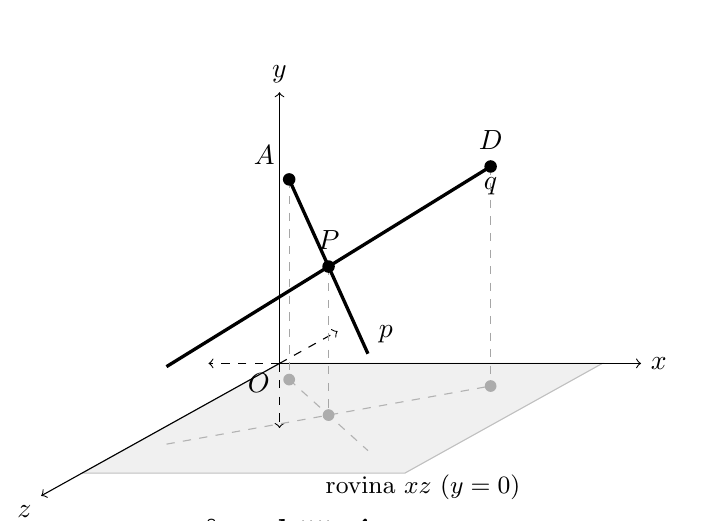
\begin{tikzpicture}[scale=0.82]
            \path[use as bounding box] (-3.9,-2.0) rectangle (6.1,5.2);
            \node[font=\bfseries\large, anchor=west] at (-1.6,-2.6) {různoběžné};

            \begin{scope}[space axes]
                \DrawSpaceBase

                % body
                \coordinate (P) at (2.2,2.3,1.6);
                \coordinate (A) at (0.6,3.1,0.5);
                \coordinate (B) at (3.8,1.5,2.7);

                \coordinate (C) at (0.5,1.2,2.5);
                \coordinate (D) at (3.9,3.4,0.7);

                % průměty
                \coordinate (Pp) at (2.2,0,1.6);
                \coordinate (Ap) at (0.6,0,0.5);
                \coordinate (Bp) at (3.8,0,2.7);
                \coordinate (Cp) at (0.5,0,2.5);
                \coordinate (Dp) at (3.9,0,0.7);

                % průměty přímek do roviny
                \draw[projline] (Ap) -- (Bp);
                \draw[projline] (Cp) -- (Dp);

                % přímky
                \draw[line3d] (A) -- (B) node[above right] {$p$};
                \draw[line3d] (C) -- (D) node[below] {$q$};

                % promítání bodů
                \draw[proj] (A) -- (Ap);
                \draw[proj] (P) -- (Pp);
                \draw[proj] (D) -- (Dp);

                % body v prostoru
                \node[point3d, label=above left:$A$] at (A) {};
                \node[point3d, label=above:$P$] at (P) {};
                \node[point3d, label=above:$D$] at (D) {};

                % body v rovině
                \node[pointproj] at (Ap) {};
                \node[pointproj] at (Pp) {};
                \node[pointproj] at (Dp) {};
            \end{scope}
        \end{tikzpicture}
    \end{minipage}
    \hfill
    %==================================================
    % ROVNOBĚŽNÉ
    %==================================================
    \begin{minipage}{0.48\textwidth}
        \centering
        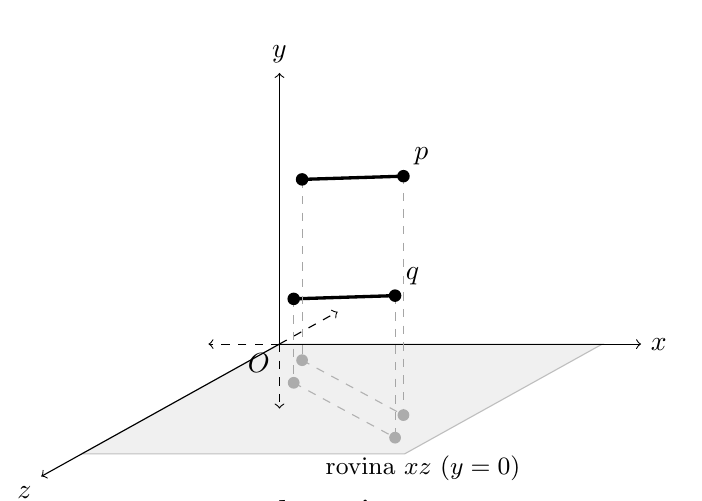
\begin{tikzpicture}[scale=0.82]
            \path[use as bounding box] (-3.9,-2.0) rectangle (6.1,4.9);
            \node[font=\bfseries\large, anchor=west] at (-1.6,-2.6) {rovnoběžné};

            \begin{scope}[space axes]
                \DrawSpaceBase

                % body
                \coordinate (A) at (0.8,2.8,0.5);
                \coordinate (B) at (3.9,3.7,2.2);

                \coordinate (C) at (1.3,1.3,1.2);
                \coordinate (D) at (4.4,2.2,2.9);

                % průměty
                \coordinate (Ap) at (0.8,0,0.5);
                \coordinate (Bp) at (3.9,0,2.2);
                \coordinate (Cp) at (1.3,0,1.2);
                \coordinate (Dp) at (4.4,0,2.9);

                % průměty přímek
                \draw[projline] (Ap) -- (Bp);
                \draw[projline] (Cp) -- (Dp);

                % přímky
                \draw[line3d] (A) -- (B) node[above right] {$p$};
                \draw[line3d] (C) -- (D) node[above right] {$q$};

                % promítání bodů
                \draw[proj] (A) -- (Ap);
                \draw[proj] (B) -- (Bp);
                \draw[proj] (C) -- (Cp);
                \draw[proj] (D) -- (Dp);

                % body v prostoru
                \node[point3d] at (A) {};
                \node[point3d] at (B) {};
                \node[point3d] at (C) {};
                \node[point3d] at (D) {};

                % body v rovině
                \node[pointproj] at (Ap) {};
                \node[pointproj] at (Bp) {};
                \node[pointproj] at (Cp) {};
                \node[pointproj] at (Dp) {};
            \end{scope}
        \end{tikzpicture}
    \end{minipage}

    \vspace{0.8em}

    %==================================================
    % TOTOŽNÉ
    %==================================================
    \begin{minipage}{0.48\textwidth}
        \centering
        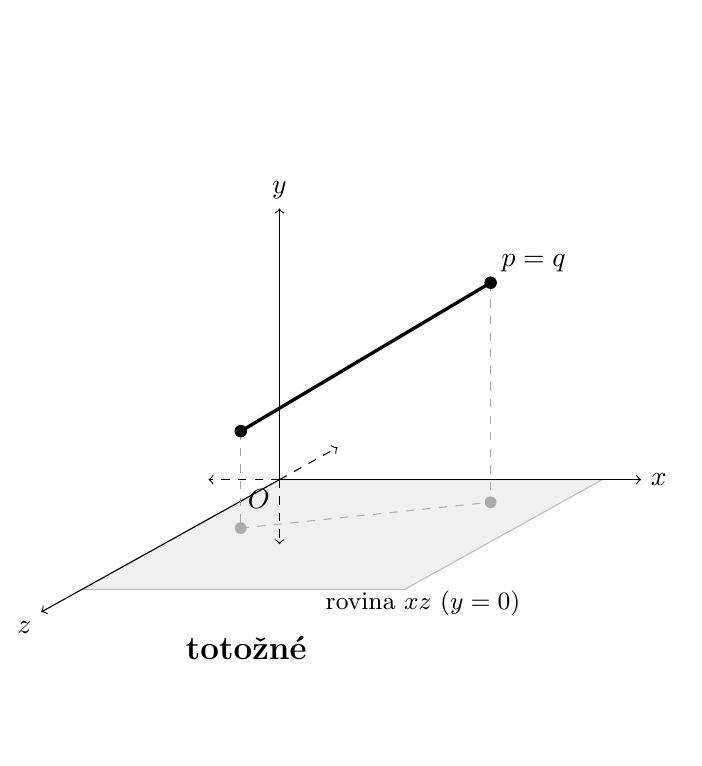
\begin{tikzpicture}[scale=0.82]
            \path[use as bounding box] (-3.9,-4.0) rectangle (6.1,7);
            \node[font=\bfseries\large, anchor=west] at (-1.6,-2.6) {totožné};

            \begin{scope}[space axes]
                \DrawSpaceBase

                % body na jedné přímce
                \coordinate (A) at (0.75,1.5,1.5);
                \coordinate (D) at (3.9,3.4,0.7);

                % průměty
                \coordinate (Ap) at (0.75,0,1.5);
                \coordinate (Dp) at (3.9,0,0.7);

                % průmět přímky
                \draw[projline] (Ap) -- (Dp);

                % přímka
                \draw[line3d] (A) -- (D) node[above right] {$p=q$};

                % promítání bodů
                \draw[proj] (A) -- (Ap);
                \draw[proj] (D) -- (Dp);

                % body v prostoru
                \node[point3d] at (A) {};
                \node[point3d] at (D) {};

                % body v rovině
                \node[pointproj] at (Ap) {};
                \node[pointproj] at (Dp) {};
            \end{scope}
        \end{tikzpicture}
    \end{minipage}
    \hfill
    %==================================================
    % MIMOBĚŽNÉ
    %==================================================
    \begin{minipage}{0.48\textwidth}
        \centering
        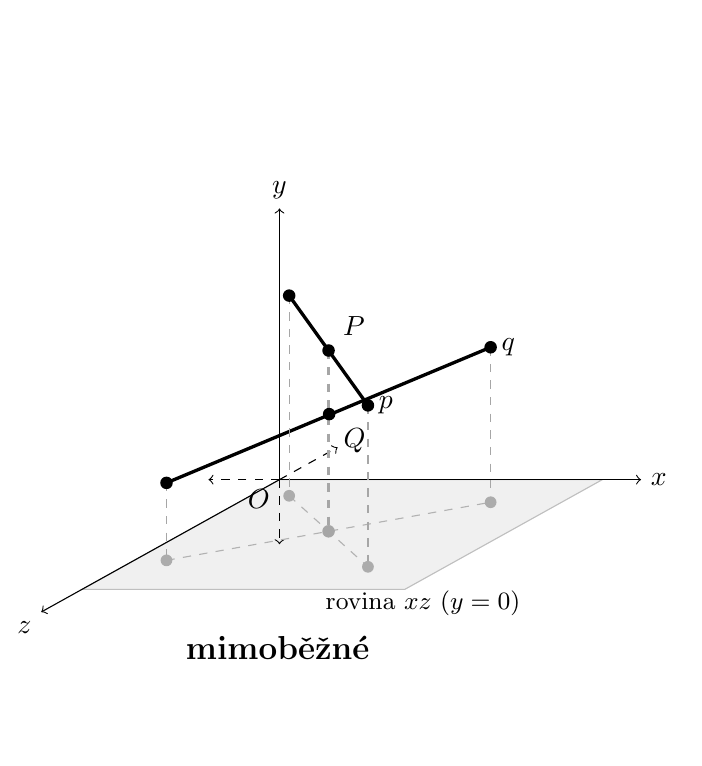
\begin{tikzpicture}[scale=0.82]
            \path[use as bounding box] (-3.9,-4.0) rectangle (6.1,7);
            \node[font=\bfseries\large, anchor=west] at (-1.6,-2.6) {mimoběžné};

            \begin{scope}[space axes]
                \DrawSpaceBase

                % body
                \coordinate (A) at (0.6,3.1,0.5);
                \coordinate (B) at (3.8,2.5,2.7);

                \coordinate (C) at (0.5,1.2,2.5);
                \coordinate (D) at (3.9,2.4,0.7);

                \coordinate (P1) at (2.2,2.8,1.6);
                \coordinate (P2) at (2.2,1.81,1.59);

                % průměty
                \coordinate (Aq) at (0.6,0,0.5);
                \coordinate (Bq) at (3.8,0,2.7);
                \coordinate (Cp) at (0.5,0,2.5);
                \coordinate (Dp) at (3.9,0,0.7);
                \coordinate (Pp) at (2.2,0,1.6);


                % průměty přímek
                \draw[projline] (Aq) -- (Bq);
                \draw[projline] (Cp) -- (Dp);

                % přímky
                \draw[line3d] (A) -- (B) node[right] {$p$};
                \draw[line3d] (C) -- (D) node[right] {$q$};
                \draw[line3d, dashed, gray!70] (P1) -- (Pp);

                % promítání bodů
                \draw[proj] (A) -- (Aq);
                \draw[proj] (B) -- (Bq);
                \draw[proj] (C) -- (Cp);
                \draw[proj] (D) -- (Dp);

                % body v prostoru
                \node[point3d] at (A) {};
                \node[point3d] at (B) {};
                \node[point3d] at (C) {};
                \node[point3d] at (D) {};
                \node[point3d, label=above right:{$P$}] at (P1) {};
                \node[point3d, label=below right:{$Q$}] at (P2) {};
                \node[point3d, gray!70] at (Pp) {};

                % body v rovině
                \node[pointproj] at (Aq) {};
                \node[pointproj] at (Bq) {};
                \node[pointproj] at (Cp) {};
                \node[pointproj] at (Dp) {};
            \end{scope}
        \end{tikzpicture}
    \end{minipage}

    \caption{Možné vzájemné polohy dvou přímek v prostoru.}
    \label{fig:Relative_positions_lines_space}
\end{figure}

Při určování vzájemné polohy budeme stejně jako v rovině nejprve
porovnávat směrové vektory přímek.

Jestliže existuje nenulové číslo $k\in\mathbb{R}$ takové, že
\[
    \vec{v}=k\vec{u},
\]
jsou směrové vektory rovnoběžné a obě přímky mají stejný směr.
V takovém případě mohou být přímky pouze \textbf{rovnoběžné}
nebo \textbf{totožné}. K rozlišení těchto možností stačí ověřit,
zda jeden bod jedné přímky leží také na druhé přímce.

Jestliže směrové vektory $\vec{u}$ a $\vec{v}$ rovnoběžné nejsou,
mají přímky různé směry. V rovině bychom již z této skutečnosti mohli
usoudit, že jsou přímky různoběžné. V prostoru to však neplatí.
Přímky mohou být buď \textbf{různoběžné}, nebo
\textbf{mimoběžné}.

Musíme proto zjistit, zda mají společný bod.

Společný bod musí současně vyhovovat parametrickému vyjádření obou
přímek. Musí tedy existovat hodnoty parametrů $t$ a $s$, pro které
platí
\[
    A+t\vec{u}=B+s\vec{v}.
\]

Jsou-li
\[
    A[x_A;y_A;z_A],
    \qquad
    B[x_B;y_B;z_B],
\]
\[
    \vec{u}=(u_x;u_y;u_z),
    \qquad
    \vec{v}=(v_x;v_y;v_z),
\]
dostáváme soustavu tří rovnic o dvou neznámých parametrech $t$ a $s$:
\begin{equation}
    \begin{cases}
        x_A+t u_x=x_B+s v_x,\\
        y_A+t u_y=y_B+s v_y,\\
        z_A+t u_z=z_B+s v_z.
    \end{cases}
    \label{eq:Intersection_parametric_lines_space}
\end{equation}

Má-li tato soustava řešení, existuje společný bod obou přímek
a přímky jsou různoběžné. Nemá-li soustava řešení, přímky se
neprotínají, a protože jejich směrové vektory nejsou rovnoběžné,
jsou přímky mimoběžné.

Celý rozhodovací postup můžeme shrnout následovně:
\[
\begin{array}{c|c}
\text{Podmínka}
&
\text{Vzájemná poloha přímek}
\\
\hline
\vec{v}=k\vec{u},\ k\neq0,\ B\in p
&
\text{přímky jsou totožné}
\\[1mm]
\vec{v}=k\vec{u},\ k\neq0,\ B\notin p
&
\text{přímky jsou rovnoběžné}
\\[1mm]
\vec{u}\not\parallel\vec{v}
\text{ a soustava \eqref{eq:Intersection_parametric_lines_space} má řešení}
&
\text{přímky jsou různoběžné}
\\[1mm]
\vec{u}\not\parallel\vec{v}
\text{ a soustava \eqref{eq:Intersection_parametric_lines_space} nemá řešení}
&
\text{přímky jsou mimoběžné}
\end{array}
\]

Rozhodovací postup můžeme znázornit také pomocí schématu na obrázku
\ref{fig:Relative_position_parametric_lines_space_decision}.

\begin{figure}[H]
    \centering
    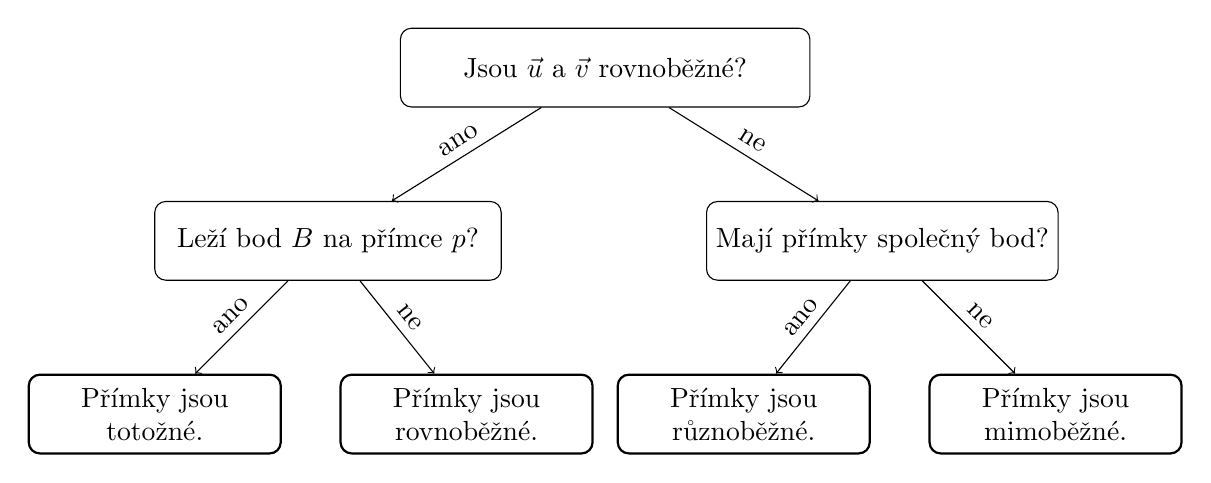
\begin{tikzpicture}[scale=0.88, every node/.style={align=center}]

        % Uzly
        \node[
            draw,
            rounded corners,
            minimum width=5.2cm,
            minimum height=1cm
        ]
        (start) at (0,0)
        {Jsou $\vec{u}$ a $\vec{v}$ rovnoběžné?};

        \node[
            draw,
            rounded corners,
            minimum width=4.4cm,
            minimum height=1cm
        ]
        (point) at (-4,-2.5)
        {Leží bod $B$ na přímce $p$?};

        \node[
            draw,
            rounded corners,
            minimum width=4.4cm,
            minimum height=1cm
        ]
        (intersection) at (4,-2.5)
        {Mají přímky společný bod?};

        \node[
            draw,
            rounded corners,
            minimum width=3.2cm,
            minimum height=1cm,
            thick
        ]
        (coincident) at (-6.5,-5)
        {Přímky jsou\\totožné.};

        \node[
            draw,
            rounded corners,
            minimum width=3.2cm,
            minimum height=1cm,
            thick
        ]
        (parallel) at (-2,-5)
        {Přímky jsou\\rovnoběžné.};

        \node[
            draw,
            rounded corners,
            minimum width=3.2cm,
            minimum height=1cm,
            thick
        ]
        (intersecting) at (2,-5)
        {Přímky jsou\\různoběžné.};

        \node[
            draw,
            rounded corners,
            minimum width=3.2cm,
            minimum height=1cm,
            thick
        ]
        (skew) at (6.5,-5)
        {Přímky jsou\\mimoběžné.};

        % Šipky
        \draw[->] (start) -- (point)
            node[midway, above, sloped] {ano};

        \draw[->] (start) -- (intersection)
            node[midway, above, sloped] {ne};

        \draw[->] (point) -- (coincident)
            node[midway, above, sloped] {ano};

        \draw[->] (point) -- (parallel)
            node[midway, above, sloped] {ne};

        \draw[->] (intersection) -- (intersecting)
            node[midway, above, sloped] {ano};

        \draw[->] (intersection) -- (skew)
            node[midway, above, sloped] {ne};

    \end{tikzpicture}
    \caption{Postup při určování vzájemné polohy parametricky zadaných
    přímek v prostoru.}
    \label{fig:Relative_position_parametric_lines_space_decision}
\end{figure}

\begin{remark}
    Při hledání průsečíku je důležité ověřit \textbf{všechny tři rovnice}
    soustavy~\eqref{eq:Intersection_parametric_lines_space}.
    Vyřešením dvou rovnic můžeme získat konkrétní hodnoty parametrů
    $t$ a $s$, ale tyto hodnoty ještě musí vyhovovat také třetí rovnici.

    Právě v této třetí rovnici se často projeví rozdíl mezi různoběžnými
    a mimoběžnými přímkami.
\end{remark}


\subsubsection{Rovnoběžné přímky}
\label{subsubsec:Parallel_parametric_lines_space}

Jsou-li směrové vektory dvou přímek navzájem rovnoběžné, nemůžeme
pouze z této skutečnosti rozhodnout, zda jsou přímky rovnoběžné,
nebo totožné. Musíme ještě zjistit, zda mají některý bod společný.

\begin{example}
    \label{exa:Parallel_parametric_lines_space}
    Určete vzájemnou polohu přímek $p$ a $q$ zadaných bodem
    a směrovým vektorem:
    \[
        p:\ A[-1;3;2],
        \qquad
        \vec{u}=(-1;2;1),
    \]
    \[
        q:\ B[1;1;0],
        \qquad
        \vec{v}=(2;-4;-2).
    \]

    Nejprve porovnáme směrové vektory. Platí
    \[
        \vec{v}
        =
        (2;-4;-2)
        =
        -2(-1;2;1)
        =
        -2\vec{u}.
    \]

    Směrové vektory jsou tedy rovnoběžné. Přímky $p$ a $q$ jsou
    proto buď rovnoběžné, nebo totožné.

    Ověříme, zda například bod $A[-1;3;2]$ leží na přímce $q$.
    Parametrické vyjádření přímky $q$ je
    \[
        \begin{aligned}
            q: x&=1+2s,\\
            y&=1-4s,\\
            z&=-2s; s\in\mathbb{R}.
        \end{aligned}
    \]

    Dosadíme souřadnice bodu $A$:
    \begin{align*}
        -1&=1+2s
        &&\Rightarrow s=-1,\\
        3&=1-4s
        &&\Rightarrow s=-\frac12,\\
        2&=-2s
        &&\Rightarrow s=-1.
    \end{align*}

    Z jednotlivých rovnic nevychází stejná hodnota parametru.
    Bod $A$ proto na přímce $q$ neleží.

    Přímky mají rovnoběžné směrové vektory, ale nemají žádný
    společný bod. Jsou tedy rovnoběžné:
    \[
        p\parallel q.
    \]
\end{example}

\begin{example}
    \label{exa:Parallel_line_through_origin_space}
    Je dána přímka $p=\left\{\left[2;-1;4\right] + t\left(-3;2;1\right) ; t\in\mathbb{R}\right\}$.
    Určete parametrické vyjádření přímky $q$, která je rovnoběžná
    s přímkou $p$ a prochází počátkem soustavy souřadnic.

    Z parametrického vyjádření přímky $p$ určíme její směrový vektor
    \[
        \vec{u}=(-3;2;1).
    \]

    Má-li být přímka $q$ rovnoběžná s přímkou $p$, můžeme pro ni použít
    stejný směrový vektor, případně libovolný jeho nenulový násobek.

    Přímka $q$ má procházet počátkem soustavy souřadnic
    \[
        O[0;0;0].
    \]

    Použijeme tedy bod $O$ a směrový vektor
    \[
        \vec{u}=(-3;2;1).
    \]

    Parametrické vyjádření hledané přímky je
    \[
        \begin{aligned}
            q: x&=-3s,\\
            y&=2s,\\
            z&=s; s\in\mathbb{R}.
        \end{aligned}
    \]

    Přímky $p$ a $q$ mají stejné směrové vektory, a proto jsou
    rovnoběžné nebo totožné. Protože bod $O[0;0;0]$ na přímce $p$
    neleží, jsou přímky skutečně rovnoběžné:
    \[
        p\parallel q.
    \]
\end{example}

\subsubsection{Různoběžné přímky a jejich průsečík}
\label{subsubsec:Intersecting_parametric_lines_space}

Nejsou-li směrové vektory dvou přímek rovnoběžné, mají přímky
různé směry. Abychom rozhodli, zda jsou různoběžné, nebo mimoběžné,
musíme zjistit, zda mají společný bod.

Průsečík musí současně ležet na obou přímkách. Jeho souřadnice proto
musí vzniknout pro určitou hodnotu parametru $t$ na přímce $p$
a současně pro určitou hodnotu parametru $s$ na přímce $q$.

\begin{remark}
    Stejně jako v rovině musíme při porovnávání dvou parametricky
    vyjádřených přímek používat dva různé parametry:
    \[
        p:\ X=A+t\vec{u},
        \qquad
        q:\ X=B+s\vec{v}.
    \]

    Hodnoty $t$ a $s$ obecně nejsou stejné. Vyjadřují totiž dvě
    různá posunutí ze dvou různých zvolených bodů a pomocí dvou
    různých směrových vektorů.
\end{remark}

\begin{example}
    \label{exa:Intersecting_parametric_lines_space}
    Určete vzájemnou polohu přímek
    \[
        \begin{aligned}
            p: x&=-3+2t,\\
            y&=-1+t,\\
            z&=1; t\in\mathbb{R}
        \end{aligned}
    \]
    a
    \[
        \begin{aligned}
            q: x&=2+s,\\
            y&=-2-3s,\\
            z&=-1-2s; s\in\mathbb{R}.
        \end{aligned}
    \]
    Jsou-li přímky různoběžné, určete jejich průsečík.

    Směrové vektory přímek jsou
    \[
        \vec{u}=(2;1;0),
        \qquad
        \vec{v}=(1;-3;-2).
    \]

    Tyto vektory nejsou rovnoběžné, protože neexistuje číslo
    $k\in\mathbb{R}$, pro které by platilo
    \[
        (1;-3;-2)=k(2;1;0).
    \]

    Přímky jsou tedy buď různoběžné, nebo mimoběžné.
    Pokusíme se najít jejich společný bod.

    Položíme odpovídající souřadnice sobě rovny:
    \begin{align*}
        -3+2t &= 2+s,\\
        -1+t &= -2-3s,\\
        1 &= -1-2s.
    \end{align*}

    Ze třetí rovnice získáme
    \[
        2=-2s
        \qquad\Rightarrow\qquad
        s=-1.
    \]

    Dosadíme tuto hodnotu do první rovnice:
    \begin{align*}
        -3+2t &= 2-1,\\
        -3+2t &= 1,\\
        2t &= 4,\\
        t &= 2.
    \end{align*}

    Nyní musíme ověřit také druhou rovnici:
    \[
        -1+2
        =
        -2-3(-1),
    \]
    tedy
    \[
        1=1.
    \]

    Všechny tři rovnice jsou splněny pro
    \[
        t=2,
        \qquad
        s=-1.
    \]

    Přímky tedy mají společný bod a jsou různoběžné.

    Jeho souřadnice získáme například dosazením $t=2$
    do parametrického vyjádření přímky $p$:
    \begin{align*}
        x&=-3+2\cdot2=1,\\
        y&=-1+2=1,\\
        z&=1.
    \end{align*}

    Průsečíkem přímek je bod
    \[
        P[1;1;1].
    \]

    Zapisujeme
    \[
        p\cap q=\{P[1;1;1]\}.
    \]
\end{example}

\begin{remark}
    Hodnoty parametrů $t$ a $s$ nejsou souřadnicemi průsečíku.
    Určují pouze polohu společného bodu v parametrickém vyjádření
    jednotlivých přímek. Souřadnice průsečíku získáme až jejich
    dosazením do rovnic jedné z přímek.
\end{remark}

\begin{example}
    \label{exa:Perpendicular_lines_through_point_space}
    Je dána přímka
    \[
        \begin{aligned}
            p: x&=-3+2t,\\
            y&=-1+t,\\
            z&=1; t\in\mathbb{R}.
        \end{aligned}
    \]
    a bod $P[1;1;1]$, který na této přímce leží.

    Určete dvě různé přímky $q$ a $r$, které procházejí bodem $P$
    a jsou kolmé k přímce $p$.

    Napřed určíme směrový vektor přímky $p$, který je
    \[
        \vec{u}=(2;1;0).
    \]

    Aby byla přímka $q$ kolmá k přímce $p$, musí její směrový vektor
    $\vec{v}=(v_x;v_y;v_z)$ být kolmý ke směrovému vektoru
    $\vec{u}$. Musí tedy platit
    \[
        \vec{u}\cdot\vec{v}=0.
    \]

    Po dosazení získáme
    \[
        (2;1;0)\cdot(v_x;v_y;v_z)=0,
    \]
    tedy
    \[
        2v_x+v_y=0.
    \]

    Tato rovnice neurčuje směrový vektor jednoznačně. Protože dostáváme jednu rovnici o dvou neznámých,
    máme nekonečně mnoho řešení. Můžeme tedy jednu souřadnici libovolně zvolit, například
    zvolit $v_x=1$ a využít toho, že $v_z=0$ a dosadit potom do rovnice
    \[
        2\cdot1+v_y=0,
    \]
    a tedy
    \[
        v_y=-2.
    \]

    Jedním vhodným směrovým vektorem je proto
    \[
        \vec{v}=(1;-2;0).
    \]

    Přímka $q$ procházející bodem $P[1;1;1]$ má parametrické
    vyjádření
    \[
        \begin{aligned}
            q: x&=1+s,\\
            y&=1-2s,\\
            z&=1; s\in\mathbb{R}.
        \end{aligned}
    \]

    Můžeme však zvolit také například
    \[
        v_x=0,\qquad v_y=0,\qquad v_z=1,
    \]
    protože
    \[
        (2;1;0)\cdot(0;0;1)=0.
    \]

    Dostáváme tedy druhý směrový vektor
    \[
        \vec{w}=(0;0;1)
    \]
    a druhou kolmou přímku
    \[
        \begin{aligned}
            r: x&=1,\\
            y&=1,\\
            z&=1+\lambda; \lambda\in\mathbb{R}.
        \end{aligned}
    \]

    Obě přímky $q$ a $r$ procházejí bodem $P$, ve kterém protínají
    přímku $p$, a jejich směrové vektory jsou kolmé ke směrovému
    vektoru přímky $p$. Platí tedy
    \[
        q\perp p
        \qquad\text{a}\qquad
        r\perp p.
    \]
\end{example}

\begin{remark}
    V rovině prochází daným bodem přímky právě jedna přímka, která je
    k této přímce kolmá. V prostoru je situace jiná.

    Pro směrový vektor
    \[
        \vec{u}=(2;1;0)
    \]
    musí směrový vektor každé kolmé přímky splňovat pouze podmínku
    \[
        2v_x+v_y=0.
    \]
    Souřadnici $v_z$ můžeme volit libovolně a stejně tak můžeme volit
    jednu ze souřadnic $v_x$ a $v_y$ a druhou dopočítat. Existuje proto
    nekonečně mnoho různých směrů kolmých k vektoru $\vec{u}$.

    Bodem $P$ tak v prostoru prochází nekonečně mnoho přímek kolmých
    k přímce $p$. Všechny tyto přímky společně vyplňují jednu rovinu,
    která prochází bodem $P$ a je kolmá k přímce $p$.

    S touto rovinou a jejím analytickým popisem se seznámíme později.
\end{remark}

\subsubsection{Mimoběžné přímky}
\label{subsubsec:Skew_parametric_lines_space}

Mimoběžné přímky mají různé směry, ale nemají žádný společný bod.
Při jejich určování proto nejprve zjistíme, že jejich směrové vektory
nejsou rovnoběžné, a poté ověříme, že soustava rovnic pro společný bod
nemá řešení.

\begin{example}
    \label{exa:Skew_parametric_lines_space}
    Určete vzájemnou polohu přímek $p=\left\{\left[2;3;-1\right] + t\left(1;-2;1\right); t\in\mathbb{R}\right\}$
    a
    \[
        \begin{aligned}
            q: x&=-2+3s,\\
            y&=3+2s,\\
            z&=3+s; s\in\mathbb{R}.
        \end{aligned}
    \]

    Směrové vektory přímek jsou
    \[
        \vec{u_p}=(1;-2;1),
        \qquad
        \vec{v_q}=(3;2;1).
    \]

    Směrové vektory nejsou rovnoběžné, protože neexistuje číslo
    $k\in\mathbb{R}$ takové, že
    \[
        \vec{v_q}=k\vec{u_p}.
    \]

    Přímky mohou být různoběžné nebo mimoběžné. Zjistíme tedy,
    zda mají společný bod.

    Položíme odpovídající souřadnice sobě rovny:
    \begin{align*}
        2+t &= -2+3s,\\
        3-2t &= 3+2s,\\
        -1+t &= 3+s.
    \end{align*}

    Ze třetí rovnice vyjádříme parametr $t$:
    \[
        t=s+4.
    \]

    Dosadíme jej do první rovnice:
    \begin{align*}
        2+(s+4) &= -2+3s,\\
        6+s &= -2+3s,\\
        8 &= 2s,\\
        s &= 4.
    \end{align*}

    Nyní však musíme zkontrolovat také druhou rovnici.
    Dosadíme do ní $t=s+4$:
    \begin{align*}
        3-2(s+4) &= 3+2s,\\
        3-2s-8 &= 3+2s,\\
        -5-2s &= 3+2s,\\
        -8 &= 4s,\\
        s &= -2.
    \end{align*}

    Z první a druhé rovnice jsme po použití třetí rovnice získali
    dvě různé hodnoty parametru:
    \[
        s=4
        \qquad\text{a}\qquad
        s=-2.
    \]

    Neexistuje tedy dvojice parametrů $t$ a $s$, která by současně
    splňovala všechny tři rovnice. Přímky nemají společný bod.

    Protože zároveň nemají rovnoběžné směrové vektory, jsou
    \textbf{mimoběžné}.
\end{example}

\begin{remark}
    Právě u mimoběžných přímek je obzvlášť důležité nepřestat
    s výpočtem po vyřešení pouze dvou rovnic. Dvě rovnice o dvou
    neznámých mohou mít řešení, ale třetí rovnice může ukázat,
    že nalezená dvojice parametrů společnému bodu obou přímek
    neodpovídá.
\end{remark}

\begin{example}
    \label{exa:Construct_skew_line_space}

    Je dána přímka $p=\left\{\left[2;3;-1\right] + t\left(1;-2;1\right); t\in\mathbb{R}\right\}$.
    Určete parametrické vyjádření přímky $q$, která prochází bodem $B[0;1;2]$ a je rovnoběžná s osou $z$. 
    Poté určete vzájemnou polohu přímek $p$ a $q$.

    Přímka rovnoběžná s osou $z$ má směrový vektor například
    \[
        \vec{v}=(0;0;1).
    \]

    Protože má přímka $q$ procházet bodem $B[0;1;2]$, dostáváme tedy přímku $q=B+s\cdot \vec{v}$ můžeme ji
    zapsat parametricky ve tvaru
    \[
        \begin{aligned}
            q: x&=0,\\
            y&=1,\\
            z&=2+s; s\in\mathbb{R}.
        \end{aligned}
    \]

    Směrový vektor přímky $p$ je
    \[
        \vec{u}=(1;-2;1).
    \]

    Vektory
    \[
        \vec{u}=(1;-2;1)
        \qquad\text{a}\qquad
        \vec{v}=(0;0;1)
    \]
    nejsou rovnoběžné. Přímky $p$ a $q$ tedy mohou být různoběžné
    nebo mimoběžné.

    Zjistíme, zda mají společný bod. Položíme odpovídající souřadnice
    sobě rovny:
    \[
        \begin{cases}
            2+t=0,\\
            3-2t=1,\\
            -1+t=2+s.
        \end{cases}
    \]

    Z první rovnice dostáváme
    \[
        t=-2.
    \]

    Po dosazení do druhé rovnice však získáme
    \[
        3-2(-2)=1,
    \]
    tedy
    \[
        7=1,
    \]
    což není pravda.

    Přímky proto nemají společný bod. Protože současně nejsou
    rovnoběžné, jsou \textbf{mimoběžné}.
\end{example}

\begin{example}
    \label{exa:Line_intersecting_q_parallel_p}

    Jsou dány mimoběžné přímky
    \[
        \begin{aligned}
            p: x&=2+t,\\
            y&=3-2t,\\
            z&=-1+t; t\in\mathbb{R}
        \end{aligned}
    \]
    a
    \[
        \begin{aligned}
            q: x&=-2+3s,\\
            y&=3+2s,\\
            z&=3+s; s\in\mathbb{R}.
        \end{aligned}
    \]

    Najděte přímku $r$, která je rovnoběžná s přímkou $p$
    a zároveň je různoběžná s přímkou $q$.

    Směrový vektor přímky $p$ je
    \[
        \vec{u}=(1;-2;1).
    \]

    Má-li být přímka $r$ rovnoběžná s přímkou $p$, můžeme jako její
    směrový vektor použít právě vektor
    \[
        \vec{u}=(1;-2;1).
    \]

    Zároveň chceme, aby přímka $r$ protínala přímku $q$.
    Zvolíme proto libovolný bod na přímce $q$.
    Nejjednodušší je položit
    \[
        s=0.
    \]

    Dostáváme bod
    \[
        B[-2;3;3].
    \]

    Přímka $r$ procházející bodem $B$ a mající směrový vektor
    $\vec{u}=(1;-2;1)$ má tedy parametrické vyjádření
    \[
        \begin{aligned}
            r: x&=-2+\lambda,\\
            y&=3-2\lambda,\\
            z&=3+\lambda; \lambda\in\mathbb{R}.
        \end{aligned}
    \]

    Přímky $p$ a $r$ mají stejné směrové vektory, proto
    \[
        r\parallel p.
    \]

    Přímka $r$ zároveň prochází bodem $B[-2;3;3]$, který leží také
    na přímce $q$. Platí tedy
    \[
        r\cap q=\{B\}.
    \]

    Směrový vektor přímky $q$ je
    \[
        \vec{v}=(3;2;1),
    \]
    který není rovnoběžný s vektorem
    \[
        \vec{u}=(1;-2;1).
    \]

    Přímky $q$ a $r$ tedy mají právě jeden společný bod, a jsou proto
    \textbf{různoběžné}.

    Hledaná přímka může být například
    \[
        \begin{aligned}
            r: x&=-2+\lambda,\\
            y&=3-2\lambda,\\
            z&=3+\lambda; \lambda\in\mathbb{R}.
        \end{aligned}
    \]
\end{example}

\begin{remark}
    Hledaná přímka $r$ není určena jednoznačně.

    V předchozím příkladu jsme zvolili bod přímky $q$ odpovídající
    hodnotě $s=0$. Mohli bychom však zvolit libovolnou jinou hodnotu
    parametru $s$.

    Obecný bod přímky $q$ má souřadnice
    \[
        Q_s[-2+3s;3+2s;3+s].
    \]

    Každým takovým bodem můžeme vést přímku se směrovým vektorem
    přímky $p$,
    \[
        \vec{u}=(1;-2;1).
    \]

    Dostáváme tak celou soustavu přímek
    \[
        \begin{aligned}
            r_s: x&=-2+3s+\lambda,\\
            y&=3+2s-2\lambda,\\
            z&=3+s+\lambda;
            \qquad s,\lambda\in\mathbb{R}.
        \end{aligned}
    \]

    Pro každou pevně zvolenou hodnotu $s$ dostaneme jednu přímku
    $r_s$, která protíná přímku $q$ a je rovnoběžná s přímkou $p$.

    Takových přímek tedy existuje nekonečně mnoho.

    Zajímavé je, že všechny tyto přímky společně vyplňují jednu
    rovinu. Ta obsahuje přímku $q$ a je rovnoběžná s přímkou $p$.
    S takovým popisem roviny se seznámíme opět v následujících kapitolách.
\end{remark}


\subsubsection{Totožné přímky}
\label{subsubsec:Coincident_parametric_lines_space}

Jsou-li směrové vektory dvou přímek rovnoběžné a zároveň jeden bod
první přímky leží na druhé přímce, mají přímky stejný směr i společný
bod. V takovém případě představují tutéž množinu bodů a jsou totožné.

\begin{example}
    \label{exa:Coincident_parametric_lines_space}
    Určete vzájemnou polohu přímek
    \[
        \begin{aligned}
            p: x&=-3+4t,\\
            y&=4-2t,\\
            z&=2+2t; t\in\mathbb{R}
        \end{aligned}
    \]
    a
    \[
        \begin{aligned}
            q: x&=1-6s,\\
            y&=2+3s,\\
            z&=4-3s; s\in\mathbb{R}.
        \end{aligned}
    \]

    Z parametrických rovnic vyčteme směrové vektory
    \[
        \vec{u}=(4;-2;2),
        \qquad
        \vec{v}=(-6;3;-3).
    \]

    Platí
    \[
        \vec{v}
        =
        -\frac32\vec{u},
    \]
    takže směrové vektory jsou rovnoběžné.

    Přímky jsou tedy buď rovnoběžné, nebo totožné.

    Přímka $q$ prochází například bodem
    \[
        B[1;2;4],
    \]
    který získáme pro $s=0$.

    Ověříme, zda tento bod leží také na přímce $p$:
    \begin{align*}
        1&=-3+4t
        &&\Rightarrow t=1,\\
        2&=4-2t
        &&\Rightarrow t=1,\\
        4&=2+2t
        &&\Rightarrow t=1.
    \end{align*}

    Ze všech tří rovnic vyšla stejná hodnota parametru $t=1$.
    Bod $B$ tedy leží na přímce $p$.

    Přímky mají rovnoběžné směrové vektory a společný bod,
    a proto jsou totožné:
    \[
        p=q.
    \]

    Jejich průnikem je celá přímka:
    \[
        p\cap q=p=q.
    \]
\end{example}

Vzájemnou polohu dvou parametricky vyjádřených přímek v prostoru
tedy určujeme ve dvou krocích. Nejprve porovnáme jejich směrové
vektory. Jsou-li rovnoběžné, rozhodujeme mezi rovnoběžnými a
totožnými přímkami pomocí společného bodu. Nejsou-li rovnoběžné,
hledáme průsečík. Podle toho, zda společný bod existuje, jsou
přímky různoběžné, nebo mimoběžné.

\begin{example}
    \label{exa:Parametric_z_axis}
    Určete parametrické vyjádření osy $z$.

    Osa $z$ prochází počátkem soustavy souřadnic
    \[
        O[0;0;0]
    \]
    a její směr je určen například vektorem
    \[
        \vec{u}=(0;0;1).
    \]

    Použijeme vztah
    \[
        X=O+t\vec{u}.
    \]
    Dostáváme
    \[
        [x;y;z]
        =
        [0;0;0]+t(0;0;1),
    \]
    a tedy
    \[
        \begin{aligned}
            z: x&=0,\\
            y&=0,\\
            z&=t; t\in\mathbb{R}.
        \end{aligned}
    \]

    Osa $z$ je tedy tvořena právě body, jejichž první dvě souřadnice
    jsou nulové a třetí souřadnice může nabývat libovolné reálné hodnoty.
\end{example}

\begin{example}
    \label{exa:Relative_position_lines_cube}
    Je dána krychle $ABCDEFGH$ o hraně délky $4$, přičemž $A[0;0;4], B[4;0;4],$ 
    
    $H[0;4;0]$.
    Body $K,L,M,N,P,Q$ jsou po řadě středy hran
    $AB$, $BF$, $BC$, $GH$, $AE$, $EH$.
    a bod $R$ leží na hraně $AB$ tak, že $|AR|=1$.

    \begin{figure}[H]
        \centering
        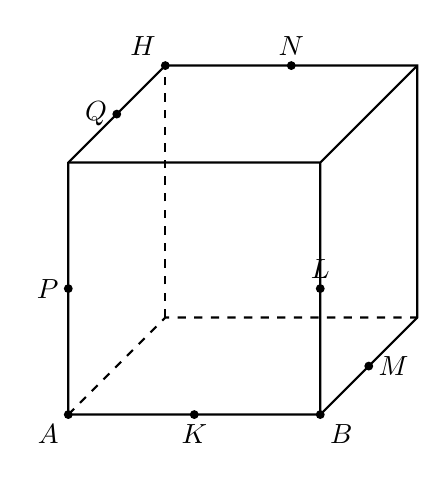
\begin{tikzpicture}[scale=0.8]
            % Vrcholy krychle
            \coordinate (A) at (0,0,4);
            \coordinate (B) at (4,0,4);
            \coordinate (C) at (4,0,0);
            \coordinate (D) at (0,0,0);
            \coordinate (E) at (0,4,4);
            \coordinate (F) at (4,4,4);
            \coordinate (G) at (4,4,0);
            \coordinate (H) at (0,4,0);

            % Středové body hran
            \coordinate (K) at (2,0,4);
            \coordinate (L) at (4,2,4);
            \coordinate (M) at (4,0,2);
            \coordinate (N) at (2,4,0);
            \coordinate (P) at (0,2,4);
            \coordinate (Q) at (0,4,2);

            % Hrany krychle
            \draw[thick] (A) -- (B) -- (C) -- (G) -- (H) -- (E) -- (A);
            \draw[thick] (E) -- (F) -- (B) -- (F) -- (G);
            \draw[dashed, thick] (A) -- (D) -- (C);
            \draw[dashed, thick] (D) -- (H);

            % Body A, B, H
            \fill (A) circle (2pt) node[below left] {$A$};
            \fill (B) circle (2pt) node[below right] {$B$};
            \fill (H) circle (2pt) node[above left] {$H$};

            % Body K, L, M, N, P, Q, R
            \fill (K) circle (2pt) node[below] {$K$};
            \fill (L) circle (2pt) node[above] {$L$};
            \fill (M) circle (2pt) node[right] {$M$};
            \fill (N) circle (2pt) node[above] {$N$};
            \fill (P) circle (2pt) node[left] {$P$};
            \fill (Q) circle (2pt) node[left] {$Q$};

        \end{tikzpicture}
        \caption{Krychle a vyznačené body k příkladu.}
    \end{figure}

    Určete vzájemnou polohu přímek
    \begin{enumerate}[label=\alph*)]
        \item $KL$ a $MN$,
        \item $AK$ a $EM$,
        \item $KQ$ a $CN$,
        \item $KP$ a $CH$,
        \item $AQ$ a $CN$.
    \end{enumerate}

    Nejprve určíme souřadnice bodů, které budeme v jednotlivých částech
    potřebovat. Z daných souřadnic vrcholů krychle dostáváme
    \[
        D[0;0;0],\qquad E[0;4;4],\qquad
        C[4;0;4],\qquad F[4;4;4],\qquad G[4;4;0].
    \]
    Protože body $K,L,M,N,P,Q$ jsou středy příslušných hran, platí
    \[
        K[2;0;4],\qquad L[4;2;4],\qquad M[4;0;2],
    \]
    \[
        N[2;4;0],\qquad P[0;2;4],\qquad Q[0;4;2].
    \]

    \textbf{a) Určeme vzájemnou polohu přímek $KL$ a $MN$.}

    Směrový vektor přímky $KL$ je
    \[
        \overrightarrow{KL}
        =L-K
        =(4-2;2-0;4-4)
        =(2;2;0).
    \]

    Směrový vektor přímky $MN$ je
    \[
        \overrightarrow{MN}
        =N-M
        =(2-4;4-0;0-4)
        =(-2;4;-4).
    \]

    Směrové vektory nejsou násobky, tudíž přímky nejsou rovnoběžné.
    Mohou být různoběžné, nebo mimoběžné. Zjistíme tedy, zda mají společný bod.

    \begin{align*}
        p_{KL}: x&=2+2t,\\
                y&=0+2t,\\
                z&=4+0t; t\in\mathbb{R},\\
        p_{MN}: x&=4-2s,\\
                y&=0+4s,\\
                z&=2-4s; s\in\mathbb{R}.
    \end{align*}

    Pro společný bod musí platit, že existují hodnoty parametrů $t$ a $s$, pro které současně platí
    \begin{align*}
        2+2t&=4-2s,\\
        0+2t&=0+4s,\\
        4+0t&=2-4s.
    \end{align*}

    Z druhé rovnice dostáváme:
    \[
    t=2s,
    \]
    Po dosazení do první rovnice dostáváme:
    \begin{align*}
        2+2(2s)&=4-2s,\\
        2+4s&=4-2s,\\
        6s&=2,\\
        s&=\frac13,
    \end{align*}

    Poté hodnota parametru $t$ je $t=\frac{2}{3}$. Ověříme třetí rovnici:
    \begin{align*}
        4+0\cdot\frac{2}{3}&=2-4\cdot\frac{1}{3},\\
        4&=2-\frac{4}{3},\\
        4&\neq\frac{2}{3},
    \end{align*}

    Soustava nemá řešení, přímky tedy nemají společný bod a protože jsou jejich směrové vektory různoběžné.
    Přímky $KL$ a $MN$ jsou tedy \textbf{mimoběžné}.

    \textbf{b) Určeme vzájemnou polohu přímek $AK$ a $EM$.}

    Směrový vektor přímky $AK$ je
    \[
        \overrightarrow{AK}
        =K-A
        =(2;0;0).
    \]

    Směrový vektor přímky $EM$ je
    \[
        \overrightarrow{EM}
        =M-E
        =(4;-4;-2).
    \]

    Směrové vektory nejsou rovnoběžné, 
    
    \[
        \begin{aligned}
            AK: x&=2t,\\
            y&=0,\\
            z&=0; t\in\mathbb{R},
        \end{aligned}
        \qquad
        \begin{aligned}
            EM: x&=2s,\\
            y&=4-4s,\\
            z&=4s; s\in\mathbb{R}.
        \end{aligned}
    \]

    Pro společný bod by muselo současně platit
    \[
        \begin{cases}
            2t=2s,\\
            0=4-4s,\\
            0=4s.
        \end{cases}
    \]

    Z druhé rovnice dostáváme
    \[
        s=1,
    \]
    zatímco ze třetí rovnice
    \[
        s=0.
    \]

    Soustava tedy nemá řešení. Přímky nemají společný bod a jejich
    směrové vektory nejsou rovnoběžné.

    Přímky $AK$ a $EM$ jsou proto \textbf{mimoběžné}.


    \textbf{c) Určeme vzájemnou polohu přímek $KQ$ a $CN$.}

    Směrový vektor přímky $KQ$ je
    \[
        \overrightarrow{KQ}
        =Q-K
        =(-2;4;2).
    \]

    Směrový vektor přímky $CN$ je
    \[
        \overrightarrow{CN}
        =N-C
        =(-2;4;-4).
    \]

    Směrové vektory nejsou rovnoběžné. Přímky jsou tedy buď
    různoběžné, nebo mimoběžné.

    Jejich parametrická vyjádření jsou například
    \[
        \begin{aligned}
            p_{KQ}: x&=2-2t,\\
                    y&=4t,\\
                    z&=2t; t\in\mathbb{R},
        \end{aligned}
        \qquad
        \begin{aligned}
            p_{CN}: x&=4-2s,\\
                    y&=4s,\\
                    z&=4-4s; s\in\mathbb{R}.
        \end{aligned}
    \]

    Pro společný bod by muselo platit
    \[
        \begin{cases}
            2-2t=4-2s,\\
            4t=4s,\\
            2t=4-4s.
        \end{cases}
    \]

    Ze druhé rovnice dostáváme
    \[
        t=s.
    \]
    Po dosazení do první rovnice dostáváme
    \begin{align*}
        2-2t&=4-2t,\\
        2&\neq4,
    \end{align*}

    Soustava nemá řešení. Přímky tedy nemají společný bod.

    Přímky $KQ$ a $CN$ jsou tedy \textbf{mimoběžné}.


    \textbf{d) Určeme vzájemnou polohu přímek $KP$ a $CH$.}

    Směrový vektor přímky $KP$ je
    \[
        \overrightarrow{KP}
        =P-K
        =(-2;2;0).
    \]

    Směrový vektor přímky $CH$ je
    \[
        \overrightarrow{CH}
        =H-C
        =(-4;4;0).
    \]

    Můžeme vidět, že vektory $\overrightarrow{KP}$ a $\overrightarrow{CH}$ jsou rovnoběžné,
    protože jsou jejich vektory na sebe lineárně závislé, protože platí:
    \[
        \overrightarrow{CH} = 2\cdot\overrightarrow{KP}.
    \]

    Přímky $KP$ a $CH$ jsou tedy buď rovnoběžné, nebo totožné. To určíme tak, 
    že ověříme zdali mají přímky nějaký společný bod.

    

        \textbf{e) Určeme vzájemnou polohu přímek $AQ$ a $CN$.}

    Směrový vektor přímky $AQ$ je
    \[
        \overrightarrow{AQ}
        =Q-A
        =(0;4;-2).
    \]

    Směrový vektor přímky $CN$ je
    \[
        \overrightarrow{CN}
        =N-C
        =(-2;4;0).
    \]

    Tyto vektory nejsou rovnoběžné, protože neexistuje číslo
    $k\in\mathbb{R}$, pro které by platilo
    \[
        (0;4;-2)=k(-2;4;0).
    \]

    Přímky $AQ$ a $CN$ jsou tedy buď různoběžné, nebo mimoběžné.
    Zjistíme, zda mají společný bod.

    Jejich parametrická vyjádření jsou
    \[
        \begin{aligned}
            p_{AQ}: x&=0,\\
                    y&=4t,\\
                    z&=4-2t; t\in\mathbb{R},
        \end{aligned}
        \qquad
        \begin{aligned}
            p_{CN}: x&=4-2s,\\
                    y&=4s,\\
                    z&=0; s\in\mathbb{R}.
        \end{aligned}
    \]

    Pro společný bod musí existovat hodnoty parametrů $t$ a $s$,
    pro které současně platí
    \[
        \begin{cases}
            0=4-2s,\\
            4t=4s,\\
            4-2t=0.
        \end{cases}
    \]

    Z první rovnice dostáváme
    \[
        s=2.
    \]

    Z druhé rovnice potom
    \[
        t=s=2.
    \]

    Ověříme ještě třetí rovnici:
    \[
        4-2\cdot2=0,
    \]
    tedy
    \[
        0=0.
    \]

    Soustava má řešení
    \[
        t=2,\qquad s=2,
    \]
    a přímky proto mají společný bod.

    Jeho souřadnice získáme například dosazením $t=2$
    do přímky $AQ$:
    \[
        P[0;8;0].
    \]

    Přímky $AQ$ a $CN$ jsou tedy \textbf{různoběžné}
    a jejich průsečíkem je bod $P[0;8;0]$.

\end{example}

\begin{example}
    \label{exa:Relative_position_lines_parameter}

    Je dána přímka $p=\left\{\left[1;2;3\right] + s\left(1;-2;1\right)\right\}$.
    Určete hodnotu parametru $m\in\mathbb{R}$ tak, aby přímky $p$ a $q$
    byly

    \begin{enumerate}[label=\alph*)]
        \item různoběžné, je-li $q=\left\{\left[2;m;4\right] + t\left(0;1;1\right)\right\}$
        \item rovnoběžné, je-li $q=\left\{\left[0;0;0\right] + t\left(m;-4;2\right)\right\}$
        \item mimoběžné, je-li $q=\left\{\left[2;m;4\right] + t\left(0;1;1\right)\right\}$
        \item totožné, je-li $q=\left\{\left[2;m;4\right] + t\left(0;-2;1\right)\right\}$
    \end{enumerate}

    Směrový vektor přímky $p$ je
    \[
        \vec{u}=(1;-2;1).
    \]

    \textbf{a) Přímky $p$ a $q$ mají být různoběžné.}

    Směrový vektor přímky $q$ je
    \[
        \vec{v}=(0;1;1).
    \]

    Vektory $\vec{u}$ a $\vec{v}$ nejsou rovnoběžné, a proto jsou
    přímky $p$ a $q$ buď různoběžné, nebo mimoběžné. Aby byly
    různoběžné, musí mít společný bod.

    Položíme odpovídající souřadnice sobě rovny:
    \[
        \begin{cases}
            1+k=2,\\
            2-2k=m+t,\\
            3+k=4+t.
        \end{cases}
    \]

    Z první rovnice dostáváme
    \[
        k=1.
    \]

    Dosazením parametru $k=1$ do třetí rovnice potom
    \begin{align*}
        3+1&=4+t,\\
        4&=4+t,\\
        t&=0.
    \end{align*}
    Dosadíme obě hodnoty parametrů do druhé rovnice:
    \[
        2-2\cdot1=m+0,
    \]
    odkud
    \[
        m=0.
    \]
    Přímky jsou různoběžné, pokud má parametr $m=0$ a hledaná přímka $q$ má parametrické vyjádření
    \[
        q=\left\{\left[2;0;4\right] + t\left(0;1;1\right)\right\}.
    \]


    \textbf{b) Přímky $p$ a $q$ mají být rovnoběžné.}

    Směrový vektor přímky $q$ je
    \[
        \vec{v}=(m;-4;2).
    \]

    Aby byly přímky rovnoběžné, musí být jejich směrové vektory
    rovnoběžné. Musí tedy existovat číslo $\lambda\in\mathbb{R}$ takové,
    že
    \[
        (m;-4;2)=\lambda(1;-2;1).
    \]

    Z třetí souřadnice dostáváme
    \[
        2=\lambda,
    \]
    Druhá souřadnice skutečně splňuje
    \[
        -4=2\cdot(-2).
    \]

    Z první souřadnice proto dostáváme
    \begin{align*}
        m&=\lambda \cdot1,\\
        m&=2\cdot1,\\
        m&=2.
    \end{align*}
    Pro
    \[
        m=2
    \]
    má přímka $q$ směrový vektor
    \[
        \vec{v}=(2;-4;2)=2\vec{u}.
    \]

    Přímka $q$ prochází počátkem soustavy souřadnic $O[0;0;0]$.
    Ověříme, zda tento bod leží také na přímce $p$. Z první rovnice
    přímky $p$ by muselo platit
    \[
        0=1+k,
    \]
    tedy
    \[
        k=-1.
    \]

    Pro tuto hodnotu však
    \[
        y=2-2(-1)=4\neq0.
    \]

    Bod $O$ tedy na přímce $p$ neleží. Přímky nejsou totožné, ale rovnoběžné.
    Hledaná hodnota parametru je $m=2$. 

    \textbf{c) Přímky $p$ a $q$ mají být mimoběžné.}

    Stejně jako v části a) mají přímky směrové vektory
    \[
        \vec{u}=(1;-2;1),
        \qquad
        \vec{v}=(0;1;1),
    \]
    které nejsou rovnoběžné.

    V části a) jsme zjistili, že přímky mají společný bod právě tehdy,
    když
    \[
        m=0.
    \]

    Pro všechny ostatní hodnoty parametru společný bod neexistuje.
    Přímky zároveň nejsou rovnoběžné, a proto jsou mimoběžné právě pro $m\neq0$.


    \textbf{d) Přímky $p$ a $q$ mají být totožné.}

    Směrový vektor přímky $q$ je
    \[
        \vec{v}=(1;-2;1).
    \]

    Platí tedy
    \[
        \vec{v}=\vec{u}.
    \]

    Přímky mají stejný směr, a jsou proto buď rovnoběžné, nebo
    totožné. Aby byly totožné, musí mít společný bod.

    Pro $t=0$ získáme na přímce $q$ bod
    \[
        B[2;m;4].
    \]

    Zjistíme, pro jakou hodnotu $m$ tento bod leží na přímce $p$.
    Musí platit
    \[
        \begin{cases}
            2=1+k,\\
            m=2-2k,\\
            4=3+k.
        \end{cases}
    \]

    Z první a třetí rovnice dostáváme
    \[
        k=1.
    \]

    Z druhé rovnice potom
    \[
        m=2-2\cdot1=0.
    \]

    Pro $m=0$ tedy bod $B[2;0;4]$ leží na přímce $p$. 
    Protože mají přímky stejný směrový vektor a společný bod. A jsou tedy totožné.
\end{example}

\subsection{Odchylka dvou přímek v prostoru}
\label{subsec:Angle_between_lines_space}

Při zkoumání vzájemné polohy přímek jsme určovali, zda mají stejný
směr a zda mají společný bod. Nyní nás nebude zajímat jejich poloha,
ale pouze to, jaký úhel jejich směry svírají.

V rovině jsme odchylku dvou různoběžných přímek chápali jako velikost
ostrého, případně pravého úhlu, který přímky svírají. U rovnoběžných
přímek byla jejich odchylka rovna nule.

V prostoru však nastává nová situace. Dvě přímky mohou být
\textbf{mimoběžné}, a tedy nemají žádný společný bod. Nemůžeme proto
jejich odchylku určit přímo jako úhel vznikající v jejich průsečíku.

Přesto mají obě přímky jednoznačně určené směry. Odchylku mimoběžných
přímek proto můžeme určit tak, že jednu z nich rovnoběžně posuneme tak,
aby se s druhou přímkou protínala. Její směr se tím nezmění, a nezmění
se tedy ani hledaná odchylka.

\begin{figure}[H]
    \centering
    \begin{tikzpicture}[scale=0.9]



        % Bod na přímce p
        \coordinate (A) at (0,0,0);
        \coordinate (B) at (0,3,0);

        % Přímka p
        \draw[thick]
            (-3,0,0) -- (3,0,0)
            node[right] {$p$};

        % Mimoběžná přímka q
        \draw[thick]
            (-3,3,3) -- (3,3,-3)
            node[right] {$q$};

        % Rovnoběžná kopie q vedená bodem A
        \draw[dashed, thick]
            (-3,0,3) -- (3,0,-3)
            node[right] {$q'$};

        % Posunutí
        \draw[dashed] (A) -- (B);

        % Bod A
        \fill (A) circle (2pt) node[below left] {$A$};
        \fill (B) circle (2pt) node[above left] {$B$};

        % Směrové vektory
        \draw[vector]
            (A) -- (2.5,0,0)
            node[midway, below] {$\vec{u}$};

        \draw[vector]
            (A) -- (2,0,-2)
            node[midway, above right] {$\vec{v}$};

        % Symbol odchylky
        \node at (0.7,0,-0.27) {$\varphi$};

        % Úhel mezi přímkami
        \draw[-, thick] (1.25,0,0) arc (0:20:1);

        \node at (-1.1,1.1,0.2) {$q'\parallel q$};

    \end{tikzpicture}
    \caption{Odchylku mimoběžných přímek určíme pomocí rovnoběžného
    posunutí jedné z nich.}
    \label{fig:Angle_skew_lines_space}
\end{figure}

\begin{definition}
    \label{def:Angle_between_lines_space}
    \textbf{Odchylkou dvou přímek} $p$ a $q$ v prostoru nazýváme
    velikost ostrého nebo pravého úhlu mezi jejich směry.

    Odchylku označujeme $\varphi$ a platí
    \[
        \varphi\in\left\langle 0^\circ;90^\circ\right\rangle.
    \]

    Jsou-li přímky rovnoběžné nebo totožné, je jejich odchylka
    \[
        \varphi=0^\circ.
    \]
\end{definition}

Odchylka přímek tedy nezávisí na tom, kde se přímky v prostoru
nacházejí, ale pouze na jejich směrech. K jejímu výpočtu proto
potřebujeme pouze jejich směrové vektory.

Uvažujme přímky
\[
    p:\ X=A+t\vec{u}
\]
a
\[
    q:\ X=B+s\vec{v},
\]
kde
\[
    \vec{u}=(u_x;u_y;u_z)
    \qquad\text{a}\qquad
    \vec{v}=(v_x;v_y;v_z)
\]
jsou jejich nenulové směrové vektory.

Z kapitoly o skalárním součinu vektorů
(viz vztah \ref{eq:Angle_between_vectors_space}) víme, že pro úhel
$\alpha$ mezi dvěma nenulovými vektory platí
\[
    \cos\alpha
    =
    \frac{\vec{u}\cdot\vec{v}}
         {|\vec{u}|\cdot|\vec{v}|}.
\]

Úhel dvou vektorů však může nabývat hodnot od $0^\circ$ do
$180^\circ$, zatímco odchylka přímek je vždy nejvýše $90^\circ$.

Důvodem je skutečnost, že přímka nemá žádnou pevně určenou orientaci.
Je-li $\vec{u}$ směrovým vektorem přímky, potom je jejím směrovým
vektorem také opačný vektor
\[
    -\vec{u}.
\]

Pokud například směrové vektory svírají úhel
\[
    \alpha=120^\circ,
\]
pak po obrácení jednoho z nich získáme úhel
\[
    180^\circ-120^\circ=60^\circ.
\]
Právě menší z těchto dvou úhlů představuje odchylku přímek.

Platí tedy
\[
    \varphi
    =
    \min\{\alpha;180^\circ-\alpha\}.
\]

Protože
\[
    \cos(180^\circ-\alpha)=-\cos\alpha,
\]
můžeme oba případy zahrnout do jediného vztahu pomocí absolutní
hodnoty:

\begin{equation}
        \cos\varphi
        =
        \frac{
            \left|\vec{u}\cdot\vec{v}\right|
        }{
            |\vec{u}|\cdot|\vec{v}|
        }
    \label{eq:Angle_between_lines_space}
\end{equation}

Po rozepsání do souřadnic dostáváme

\begin{equation}
    \cos\varphi
    =
    \frac{
        \left|
            u_xv_x+u_yv_y+u_zv_z
        \right|
    }{
        \sqrt{u_x^2+u_y^2+u_z^2}
        \sqrt{v_x^2+v_y^2+v_z^2}
    }
    \label{eq:Angle_between_lines_space_coordinates}
\end{equation}

a samotnou odchylku vypočítáme jako
\[
    \varphi
    =
    \arccos
    \left(
        \frac{
            \left|\vec{u}\cdot\vec{v}\right|
        }{
            |\vec{u}|\cdot|\vec{v}|
        }
    \right).
\]

\begin{remark}
    \label{rem:Absolute_value_angle_lines_space}
    Absolutní hodnota ve vztahu
    \[
        \cos\varphi
        =
        \frac{|\vec{u}\cdot\vec{v}|}
             {|\vec{u}|\cdot|\vec{v}|}
    \]
    je důležitá.

    Nahradíme-li směrový vektor $\vec{u}$ opačným vektorem
    $-\vec{u}$, přímka se nijak nezmění, ale skalární součin změní
    znaménko:
    \[
        (-\vec{u})\cdot\vec{v}
        =
        -(\vec{u}\cdot\vec{v}).
    \]

    Odchylka přímek však na volbě orientace jejich směrových vektorů
    záviset nesmí. Absolutní hodnota tuto závislost odstraní a současně
    zajistí, že
    \[
        \cos\varphi\geq0,
    \]
    takže výsledná odchylka leží v intervalu
    \[
        \left\langle0^\circ;90^\circ\right\rangle.
    \]
\end{remark}

Při výpočtu odchylky tedy není nutné hledat průsečík přímek ani
předem určovat jejich vzájemnou polohu. Z parametrických vyjádření
stačí určit jejich směrové vektory.

\begin{example}
    \label{exa:Angle_between_intersecting_lines_space}

    Určete odchylku přímek
    \[
        \begin{aligned}
            p: x&=1+t,\\
            y&=-1+t,\\
            z&=2; t\in\mathbb{R}
        \end{aligned}
    \]
    a
    \[
        \begin{aligned}
            q: x&=3-s,\\
            y&=2,\\
            z&=1-s; s\in\mathbb{R}.
        \end{aligned}
    \]

    Směrové vektory přímek jsou
    \[
        \vec{u}=(1;1;0),
        \qquad
        \vec{v}=(-1;0;-1).
    \]

    Nejprve vypočítáme jejich skalární součin:
    \[
        \vec{u}\cdot\vec{v}
        =
        1\cdot(-1)+1\cdot0+0\cdot(-1)
        =
        -1.
    \]

    Velikosti směrových vektorů jsou
    \[
        |\vec{u}|
        =
        \sqrt{1^2+1^2+0^2}
        =
        \sqrt{2}
    \]
    a
    \[
        |\vec{v}|
        =
        \sqrt{(-1)^2+0^2+(-1)^2}
        =
        \sqrt{2}.
    \]

    Dosadíme do vztahu pro odchylku přímek:
    \begin{align*}
        \cos\varphi
        &=
        \frac{|\vec{u}\cdot\vec{v}|}
             {|\vec{u}|\cdot|\vec{v}|}\\
        &=
        \frac{|-1|}
             {\sqrt{2}\cdot\sqrt{2}}\\
        &=
        \frac12.
    \end{align*}

    Odtud
    \[
        \varphi=60^\circ.
    \]

    Kdybychom absolutní hodnotu nepoužili, získali bychom
    \[
        \cos\alpha=-\frac12
    \]
    a tedy úhel směrových vektorů
    \[
        \alpha=120^\circ.
    \]

    Odchylkou přímek je však menší z obou úhlů:
    \[
        180^\circ-120^\circ=60^\circ.
    \]
\end{example}

\begin{remark}
    \label{rem:Special_angles_lines_space}
    Ze vztahu pro odchylku můžeme okamžitě určit dva důležité
    speciální případy.

    Jsou-li směrové vektory rovnoběžné, tedy
    \[
        \vec{v}=k\vec{u},
        \qquad k\neq0,
    \]
    potom
    \[
        \varphi=0^\circ.
    \]

    To nastává jak u rovnoběžných, tak u totožných přímek.

    Je-li naopak
    \[
        \vec{u}\cdot\vec{v}=0,
    \]
    potom
    \[
        \cos\varphi=0
    \]
    a tedy
    \[
        \varphi=90^\circ.
    \]

    Směry přímek jsou v tomto případě navzájem kolmé.

    Samotná hodnota odchylky však neurčuje vzájemnou polohu přímek.
    Dvě přímky se stejnou nenulovou odchylkou mohou být různoběžné,
    nebo mimoběžné.
\end{remark}

Právě poslední skutečnost je jedním z důležitých rozdílů oproti
geometrii v rovině. V rovině se dvě přímky s různými směry vždy
protínají. V prostoru tomu tak být nemusí.

\begin{example}
    \label{exa:Angle_skew_lines_ninety_degrees}

    Uvažujme přímky
    \[
        \begin{aligned}
            p: x&=2+t,\\
            y&=3-2t,\\
            z&=-1+t; t\in\mathbb{R}
        \end{aligned}
    \]
    a
    \[
        \begin{aligned}
            q: x&=-2+3s,\\
            y&=3+2s,\\
            z&=3+s; s\in\mathbb{R}.
        \end{aligned}
    \]

    V příkladu \ref{exa:Skew_parametric_lines_space} jsme zjistili,
    že tyto přímky jsou mimoběžné.

    Jejich směrové vektory jsou
    \[
        \vec{u}=(1;-2;1),
        \qquad
        \vec{v}=(3;2;1).
    \]

    Vypočítáme jejich skalární součin:
    \begin{align*}
        \vec{u}\cdot\vec{v}
        &=
        1\cdot3+(-2)\cdot2+1\cdot1\\
        &=
        3-4+1\\
        &=
        0.
    \end{align*}

    Proto
    \[
        \cos\varphi=0
    \]
    a tedy
    \[
        \varphi=90^\circ.
    \]

    Přímky jsou mimoběžné a přesto mají navzájem kolmé směry.
    To znamená, že odchylka dvou mimoběžných přímek může být také
    pravý úhel.
\end{example}

\begin{remark}
    \label{rem:Perpendicular_directions_skew_lines}
    Je třeba rozlišovat kolmost směrů a existenci průsečíku.

    Podmínka
    \[
        \vec{u}\cdot\vec{v}=0
    \]
    říká pouze to, že odchylka přímek je $90^\circ$. Neříká nic o tom,
    zda se přímky skutečně protínají.

    Pokud se přímky navíc protínají, můžeme je chápat jako dvě
    klasické kolmé různoběžky. Pokud společný bod nemají, mohou být
    mimoběžné s odchylkou $90^\circ$.
\end{remark}

Směrové vektory nemusíme vždy získávat přímo z parametrického
vyjádření. Je-li přímka určena dvěma body, použijeme jako její směrový
vektor rozdíl jejich souřadnic.

\begin{example}
    \label{exa:Angle_lines_defined_by_points_space}

    Jsou dány body $A[1;0;2], B[2;1;2],C[-1;2;0],D[0;2;1]$.
    Určete odchylku přímek $AB$ a $CD$.

    Směrový vektor přímky $AB$ je
    \[
        \overrightarrow{AB}
        =
        B-A
        =
        (1;1;0).
    \]

    Směrový vektor přímky $CD$ je
    \[
        \overrightarrow{CD}
        =
        D-C
        =
        (1;0;1).
    \]

    Jejich skalární součin je
    \[
        \overrightarrow{AB}\cdot\overrightarrow{CD}
        =
        1\cdot1+1\cdot0+0\cdot1
        =
        1.
    \]

    Dále
    \[
        |\overrightarrow{AB}|=\sqrt2,
        \qquad
        |\overrightarrow{CD}|=\sqrt2.
    \]

    Proto
    \[
        \cos\varphi
        =
        \frac{1}{\sqrt2\cdot\sqrt2}
        =
        \frac12.
    \]

    Odchylka přímek je
    \[
        \varphi=60^\circ.
    \]
\end{example}

V některých úlohách nemusí být odchylka neznámou veličinou. Naopak
může být zadána a naším úkolem je určit neznámý parametr tak, aby
směrové vektory danou odchylku skutečně svíraly.

\begin{example}
    \label{exa:Angle_lines_parameter_space}

    Je dána přímka
    \[
        \begin{aligned}
            p: x&=1+t,\\
            y&=2+t,\\
            z&=3; t\in\mathbb{R}
        \end{aligned}
    \]
    a soustava přímek
    \[
        \begin{aligned}
            q_m: x&=-1+s,\\
            y&=4+ms,\\
            z&=2+s; s\in\mathbb{R}.
        \end{aligned}
    \]

    Určete hodnotu parametru $m\in\mathbb{R}$ tak, aby odchylka
    přímek $p$ a $q_m$ byla $45^\circ$.

    Směrový vektor přímky $p$ je
    \[
        \vec{u}=(1;1;0),
    \]
    zatímco směrový vektor přímky $q_m$ je
    \[
        \vec{v}=(1;m;1).
    \]

    Vypočítáme potřebné hodnoty:
    \[
        \vec{u}\cdot\vec{v}
        =
        1+m,
    \]
    \[
        |\vec{u}|=\sqrt2
    \]
    a
    \[
        |\vec{v}|
        =
        \sqrt{1+m^2+1}
        =
        \sqrt{m^2+2}.
    \]

    Protože požadujeme odchylku $45^\circ$, musí platit
    \[
        \frac{|1+m|}
             {\sqrt2\sqrt{m^2+2}}
        =
        \cos45^\circ
        =
        \frac{\sqrt2}{2}.
    \]

    Po vynásobení obou stran dostáváme
    \[
        |1+m|
        =
        \sqrt{m^2+2}.
    \]

    Obě strany jsou nezáporné, můžeme proto rovnici umocnit:
    \begin{align*}
        (1+m)^2&=m^2+2,\\
        1+2m+m^2&=m^2+2,\\
        2m&=1,\\
        m&=\frac12.
    \end{align*}

    Ověříme získanou hodnotu:
    \[
        \vec{v}
        =
        \left(1;\frac12;1\right).
    \]

    Potom
    \[
        \vec{u}\cdot\vec{v}
        =
        1+\frac12
        =
        \frac32
    \]
    a
    \[
        |\vec{v}|
        =
        \sqrt{1+\frac14+1}
        =
        \frac32.
    \]

    Proto
    \[
        \cos\varphi
        =
        \frac{\frac32}
             {\sqrt2\cdot\frac32}
        =
        \frac{1}{\sqrt2}
        =
        \frac{\sqrt2}{2}.
    \]

    Hledaná hodnota parametru je tedy $m=\frac{1}{2}$.
    Přímka $q$ má poté parametrické vyjádření:
    \begin{align*}
        q:  x&=-1+s,\\
            y&=4+\frac12s,\\
            z&=2+s; s\in\mathbb{R}.
    \end{align*}

\end{example}

\begin{remark}
    \label{rem:Angle_line_coordinate_axes_space}
    Za přímky můžeme považovat také jednotlivé souřadnicové osy.
    Jejich směrové vektory můžeme zvolit
    \[
        \vec{e}_x=(1;0;0),
        \qquad
        \vec{e}_y=(0;1;0),
        \qquad
        \vec{e}_z=(0;0;1).
    \]

    Je-li
    \[
        \vec{u}=(u_x;u_y;u_z)
    \]
    směrový vektor přímky $p$, potom pro její odchylky
    $\alpha$, $\beta$ a $\gamma$ od os $x$, $y$ a $z$ platí
    \[
        \cos\alpha
        =
        \frac{|u_x|}{|\vec{u}|},
    \]
    \[
        \cos\beta
        =
        \frac{|u_y|}{|\vec{u}|},
    \]
    \[
        \cos\gamma
        =
        \frac{|u_z|}{|\vec{u}|}.
    \]

    Z toho zároveň vyplývá
    \[
        \cos^2\alpha
        +
        \cos^2\beta
        +
        \cos^2\gamma
        =
        1.
    \]
\end{remark}

\begin{remark}
    \label{rem:Infinitely_many_lines_given_angle_space}
    V prostoru se oproti rovině objevuje ještě jeden důležitý rozdíl.

    V rovině můžeme daným bodem vést zpravidla pouze dvě přímky,
    které svírají s danou přímkou zadanou nenulovou odchylku
    $\varphi$.

    V prostoru však existuje takových přímek nekonečně mnoho.
    Jejich směrové vektory mohou kolem směru původní přímky měnit
    svou polohu, přičemž stále zachovávají stejnou odchylku.

    Pro
    \[
        0^\circ<\varphi<90^\circ
    \]
    vytvářejí všechny tyto směry povrch kužele, jehož osou je směr
    dané přímky.

    Pro
    \[
        \varphi=90^\circ
    \]
    získáme nekonečně mnoho kolmých směrů. Přímky vedené jedním bodem
    v těchto směrech společně vyplňují rovinu kolmou k původní přímce.
    S rovinami a jejich analytickým popisem se budeme zabývat později.
\end{remark}

Celý postup při určování odchylky dvou přímek v prostoru můžeme
shrnout následovně. Z parametrických vyjádření nebo ze zadaných bodů
nejprve určíme nenulové směrové vektory
\[
    \vec{u}
    \qquad\text{a}\qquad
    \vec{v}.
\]
Poté vypočítáme jejich skalární součin a velikosti a použijeme vztah
\[
    \cos\varphi
    =
    \frac{
        |\vec{u}\cdot\vec{v}|
    }{
        |\vec{u}|\cdot|\vec{v}|
    }.
\]

Odchylka přímek závisí pouze na jejich směrech. Proto není při jejím
výpočtu nutné znát jejich průsečík ani rozhodovat, zda jsou přímky
různoběžné, rovnoběžné, totožné nebo mimoběžné.
\subsection{Vzdálenost bodu od přímky}
\label{subsec:Distance_point_line_space}

Vzdálenost dvou bodů v prostoru jsme již určovali pomocí délky
vektoru (viz podkapitola \ref{subsubsec:Distance_between_points_in_space}) který tyto body spojuje. Nyní budeme hledat vzdálenost bodu
od přímky.

Je-li dán bod $P$ a přímka $p$, můžeme bod $P$ spojit s libovolným
bodem přímky $p$. Takových úseček existuje nekonečně mnoho, jejich
délky však obecně nejsou stejné. Vzdáleností bodu od přímky rozumíme
délku nejkratší z nich.

Nejkratší spojnice bodu $P$ s přímkou $p$ je na přímku $p$ kolmá.

\begin{figure}[H]
    \centering
    \begin{tikzpicture}[scale=0.9]

        % Body
        \coordinate (A) at (0.5,0);
        \coordinate (U) at (3.5,0);
        \coordinate (H) at (4.5,0);
        \coordinate (P) at (4.5,2.8);
        \coordinate (PU) at (7.5,2.8);

        % Rovnoběžník
        \fill[gray!10]
            (A) -- (U) -- (PU) -- (P) -- cycle;

        \draw[gray!60]
            (U) -- (PU) -- (P);

        % Přímka
        \draw[thick]
            (-0.5,0) -- (8.2,0)
            node[right] {$p$};

        % Vektory
        \draw[vector]
            (A) -- (U)
            node[midway, below] {$\vec{u}$};

        \draw[vector]
            (A) -- (P)
            node[midway, above left] {$\overrightarrow{AP}$};

        % Kolmice
        \draw[dashed, thick]
            (P) -- (H)
            node[midway, right] {$d(P,p)$};

        % Pravý úhel
        \draw
            (H) ++(-0.22,0)
            -- ++(0,0.22)
            -- ++(0.22,0);

        % Body
        \fill (A) circle (2pt) node[below] {$A$};
        \fill (H) circle (2pt) node[below] {$H$};
        \fill (P) circle (2pt) node[above] {$P$};

        \node at (6.1,1.4) {$S$};

    \end{tikzpicture}
    \caption{Vzdálenost bodu $P$ od přímky $p$.}
    \label{fig:Distance_point_line_space}
\end{figure}

\begin{definition}
    \label{def:Distance_point_line_space}
    \textbf{Vzdáleností bodu $P$ od přímky $p$} nazýváme nejmenší
    vzdálenost bodu $P$ od libovolného bodu přímky $p$.

    Označíme-li $H$ patu kolmice vedené z bodu $P$ na přímku $p$,
    potom
    \[
        d(P,p)=|PH|.
    \]

    Ekvivalentně můžeme psát
    \[
        d(P,p)
        =
        \min_{X\in p}|PX|.
    \]
\end{definition}

Nyní odvodíme vztah, pomocí kterého můžeme tuto vzdálenost určit
přímo ze souřadnic.

Uvažujme přímku $p$, která prochází bodem
\[
    A[x_A;y_A;z_A]
\]
a má nenulový směrový vektor
\[
    \vec{u}=(u_x;u_y;u_z).
\]

Dále mějme bod
\[
    P[x_P;y_P;z_P].
\]

Z bodu $A$ do bodu $P$ vede vektor
\[
    \overrightarrow{AP}
    =
    (x_P-x_A;y_P-y_A;z_P-z_A).
\]

Vektory $\overrightarrow{AP}$ a $\vec{u}$ určují rovnoběžník.
Jeho obsah můžeme podle geometrického významu vektorového součinu (viz podkapitola \ref{subsubsec:Vector_cross_product_in_space})
vyjádřit jako
\[
    S
    =
    \left|
        \overrightarrow{AP}\times\vec{u}
    \right|.
\]

Na druhou stranu můžeme obsah stejného rovnoběžníku vypočítat jako
součin délky jeho základny a příslušné výšky. Za základnu zvolíme
vektor $\vec{u}$. Výškou rovnoběžníku je právě vzdálenost bodu $P$
od přímky $p$, neboli $|PH|=d(P,p)$.

Platí tedy
\[
    S
    =
    |\vec{u}|\cdot d(P,p).
\]

Porovnáním obou vztahů dostáváme
\[
    |\vec{u}|\cdot d(P,p)
    =
    \left|
        \overrightarrow{AP}\times\vec{u}
    \right|,
\]
a tedy

\begin{equation}
        d(P,p)
        =
        \frac{
            \left|
                \overrightarrow{AP}\times\vec{u}
            \right|
        }{
            |\vec{u}|
        }
    \label{eq:Distance_point_line_space}
\end{equation}

K výpočtu vzdálenosti bodu od přímky tedy potřebujeme libovolný bod
$A$ ležící na přímce $p$, její směrový vektor $\vec{u}$ a vektor
$\overrightarrow{AP}$ vedoucí z bodu přímky do zadaného bodu.

\begin{remark}
    \label{rem:Choice_point_direction_distance_line}
    Ve vztahu
    \[
        d(P,p)
        =
        \frac{
            |\overrightarrow{AP}\times\vec{u}|
        }{
            |\vec{u}|
        }
    \]
    můžeme zvolit \textbf{libovolný bod $A$ přímky $p$} a libovolný
    její nenulový směrový vektor.

    Změníme-li směrový vektor například na $k\vec{u}$, kde $k\neq0$,
    změní se čitatel i jmenovatel ve stejném poměru:
    \[
        \frac{
            |\overrightarrow{AP}\times(k\vec{u})|
        }{
            |k\vec{u}|
        }
        =
        \frac{
            |k|\,
            |\overrightarrow{AP}\times\vec{u}|
        }{
            |k|\,|\vec{u}|
        }.
    \]
    Výsledná vzdálenost se proto nezmění.
\end{remark}

\begin{example}
    \label{exa:Distance_point_parametric_line_space}

    Určete vzdálenost bodu $P[2;2;4]$ od přímky
    \[
        \begin{aligned}
            p:  x&=1+2t,\\
                y&=-1+t,\\
                z&=2+2t; t\in\mathbb{R}.
        \end{aligned}
    \]

    Z parametrického vyjádření přímky určíme bod
    \[
        A[1;-1;2]
    \]
    a její směrový vektor
    \[
        \vec{u}=(2;1;2).
    \]

    Vektor z bodu $A$ do bodu $P$ je
    \[
        \overrightarrow{AP}
        =
        P-A
        =
        (1;3;2).
    \]

    Vypočítáme vektorový součin
    \begin{align*}
        \overrightarrow{AP}\times\vec{u}
        &=
        (1;3;2)\times(2;1;2)\\
        &=
        \left(
            3\cdot2-2\cdot1;
            2\cdot2-1\cdot2;
            1\cdot1-3\cdot2
        \right)\\
        &=
        (4;2;-5).
    \end{align*}

    Jeho velikost je
    \[
        \left|
            \overrightarrow{AP}\times\vec{u}
        \right|
        =
        \sqrt{4^2+2^2+(-5)^2}
        =
        \sqrt{45}
        =
        3\sqrt5.
    \]

    Velikost směrového vektoru je
    \[
        |\vec{u}|
        =
        \sqrt{2^2+1^2+2^2}
        =
        3.
    \]

    Dosadíme do vztahu pro vzdálenost bodu od přímky:
    \[
        d(P,p)
        =
        \frac{
            |\overrightarrow{AP}\times\vec{u}|
        }{
            |\vec{u}|
        }
        =
        \frac{3\sqrt5}{3}
        =
        \sqrt5.
    \]

    Vzdálenost bodu $P$ od přímky $p$ je tedy $d(P,p)=\sqrt{5}$.
\end{example}

Vzdálenost bodu od přímky můžeme určit také jiným způsobem.
Místo výpočtu obsahu rovnoběžníku můžeme přímo najít bod přímky,
který je k bodu $P$ nejblíže.

Označme tento bod $H$. Protože $H$ leží na přímce $p$, můžeme jej
zapsat ve tvaru
\[
    H=A+t\vec{u}.
\]

Zároveň musí být úsečka $PH$ kolmá k přímce $p$. Vektor
$\overrightarrow{PH}$ je tedy kolmý ke směrovému vektoru $\vec{u}$:
\[
    \overrightarrow{PH}\cdot\vec{u}=0.
\]

Protože
\[
    \overrightarrow{PH}
    =
    H-P
    =
    A+t\vec{u}-P,
\]
dostáváme
\[
    (A+t\vec{u}-P)\cdot\vec{u}=0.
\]

Po roznásobení
\[
    (A-P)\cdot\vec{u}
    +
    t|\vec{u}|^2
    =
    0,
\]
a tedy
\[
    t
    =
    \frac{
        \overrightarrow{AP}\cdot\vec{u}
    }{
        |\vec{u}|^2
    }.
\]

Tato hodnota parametru určuje \textbf{patu kolmice} $H$, tedy bod
přímky $p$, který leží k bodu $P$ nejblíže. Vzdálenost potom můžeme
určit jako délku úsečky $PH$.

\begin{example}
    \label{exa:Foot_perpendicular_point_line_space}

    Vraťme se k předchozímu příkladu. Přímka
    \[
        \begin{aligned}
            p: x&=1+2t,\\
            y&=-1+t,\\
            z&=2+2t; t\in\mathbb{R}
        \end{aligned}
    \]
    má směrový vektor
    \[
        \vec{u}=(2;1;2)
    \]
    a hledáme bod $H\in p$ takový, aby
    \[
        PH\perp p.
    \]

    Obecný bod přímky je
    \[
        H[1+2t;-1+t;2+2t].
    \]

    Pro bod $P[2;2;4]$ dostáváme vektor
    \[
        \overrightarrow{PH}
        =
        (-1+2t;-3+t;-2+2t).
    \]

    Protože $\overrightarrow{PH}\perp\vec{u}$, musí platit
    \[
        \overrightarrow{PH}\cdot\vec{u}=0.
    \]

    Dosadíme:
    \begin{align*}
        (-1+2t)\cdot2
        +(-3+t)\cdot1
        +(-2+2t)\cdot2
        &=0,\\
        -2+4t-3+t-4+4t
        &=0,\\
        9t-9&=0,\\
        t&=1.
    \end{align*}

    Pata kolmice má tedy souřadnice
    \[
        H[3;0;4].
    \]

    Vzdálenost bodu $P$ od přímky $p$ je
    \[
        d(P,p)
        =
        |PH|
        =
        \sqrt{(3-2)^2+(0-2)^2+(4-4)^2}
        =
        \sqrt5.
    \]

    Dostáváme stejný výsledek jako při použití vektorového součinu:
    \[
        d(P,p)=\sqrt5.
    \]
\end{example}

\begin{remark}
    \label{rem:Point_on_line_distance_zero_space}
    Leží-li bod $P$ přímo na přímce $p$, je jeho vzdálenost od přímky
    rovna nule.

    Také vztah
    \[
        d(P,p)
        =
        \frac{
            |\overrightarrow{AP}\times\vec{u}|
        }{
            |\vec{u}|
        }
    \]
    tuto skutečnost zachycuje. Pokud $P\in p$, jsou vektory
    $\overrightarrow{AP}$ a $\vec{u}$ rovnoběžné, takže
    \[
        \overrightarrow{AP}\times\vec{u}
        =
        \vec{0},
    \]
    a proto
    \[
        d(P,p)=0.
    \]
\end{remark}

\begin{example}
    \label{exa:Distance_point_line_parameter_space}

    Je dána soustava přímek
    \[
        \begin{aligned}
            p_m: x&=t,\\
            y&=m,\\
            z&=t; t\in\mathbb{R}.
        \end{aligned}
    \]

    Určete hodnoty parametru $m\in\mathbb{R}$ tak, aby vzdálenost
    přímky $p_m$ od počátku soustavy souřadnic $O[0;0;0]$ byla rovna $3$.

    Bodem přímky může být
    \[
        A[0;m;0]
    \]
    a jejím směrovým vektorem je
    \[
        \vec{u}=(1;0;1).
    \]

    Vektor
    \[
        \overrightarrow{AO}
        =
        O-A
        =
        (0;-m;0).
    \]

    Jejich vektorový součin je
    \[
        \overrightarrow{AO}\times\vec{u}
        =
        (0;-m;0)\times(1;0;1)
        =
        (-m;0;m).
    \]

    Proto
    \[
        \left|
            \overrightarrow{AO}\times\vec{u}
        \right|
        =
        \sqrt{m^2+m^2}
        =
        |m|\sqrt2
    \]
    a
    \[
        |\vec{u}|=\sqrt2.
    \]

    Vzdálenost počátku od přímky je tedy
    \[
        d(O,p_m)
        =
        \frac{|m|\sqrt2}{\sqrt2}
        =
        |m|.
    \]

    Požadujeme
    \[
        |m|=3,
    \]
    odkud
    \[
        m=\pm3,
    \]
    tedy přímky $p_3$ a $p_{-3}$ mají od počátku vzdálenost $3$ a jejich předpisy jsou:
    \[
        \begin{aligned}
            p_3: x&=t,\\
                 y&=3,\\
                 z&=t; t\in\mathbb{R}
        \end{aligned}
        \qquad
        \begin{aligned}
            p_{-3}: x&=t,\\
                    y&=-3,\\
                    z&=t; t\in\mathbb{R}.
        \end{aligned}
    \]
\end{example}
\subsection{Vzdálenost dvou přímek}
\label{subsec:Distance_between_lines_space}

U dvou přímek v prostoru můžeme kromě jejich vzájemné polohy
a odchylky zkoumat také jejich vzdálenost.

\begin{definition}
    \label{def:Distance_between_lines_space}

    \textbf{Vzdáleností dvou přímek} $p$ a $q$ nazýváme nejmenší
    vzdálenost mezi libovolným bodem přímky $p$ a libovolným bodem
    přímky $q$.

    Platí tedy
    \[
        d(p,q)
        =
        \min_{\substack{X\in p\\Y\in q}} |XY|.
    \]
\end{definition}

Pokud mají přímky alespoň jeden společný bod, je jejich vzdálenost
rovna nule. Pro různoběžné přímky tedy platí
\[
    d(p,q)=0.
\]

Stejně tak je vzdálenost nulová u totožných přímek.

Nenulovou vzdálenost proto budeme určovat především ve dvou případech:
u přímek \textbf{rovnoběžných} a u přímek \textbf{mimoběžných}.


% ============================================================
%             R O V N O B Ě Ž N É   P Ř Í M K Y
% ============================================================

\subsubsection{Vzdálenost rovnoběžných přímek}
\label{subsubsec:Distance_parallel_lines_space}

Uvažujme dvě různé rovnoběžné přímky. Jejich vzdálenost odpovídá
délce úsečky, která spojuje obě přímky a je k nim kolmá.

Mezi dvěma rovnoběžnými přímkami můžeme vést nekonečně mnoho
společných kolmic. Úsečky vymezené průsečíky těchto kolmic
s oběma přímkami mají vždy stejnou délku.

Nejprve si ukážeme, jak můžeme vzdálenost určit přímo z této
geometrické představy.

\begin{example}
    \label{exa:Distance_parallel_lines_geometrically}

    Určete vzdálenost rovnoběžných přímek
    \[
        \begin{aligned}
            p: x&=t,\\
            y&=t,\\
            z&=0; t\in\mathbb{R}
        \end{aligned}
    \]
    a
    \[
        \begin{aligned}
            q: x&=s,\\
            y&=2+s,\\
            z&=1; s\in\mathbb{R}.
        \end{aligned}
    \]

    Směrové vektory obou přímek jsou
    \[
        \vec{u}=(1;1;0),
    \]
    takže jsou přímky rovnoběžné.

    Chceme najít přímku, která protíná obě přímky $p$ a $q$
    a je k nim kolmá.

    Na přímce $p$ si zvolíme například bod
    \[
        A[0;0;0].
    \]

    Průsečík společné kolmice s přímkou $q$ označíme $B$.
    Protože $B\in q$, můžeme jeho souřadnice vyjádřit pomocí
    parametru $s$:
    \[
        B[s;2+s;1].
    \]

    Vektor spojující body $A$ a $B$ je
    \[
        \overrightarrow{AB}
        =
        (s;2+s;1).
    \]

    Přímka $AB$ má být kolmá k přímkám $p$ a $q$.
    Proto musí být vektor $\overrightarrow{AB}$ kolmý
    k jejich směrovému vektoru $\vec{u}$:
    \[
        \overrightarrow{AB}\cdot\vec{u}=0.
    \]

    Po dosazení dostáváme
    \begin{align*}
        (s;2+s;1)\cdot(1;1;0)&=0,\\
        s+2+s&=0,\\
        2s+2&=0,\\
        s&=-1.
    \end{align*}

    Hledaný bod na přímce $q$ je tedy
    \[
        B[-1;1;1].
    \]

    Vektor
    \[
        \overrightarrow{AB}=(-1;1;1)
    \]
    je skutečně kolmý ke směrovému vektoru obou přímek, protože
    \[
        (-1;1;1)\cdot(1;1;0)=0.
    \]

    Přímka procházející body $A$ a $B$ je tedy společnou kolmicí
    přímek $p$ a $q$.

    Její parametrické vyjádření může být například
    \[
        \begin{aligned}
            r: x&=-\lambda,\\
            y&=\lambda,\\
            z&=\lambda; \lambda\in\mathbb{R}.
        \end{aligned}
    \]

    Pro $\lambda=0$ získáme bod
    \[
        A[0;0;0]\in p,
    \]
    zatímco pro $\lambda=1$ získáme bod
    \[
        B[-1;1;1]\in q.
    \]

    Nyní již stačí určit vzdálenost těchto dvou bodů:
    \begin{align*}
        d(p,q)
        &=
        |AB|\\
        &=
        \sqrt{(-1-0)^2+(1-0)^2+(1-0)^2}\\
        &=
        \sqrt3.
    \end{align*}

    Platí tedy
    \[
        d(p,q)=\sqrt3.
    \]
\end{example}

Předchozí postup přesně odpovídá geometrické představě vzdálenosti
rovnoběžných přímek. Nejprve jsme nalezli jejich společnou kolmici,
poté její průsečíky s oběma přímkami a nakonec jsme vypočítali
vzdálenost těchto dvou bodů.

Pokud nás však zajímá pouze samotná vzdálenost přímek a nepotřebujeme
znát společnou kolmici ani její průsečíky, můžeme celý výpočet
výrazně zjednodušit.

Uvažujme dvě různé rovnoběžné přímky
\[
    p:\ X=A+t\vec{u}
    \qquad\text{a}\qquad
    q:\ X=B+s\vec{u},
\]
kde $A\in p$, $B\in q$ a $\vec{u}$ je jejich společný směrový vektor.

Protože jsou přímky rovnoběžné, mají všechny body jedné přímky
od druhé přímky stejnou vzdálenost. Stačí tedy zvolit libovolný
bod jedné z přímek a určit jeho vzdálenost od druhé přímky.

Například zvolíme bod $B\in q$. Potom
\[
    d(p,q)=d(B,p).
\]

Pro vzdálenost bodu od přímky jsme již odvodili vztah
\[
    d(B,p)
    =
    \frac{
        |\overrightarrow{AB}\times\vec{u}|
    }{
        |\vec{u}|
    }.
\]

Proto pro dvě rovnoběžné přímky platí

\begin{equation}
        d(p,q)
        =
        \frac{
            |\overrightarrow{AB}\times\vec{u}|
        }{
            |\vec{u}|
        }
    \label{eq:Distance_parallel_lines_space}
\end{equation}

kde $A$ je libovolný bod přímky $p$, $B$ libovolný bod přímky $q$
a $\vec{u}$ směrový vektor obou přímek.

\begin{example}
    \label{exa:Distance_parallel_lines_space}

    Vraťme se k přímkám z předchozího příkladu:
    \[
        \begin{aligned}
            p: x&=t,\\
            y&=t,\\
            z&=0
        \end{aligned}
        \qquad\text{a}\qquad
        \begin{aligned}
            q: x&=s,\\
            y&=2+s,\\
            z&=1.
        \end{aligned}
    \]

    Tentokrát nebudeme hledat společnou kolmici, ale použijeme
    přímo vztah pro vzdálenost rovnoběžných přímek.

    Zvolíme například body
    \[
        A[0;0;0]\in p
        \qquad\text{a}\qquad
        B[0;2;1]\in q.
    \]

    Potom
    \[
        \overrightarrow{AB}
        =
        (0;2;1)
    \]
    a společný směrový vektor přímek je
    \[
        \vec{u}=(1;1;0).
    \]

    Vektorový součin je
    \begin{align*}
        \overrightarrow{AB}\times\vec{u}
        &=
        (0;2;1)\times(1;1;0)\\
        &=
        (-1;1;-2).
    \end{align*}

    Proto
    \[
        |\overrightarrow{AB}\times\vec{u}|
        =
        \sqrt{(-1)^2+1^2+(-2)^2}
        =
        \sqrt6
    \]
    a
    \[
        |\vec{u}|=\sqrt2.
    \]

    Dosadíme:
    \[
        d(p,q)
        =
        \frac{\sqrt6}{\sqrt2}
        =
        \sqrt3.
    \]

    Dostáváme tedy stejný výsledek jako při hledání společné kolmice,
    tentokrát však výrazně kratším výpočtem.
\end{example}

\begin{remark}
    Při výpočtu můžeme zaměnit přímky $p$ a $q$, protože
    \[
        d(p,q)=d(q,p).
    \]

    Stejně tak můžeme použít libovolný nenulový násobek směrového
    vektoru. Výsledná vzdálenost se tím nezmění.
\end{remark}

\begin{example}
    \label{exa:Find_parallel_lines_given_distance_space}

    Je dána přímka
    \[
        \begin{aligned}
            p: x&=1+t,\\
            y&=-1+t,\\
            z&=2; t\in\mathbb{R}.
        \end{aligned}
    \]

    Určete všechny přímky $q$, které jsou rovnoběžné s přímkou $p$,
    protínají osu $z$ a jejich vzdálenost od přímky $p$ je rovna $3$.

    Směrový vektor přímky $p$ je
    \[
        \vec{u}=(1;1;0).
    \]

    Protože má být přímka $q$ rovnoběžná s přímkou $p$, můžeme pro ni
    použít stejný směrový vektor.

    Přímka $q$ má zároveň protínat osu $z$. Její průsečík s osou $z$
    proto můžeme označit
    \[
        B[0;0;m],
    \]
    kde $m\in\mathbb{R}$.

    Přímka $q$ má tedy parametrické vyjádření
    \[
        \begin{aligned}
            q: x&=s,\\
            y&=s,\\
            z&=m; s\in\mathbb{R}.
        \end{aligned}
    \]

    Z přímky $p$ zvolíme například bod
    \[
        A[1;-1;2].
    \]

    Potom
    \[
        \overrightarrow{AB}
        =
        B-A
        =
        (-1;1;m-2).
    \]

    Nejprve vypočítáme vektorový součin:
    \begin{align*}
        \overrightarrow{AB}\times\vec{u}
        &=
        (-1;1;m-2)\times(1;1;0)\\
        &=
        (2-m;m-2;-2).
    \end{align*}

    Jeho velikost je
    \begin{align*}
        |\overrightarrow{AB}\times\vec{u}|
        &=
        \sqrt{(2-m)^2+(m-2)^2+(-2)^2}\\
        &=
        \sqrt{2(m-2)^2+4}.
    \end{align*}

    Dále
    \[
        |\vec{u}|=\sqrt2.
    \]

    Vzdálenost přímek je tedy
    \[
        d(p,q)
        =
        \frac{\sqrt{2(m-2)^2+4}}{\sqrt2}
        =
        \sqrt{(m-2)^2+2}.
    \]

    Požadujeme
    \[
        d(p,q)=3.
    \]

    Dostáváme
    \begin{align*}
        \sqrt{(m-2)^2+2}&=3,\\
        (m-2)^2+2&=9,\\
        (m-2)^2&=7,\\
        m-2&=\pm\sqrt7,
    \end{align*}
    a tedy
    \[
        m=2\pm\sqrt7.
    \]

    Existují proto dvě hledané přímky:
    \[
        \begin{aligned}
            q_1: x&=s,\\
                 y&=s,\\
                 z&=2+\sqrt7; s\in\mathbb{R}
        \end{aligned}
        \qquad
        \begin{aligned}
            q_2: x&=s,\\
                 y&=s,\\
                 z&=2-\sqrt7; s\in\mathbb{R}.
        \end{aligned}
    \]

    Pro obě platí
    \[
        d(p,q_1)=d(p,q_2)=3.
    \]
\end{example}


% ============================================================
%             M I M O B Ě Ž N É   P Ř Í M K Y
% ============================================================

\subsubsection{Vzdálenost mimoběžných přímek}
\label{subsubsec:Distance_skew_lines_space}

U rovnoběžných přímek jsme mohli zvolit bod na jedné přímce
a hledat jeho kolmý průmět na přímku druhou. U mimoběžných přímek
je situace složitější, protože jejich směry nejsou rovnoběžné.

Také zde však vzdálenost odpovídá délce nejkratší úsečky spojující
obě přímky. Tato úsečka musí být kolmá současně k oběma přímkám.

\begin{definition}
    \label{def:Common_perpendicular_skew_lines}

    Přímku, která protíná dvě mimoběžné přímky a je kolmá
    k oběma z nich, nazýváme jejich \textbf{společnou kolmicí}.

    Úsečka společné kolmice vymezená jejími průsečíky s oběma
    mimoběžkami má nejmenší možnou délku ze všech úseček spojujících
    body těchto přímek. Její délka je vzdáleností mimoběžných přímek.
\end{definition}

Nejprve si opět ukážeme výpočet přímo podle geometrické představy.

\begin{example}
    \label{exa:Distance_skew_lines_geometrically}

    Určete vzdálenost mimoběžných přímek
    \[
        \begin{aligned}
            p: x&=t,\\
            y&=t,\\
            z&=0; t\in\mathbb{R}
        \end{aligned}
    \]
    a
    \[
        \begin{aligned}
            q: x&=s,\\
            y&=0,\\
            z&=-3+s; s\in\mathbb{R}.
        \end{aligned}
    \]

    Směrové vektory přímek jsou
    \[
        \vec{u}=(1;1;0),
        \qquad
        \vec{v}=(1;0;1).
    \]

    Vektory nejsou rovnoběžné. Přímky zároveň nemají společný bod,
    a jsou tedy mimoběžné.

    Hledáme jejich společnou kolmici. Její průsečík s přímkou $p$
    označíme $P$ a průsečík s přímkou $q$ označíme $Q$.

    Protože $P\in p$, můžeme psát
    \[
        P[t;t;0].
    \]

    Podobně pro $Q\in q$ platí
    \[
        Q[s;0;-3+s].
    \]

    Vektor spojující oba body je
    \begin{align*}
        \overrightarrow{PQ}
        &=
        Q-P\\
        &=
        (s-t;-t;-3+s).
    \end{align*}

    Společná kolmice musí být kolmá k přímce $p$. Proto
    \[
        \overrightarrow{PQ}\cdot\vec{u}=0.
    \]

    Po dosazení dostáváme
    \begin{align*}
        (s-t;-t;-3+s)\cdot(1;1;0)&=0,\\
        s-t-t&=0,\\
        s-2t&=0.
    \end{align*}

    Zároveň musí být společná kolmice kolmá také k přímce $q$.
    Proto
    \[
        \overrightarrow{PQ}\cdot\vec{v}=0.
    \]

    Po dosazení
    \begin{align*}
        (s-t;-t;-3+s)\cdot(1;0;1)&=0,\\
        s-t-3+s&=0,\\
        2s-t-3&=0.
    \end{align*}

    Dostáváme soustavu
    \[
        \begin{cases}
            s-2t=0,\\
            2s-t-3=0.
        \end{cases}
    \]

    Z první rovnice
    \[
        s=2t.
    \]

    Dosadíme do druhé:
    \begin{align*}
        2(2t)-t-3&=0,\\
        3t&=3,\\
        t&=1.
    \end{align*}

    Odtud
    \[
        s=2.
    \]

    Průsečíky společné kolmice s oběma mimoběžkami jsou tedy
    \[
        P[1;1;0]
        \qquad\text{a}\qquad
        Q[2;0;-1].
    \]

    Vektor
    \[
        \overrightarrow{PQ}
        =
        (1;-1;-1)
    \]
    je skutečně kolmý k oběma směrovým vektorům:
    \[
        (1;-1;-1)\cdot(1;1;0)=0
    \]
    a
    \[
        (1;-1;-1)\cdot(1;0;1)=0.
    \]

    Společná kolmice může být zapsána například ve tvaru
    \[
        \begin{aligned}
            r: x&=1+\lambda,\\
            y&=1-\lambda,\\
            z&=-\lambda; \lambda\in\mathbb{R}.
        \end{aligned}
    \]

    Pro $\lambda=0$ získáme bod $P$ a pro $\lambda=1$ bod $Q$.

    Nyní již stačí určit vzdálenost těchto dvou bodů:
    \begin{align*}
        d(p,q)
        &=
        |PQ|\\
        &=
        \sqrt{(2-1)^2+(0-1)^2+(-1-0)^2}\\
        &=
        \sqrt3.
    \end{align*}

    Platí tedy
    \[
        d(p,q)=\sqrt3.
    \]
\end{example}

Předchozí postup přesně odpovídá geometrické představě vzdálenosti
mimoběžných přímek. Museli jsme najít dva body, jejichž spojnice
je kolmá k oběma přímkám, a poté již pouze vypočítat vzdálenost
těchto dvou bodů.

Pokud však potřebujeme pouze samotnou vzdálenost a nepotřebujeme
znát společnou kolmici ani její průsečíky, můžeme výpočet výrazně
zkrátit.

Uvažujme mimoběžné přímky
\[
    p:\ X=A+t\vec{u}
    \qquad\text{a}\qquad
    q:\ X=B+s\vec{v}.
\]

Protože nejsou jejich směrové vektory rovnoběžné, platí
\[
    \vec{u}\times\vec{v}\neq\vec{0}.
\]

Vektor
\[
    \vec{u}\times\vec{v}
\]
je kolmý současně k oběma směrovým vektorům, a tedy ke směrům
obou přímek. Jeho směr je proto rovnoběžný se směrem jejich
společné kolmice.

Zvolíme libovolné body
\[
    A\in p,
    \qquad
    B\in q.
\]

Vektory
\[
    \vec{u},
    \qquad
    \vec{v},
    \qquad
    \overrightarrow{AB}
\]
určují rovnoběžnostěn.

Jeho objem můžeme pomocí smíšeného součinu vyjádřit jako
\[
    V
    =
    \left|
        \overrightarrow{AB}\cdot
        (\vec{u}\times\vec{v})
    \right|.
\]

Obsah podstavy tohoto rovnoběžnostěnu určené vektory
$\vec{u}$ a $\vec{v}$ je
\[
    S
    =
    |\vec{u}\times\vec{v}|.
\]

Výškou rovnoběžnostěnu je právě vzdálenost mimoběžných přímek.
Proto
\[
    V
    =
    |\vec{u}\times\vec{v}|\cdot d(p,q).
\]

Porovnáním obou vyjádření objemu dostáváme
\[
    |\vec{u}\times\vec{v}|\cdot d(p,q)
    =
    \left|
        \overrightarrow{AB}\cdot
        (\vec{u}\times\vec{v})
    \right|.
\]

Odtud

\begin{equation}
        d(p,q)
        =
        \frac{
            \left|
                \overrightarrow{AB}\cdot
                (\vec{u}\times\vec{v})
            \right|
        }{
            |\vec{u}\times\vec{v}|
        }
    \label{eq:Distance_skew_lines_space}
\end{equation}

kde $A\in p$ a $B\in q$ jsou libovolné body daných mimoběžek
a $\vec{u}$ a $\vec{v}$ jsou jejich směrové vektory.

\begin{example}
    \label{exa:Distance_skew_lines_space}

    Vraťme se k mimoběžkám z předchozího příkladu:
    \[
        \begin{aligned}
            p: x&=t,\\
            y&=t,\\
            z&=0
        \end{aligned}
        \qquad\text{a}\qquad
        \begin{aligned}
            q: x&=s,\\
            y&=0,\\
            z&=-3+s.
        \end{aligned}
    \]

    Tentokrát použijeme přímo vztah pro vzdálenost mimoběžek.

    Zvolíme například body
    \[
        A[0;0;0]\in p,
        \qquad
        B[0;0;-3]\in q.
    \]

    Potom
    \[
        \overrightarrow{AB}=(0;0;-3).
    \]

    Směrové vektory přímek jsou
    \[
        \vec{u}=(1;1;0),
        \qquad
        \vec{v}=(1;0;1).
    \]

    Nejprve vypočítáme jejich vektorový součin:
    \[
        \vec{u}\times\vec{v}
        =
        (1;-1;-1).
    \]

    Jeho velikost je
    \[
        |\vec{u}\times\vec{v}|
        =g
        \sqrt3.
    \]

    Dále vypočítáme smíšený součin:
    \begin{align*}
        \overrightarrow{AB}\cdot
        (\vec{u}\times\vec{v})
        &=
        (0;0;-3)\cdot(1;-1;-1)\\
        &=
        3.
    \end{align*}

    Dosadíme:
    \[
        d(p,q)
        =
        \frac{|3|}{\sqrt3}
        =
        \sqrt3.
    \]

    Dostáváme stejný výsledek jako při hledání společné kolmice,
    tentokrát však bez nutnosti určovat její průsečíky s oběma
    přímkami.
\end{example}

\begin{remark}
    Vztah
    \[
        d(p,q)
        =
        \frac{
            \left|
                \overrightarrow{AB}\cdot
                (\vec{u}\times\vec{v})
            \right|
        }{
            |\vec{u}\times\vec{v}|
        }
    \]
    nemůžeme použít pro rovnoběžné přímky.

    Pokud jsou jejich směrové vektory rovnoběžné, platí
    \[
        \vec{u}\times\vec{v}=\vec{0},
    \]
    takže by byl jmenovatel roven nule. Vzdálenost rovnoběžných
    přímek proto určujeme předchozím způsobem.
\end{remark}

Vzdálenost dvou přímek v prostoru tedy závisí na jejich vzájemné
poloze:

\[
    \begin{array}{c|c}
        \text{vzájemná poloha přímek} & \text{vzdálenost}\\
        \hline
        \text{totožné} & 0\\
        \text{různoběžné} & 0\\
        \text{rovnoběžné}
        &
        \displaystyle
        \frac{
            |\overrightarrow{AB}\times\vec{u}|
        }{
            |\vec{u}|
        }\\[4mm]
        \text{mimoběžné}
        &
        \displaystyle
        \frac{
            \left|
                \overrightarrow{AB}\cdot
                (\vec{u}\times\vec{v})
            \right|
        }{
            |\vec{u}\times\vec{v}|
        }
    \end{array}
\]

\subsection{Vyjádření přímky pomocí dvou rovnic}
\label{subsec:Line_in_space_as_intersection_of_planes}

V rovině jsme přímku dokázali popsat jedinou obecnou rovnicí
\[
    ax+by+c=0.
\]
V prostoru však obdobná lineární rovnice
\[
    ax+by+cz+d=0
\]
obecně nepopisuje přímku, ale rovinu. \textbf{Obecná rovnice přímky
v prostoru proto neexistuje.}
Přímku v prostoru lze přesto pomocí lineárních rovnic vyjádřit. Potřebujeme
k tomu zpravidla dvě rovnice, z nichž každá určuje jednu rovinu. Jestliže
se tyto roviny protínají, je jejich průnikem přímka, kterou nazýváme
\textbf{průsečnicí rovin}.

Přímku $p$ tak můžeme zapsat ve tvaru
\[
    p:\quad
    \begin{cases}
        a_1x+b_1y+c_1z+d_1=0,\\
        a_2x+b_2y+c_2z+d_2=0.
    \end{cases}
\]
Tento zápis však není obecnou rovnicí přímky. Jde o soustavu dvou rovnic,
která vyjadřuje přímku jako společnou část dvou rovin.

Nejjednodušším příkladem je osa $z$. Všechny její body mají nulovou
$x$-ovou a $y$-ovou souřadnici, a proto ji můžeme zapsat jako
\[
    p:\quad
    \begin{cases}
        x=0,\\
        y=0.
    \end{cases}
\]
Rovnice $x=0$ určuje souřadnicovou rovinu $yz$ a rovnice $y=0$ určuje
souřadnicovou rovinu $xz$. Jejich průsečnicí je právě osa $z$.

\begin{figure}[H]
    \centering
    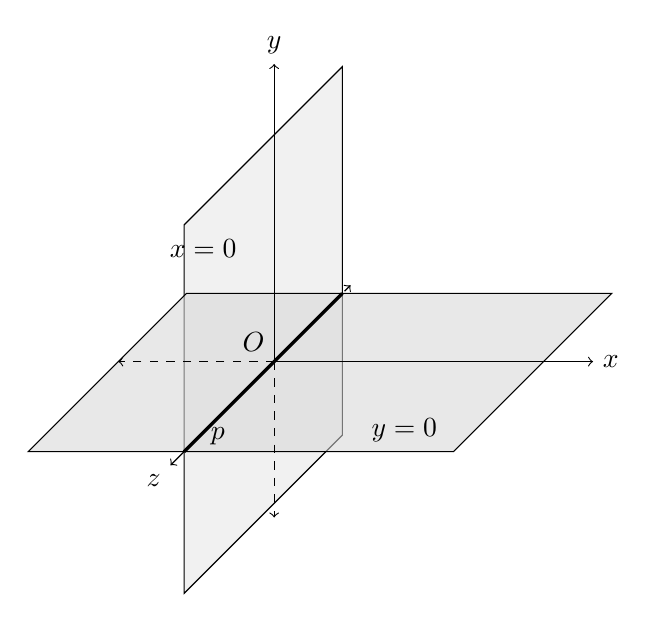
\begin{tikzpicture}[scale=0.9]

        % Rovina yz: x = 0
        \fill[gray!15, fill opacity=0.75]
            (0,-2,-2.5) -- (0,3.2,-2.5) --
            (0,3.2,3.3) -- (0,-2,3.3) -- cycle;
        \draw[thin]
            (0,-2,-2.5) -- (0,3.2,-2.5) --
            (0,3.2,3.3) -- (0,-2,3.3) -- cycle;

        % Rovina xz: y = 0
        \fill[gray!32, fill opacity=0.55]
            (-2.2,0,-2.5) -- (3.8,0,-2.5) --
            (3.8,0,3.3) -- (-2.2,0,3.3) -- cycle;
        \draw[thin]
            (-2.2,0,-2.5) -- (3.8,0,-2.5) --
            (3.8,0,3.3) -- (-2.2,0,3.3) -- cycle;

        % Osy - kladná část
        \draw[->] (0,0,0) -- (4.5,0,0) node[right] {$x$};
        \draw[->] (0,0,0) -- (0,4.2,0) node[above] {$y$};
        \draw[->] (0,0,0) -- (0,0,3.8) node[below left] {$z$};

        % Osy - záporná část
        \draw[->, dashed] (0,0,0) -- (-2.2,0,0);
        \draw[->, dashed] (0,0,0) -- (0,-2.2,0);
        \draw[->, dashed] (0,0,0) -- (0,0,-2.8);

        % Průsečnice rovin
        \draw[very thick] (0,0,-2.5) -- (0,0,3.3)
            node[pos=0.9, right] {$p$};

        \node[above left] at (0,0,0) {$O$};
        \node at (0,2.6,2.6) {$x=0$};
        \node at (2.8,0,2.5) {$y=0$};

    \end{tikzpicture}
    \caption{Osa $z$ je průsečnicí rovin $x=0$ a $y=0$.}
    \label{fig:Z_axis_as_intersection_of_planes}
\end{figure}

\begin{remark}
    Vyjádřením přímky jako průsečnice dvou rovin se nyní nebudeme
    podrobněji zabývat. Nejprve musíme poznat, jak lze roviny v prostoru
    popsat a jaké mohou mít vzájemné polohy. K tomuto způsobu vyjádření
    přímky se proto můžeme vrátit později.
\end{remark}

Tato úvaha nás přirozeně přivádí k dalšímu základnímu geometrickému
objektu v prostoru, kterým je rovina.


\subsection{Roviny v prostoru}
\label{subsec:Planes_in_space}

Rovina je nekonečný rovinný útvar, který se rozprostírá ve dvou navzájem
nezávislých směrech. Zatímco k určení přímky potřebujeme jeden bod a jeden
směr, k určení roviny potřebujeme jeden bod a dva různé směry, které
nejsou navzájem rovnoběžné.

Uvažujme bod
\[
    A[x_A;y_A;z_A]
\]
a dva nenulové, navzájem nerovnoběžné vektory
\[
    \vec{u}=(u_x;u_y;u_z),
    \qquad
    \vec{v}=(v_x;v_y;v_z).
\]
Vektory $\vec{u}$ a $\vec{v}$ určují dva směry ležící v rovině. Jejich
lineárními kombinacemi se můžeme z bodu $A$ dostat do libovolného dalšího
bodu této roviny.

\begin{figure}[H]
    \centering
    \begin{tikzpicture}[scale=0.9]

        % Rovina
        \coordinate (P1) at (-1,0,0.5);
        \coordinate (P2) at (3,1,0.5);
        \coordinate (P3) at (4,3,2.5);
        \coordinate (P4) at (0,2,2.5);

        \fill[gray!18] (P1) -- (P2) -- (P3) -- (P4) -- cycle;
        \draw[thin] (P1) -- (P2) -- (P3) -- (P4) -- cycle;

        % Osy - kladná část
        \draw[->] (0,0,0) -- (4.8,0,0) node[right] {$x$};
        \draw[->] (0,0,0) -- (0,4.3,0) node[above] {$y$};
        \draw[->] (0,0,0) -- (0,0,3.8) node[below left] {$z$};

        % Osy - záporná část
        \draw[->, dashed] (0,0,0) -- (-2.2,0,0);
        \draw[->, dashed] (0,0,0) -- (0,-2.2,0);
        \draw[->, dashed] (0,0,0) -- (0,0,-2.6);

        \node[above left] at (0,0,0) {$O$};

        % Bod a směrové vektory roviny
        \coordinate (A) at (1.4,1.3,1.3);
        \coordinate (U) at (3.8,1.9,1.3);
        \coordinate (V) at (2,2.5,2.5);

        \draw[vector] (A) -- (U)
            node[midway, sloped, above] {$\vec{u}$};
        \draw[vector] (A) -- (V)
            node[midway, sloped, above] {$\vec{v}$};

        \fill (A) circle (2pt) node[below left] {$A$};
        \node at (3.65,2.75,2.35) {$\alpha$};

    \end{tikzpicture}
    \caption{Rovina $\alpha$ určená bodem $A$ a dvěma navzájem
    nerovnoběžnými směrovými vektory $\vec{u}$ a $\vec{v}$.}
    \label{fig:Plane_point_two_vectors}
\end{figure}

Podobně jako přímku lze i rovinu určit několika různými způsoby. Rovinu
jednoznačně určují například:

\begin{itemize}
    \item jeden bod a dva navzájem nerovnoběžné směrové vektory;
    \item tři body, které neleží na jedné přímce;
    \item přímka a bod, který na této přímce neleží;
    \item dvě různoběžné přímky;
    \item dvě různé rovnoběžné přímky.
\end{itemize}

Podmínky uvedené v jednotlivých případech jsou důležité. Tři body ležící
na jedné přímce například rovinu jednoznačně neurčují, protože danou
přímkou prochází nekonečně mnoho rovin. Stejně tak dva rovnoběžné směrové
vektory určují pouze jeden směr, a nestačí proto k popsání celé roviny.

Roviny budeme popisovat dvěma základními způsoby:

\begin{itemize}
    \item \textbf{parametrickým vyjádřením}, které využívá jeden bod
    roviny a dva její směrové vektory;
    \item \textbf{obecnou rovnicí roviny}, která využívá normálový vektor
    kolmý k rovině.
\end{itemize}

Nejprve se zaměříme na parametrické vyjádření roviny, které přímo navazuje
na parametrické vyjádření přímky a na lineární kombinace vektorů.


\subsection{Parametrické vyjádření roviny}
\label{subsec:Parametric_plane}

Rovina je určena jedním bodem a dvěma navzájem nezávislými směry.
Z výchozího bodu se tedy můžeme pohybovat současně ve směru dvou
nenulových, navzájem nerovnoběžných vektorů.

Uvažujme bod
\[
    A[x_A;y_A;z_A]
\]
a dva nenulové, navzájem nerovnoběžné vektory
\[
    \vec{u}=(u_x;u_y;u_z),
    \qquad
    \vec{v}=(v_x;v_y;v_z).
\]

Libovolný bod $X[x;y;z]$ roviny získáme z bodu $A$ posunutím o vhodný
násobek vektoru $\vec{u}$ a vhodný násobek vektoru $\vec{v}$:
\[
    X=A+s\vec{u}+t\vec{v},
\]
kde $s,t\in\mathbb{R}$.


\subsubsection{Rovina určená bodem a dvěma směrovými vektory}
\label{subsubsec:Plane_point_two_direction_vectors}

\begin{definition}
    \label{def:Parametric_plane}

    Nechť $A[x_A;y_A;z_A]$ je bod v prostoru a nechť
    \[
        \vec{u}=(u_x;u_y;u_z),
        \qquad
        \vec{v}=(v_x;v_y;v_z)
    \]
    jsou dva nenulové, navzájem nerovnoběžné vektory.

    Rovina $\alpha$ procházející bodem $A$ a mající směrové vektory
    $\vec{u}$ a $\vec{v}$ je množina všech bodů $X$, které lze vyjádřit
    ve tvaru
    \begin{equation}
        X=A+s\vec{u}+t\vec{v},
        \qquad
        s,t\in\mathbb{R}.
        \label{eq:Parametric_plane_vector}
    \end{equation}

    Po rozepsání do souřadnic získáme parametrické rovnice roviny
    \begin{equation}
        \begin{aligned}
            \alpha: x&=x_A+s u_x+t v_x,\\
            y&=y_A+s u_y+t v_y,\\
            z&=z_A+s u_z+t v_z; \quad s,t\in\mathbb{R}.
        \end{aligned}
        \label{eq:Parametric_plane_coordinates}
    \end{equation}

    Parametry $s$ a $t$ jsou opět známými \textbf{parametry roviny} a vektory
    $\vec{u}$ a $\vec{v}$ jejími \textbf{směrovými vektory}.
\end{definition}

Vektor směřující z bodu $A$ do libovolného bodu $X$ roviny má tvar
\begin{equation}
    \overrightarrow{AX}=s\vec{u}+t\vec{v}.
    \label{eq:Plane_displacement_vector}
\end{equation}

Každý vektor spojující bod $A$ s bodem roviny je tedy lineární kombinací
jejích směrových vektorů.

\begin{figure}[H]
    \centering
    \begin{tikzpicture}[scale=0.9]

        % Rovina
        \coordinate (P1) at (-1.2,0.1,0.3);
        \coordinate (P2) at (4.4,1.2,0.9);
        \coordinate (P3) at (5.0,3.8,2.9);
        \coordinate (P4) at (-0.6,2.7,2.3);

        \fill[gray!18] (P1) -- (P2) -- (P3) -- (P4) -- cycle;
        \draw[thin] (P1) -- (P2) -- (P3) -- (P4) -- cycle;

        % Osy - kladná část
        \draw[->] (0,0,0) -- (5.2,0,0) node[right] {$x$};
        \draw[->] (0,0,0) -- (0,4.7,0) node[above] {$y$};
        \draw[->] (0,0,0) -- (0,0,4.1) node[below left] {$z$};

        % Osy - záporná část
        \draw[->, dashed] (0,0,0) -- (-2.2,0,0);
        \draw[->, dashed] (0,0,0) -- (0,-2.2,0);
        \draw[->, dashed] (0,0,0) -- (0,0,-2.7);

        \node[above left] at (0,0,0) {$O$};

        % Body
        \coordinate (A) at (1,1,1);
        \coordinate (U) at (3,1.4,1.2);
        \coordinate (V) at (1.6,2.4,2);
        \coordinate (X) at (3.6,2.8,2.2);

        % Směrové vektory
        \draw[vector] (A) -- (U)
            node[midway, sloped, above] {$\vec{u}$};

        \draw[vector] (A) -- (V)
            node[midway, sloped, above] {$\vec{v}$};

        % Pomocný rovnoběžník
        \draw[dashed] (U) -- (X);
        \draw[dashed] (V) -- (X);

        % Body
        \fill (A) circle (2pt) node[below left] {$A$};
        \fill (X) circle (2pt) node[above right] {$X$};

        \node at (4.35,3,2.65) {$\alpha$};

    \end{tikzpicture}

    \caption{Bod $X$ roviny $\alpha$ získáme z bodu $A$ posunutím
    ve směrech vektorů $\vec{u}$ a $\vec{v}$.}
    \label{fig:Parametric_plane_geometric_meaning}
\end{figure}

Na obrázku~\ref{fig:Parametric_plane_geometric_meaning} je znázorněn
geometrický význam vztahu~\eqref{eq:Parametric_plane_vector}.
Posunutí
\[
    s\vec{u}+t\vec{v}
\]
může mít libovolnou velikost i orientaci v rámci roviny určené směry
$\vec{u}$ a $\vec{v}$.


\subsubsection{Význam parametrů}
\label{subsubsec:Meaning_of_plane_parameters}

Parametry $s$ a $t$ se mohou měnit nezávisle na sobě. Každá uspořádaná
dvojice
\[
    (s;t)\in\mathbb{R}^2
\]
určuje právě jeden bod roviny.

Pro některé zvláštní hodnoty parametrů dostáváme:

\begin{itemize}
    \item pro $s=0$ a $t=0$ získáme výchozí bod
    \[
        X=A;
    \]

    \item pro $t=0$ se pohybujeme pouze ve směru vektoru $\vec{u}$:
    \[
        X=A+s\vec{u},
    \]
    dostáváme tím tedy přímku procházející bodem $A$ a rovnoběžnou s vektorem $\vec{u}$;

    \item pro $s=0$ se pohybujeme pouze ve směru vektoru $\vec{v}$:
    \[
        X=A+t\vec{v},
    \]
    dostáváme tím tedy přímku procházející bodem $A$ a rovnoběžnou s vektorem $\vec{v}$;

    \item pro pevně zvolené $t$ a proměnné $s$ získáváme přímku
    rovnoběžnou s vektorem $\vec{u}$;

    \item pro pevně zvolené $s$ a proměnné $t$ získáváme přímku
    rovnoběžnou s vektorem $\vec{v}$.
\end{itemize}

Rovinu si tak můžeme představit jako nekonečnou soustavu navzájem
rovnoběžných přímek. Například při pevně zvoleném parametru $t$
a proměnném parametru $s$ získáváme přímky rovnoběžné se směrovým
vektorem $\vec{u}$, jejichž sjednocením je celá rovina.

\begin{remark}
    Pro parametrické vyjádření přímky stačil jeden parametr, protože
    přímka má pouze jeden nezávislý směr. Rovina má dva nezávislé
    směry, a proto potřebujeme dva parametry.
\end{remark}


\subsubsection{Proč musí být směrové vektory nerovnoběžné}
\label{subsubsec:Why_plane_vectors_nonparallel}

Podmínka, že vektory $\vec{u}$ a $\vec{v}$ nejsou rovnoběžné, je
nezbytná.

Kdyby například existovalo číslo $k\in\mathbb{R}$ takové, že
\[
    \vec{v}=k\vec{u},
\]
potom by platilo
\begin{align*}
    X
    &=A+s\vec{u}+t\vec{v}\\
    &=A+s\vec{u}+tk\vec{u}\\
    &=A+(s+kt)\vec{u}.
\end{align*}

Místo dvou nezávislých směrů bychom tedy získali pouze násobky jediného
vektoru $\vec{u}$. Výslednou množinou bodů by nebyla rovina, ale přímka.

Podobný problém nastane, pokud je některý ze směrových vektorů nulový.
Nulový vektor neurčuje žádný směr a jeho násobky nemění polohu bodu.

\begin{remark}
    Dva vektory mohou tvořit dvojici směrových vektorů roviny právě
    tehdy, jsou-li lineárně nezávislé. Pro dvojici vektorů to znamená,
    že ani jeden z nich není reálným násobkem druhého.
\end{remark}


\subsubsection{Sestavení parametrického vyjádření roviny}
\label{subsubsec:Constructing_parametric_plane}

Při sestavování parametrického vyjádření roviny potřebujeme:

\begin{enumerate}
    \item jeden bod $A$, který v rovině leží;
    \item dva nenulové, navzájem nerovnoběžné směrové vektory
    $\vec{u}$ a $\vec{v}$ ležící v rovině;
    \item dosadit tyto údaje do vztahu
    \[
        X=A+s\vec{u}+t\vec{v}.
    \]
\end{enumerate}

\begin{example}
    \label{exa:Parametric_plane_point_vectors}

    Určete parametrické vyjádření roviny $\alpha$, která prochází bodem
    $A[1;-2;3]$ a má směrové vektory $\vec{u}=(2;1;-1)\text{, } \vec{v}=(1;-1;2)$.

    Vektory $\vec{u}$ a $\vec{v}$ nejsou rovnoběžné, a proto určují
    dva nezávislé směry roviny.

    Použijeme vztah~\eqref{eq:Parametric_plane_vector}:
    \begin{align*}
        X
        &=A+s\vec{u}+t\vec{v}\\
        &=[1;-2;3]+s(2;1;-1)+t(1;-1;2)\\
        &=[1+2s+t;-2+s-t;3-s+2t].
    \end{align*}

    Parametrické vyjádření roviny je
    \[
        \begin{aligned}
            \alpha: x&=1+2s+t,\\
            y&=-2+s-t,\\
            z&=3-s+2t; \quad s,t\in\mathbb{R}.
        \end{aligned}
    \]
\end{example}

Z parametrického vyjádření můžeme vytvářet jednotlivé body roviny
volbou konkrétních hodnot parametrů. Pro rovinu z předchozího příkladu
například dostáváme

\[
    \begin{array}{c|c|c}
        s & t & X[x;y;z]\\
        \hline
        0 & 0 & A[1;-2;3]\\
        1 & 0 & B[3;-1;2]\\
        0 & 1 & C[2;-3;5]\\
        1 & 1 & D[4;-2;4]
    \end{array}
\]

Body $A$, $B$, $C$ a $D$ tvoří rovnoběžník. Platí totiž
\[
    \overrightarrow{AB}=\vec{u},
    \qquad
    \overrightarrow{AC}=\vec{v},
\]
a bod $D$ získáme současným posunutím o oba směrové vektory:
\[
    D=A+\vec{u}+\vec{v}.
\]


\subsubsection{Čtení parametrického vyjádření roviny}
\label{subsubsec:Reading_parametric_plane}

Z parametrických rovnic můžeme přímo vyčíst jeden bod roviny a dva
její směrové vektory. Konstantní členy určují bod odpovídající hodnotám
$s=0$, $t=0$. Koeficienty u parametru $s$ tvoří souřadnice prvního
směrového vektoru a koeficienty u parametru $t$ souřadnice druhého.

\begin{example}
    \label{exa:Reading_parametric_plane}

    Je dána rovina
    \[
        \begin{aligned}
            \beta: x&=-1+3s-t,\\
            y&=2-s+2t,\\
            z&=4+2s+t; \quad s,t\in\mathbb{R}.
        \end{aligned}
    \]

    Určete jeden bod roviny a dva její směrové vektory.

    Pro $s=0$ a $t=0$ dostáváme bod
    \[
        K[-1;2;4].
    \]

    Koeficienty u parametru $s$ tvoří směrový vektor
    \[
        \vec{u}=(3;-1;2),
    \]
    zatímco koeficienty u parametru $t$ tvoří druhý směrový vektor
    \[
        \vec{v}=(-1;2;1).
    \]

    Rovina $\beta$ tedy prochází bodem $K[-1;2;4]$ a má směrové vektory
    \[
        \vec{u}=(3;-1;2),
        \qquad
        \vec{v}=(-1;2;1).
    \]
\end{example}

Při čtení směrových vektorů je třeba dávat pozor zejména na znaménka.
Například z rovnice
\[
    y=2-s+2t
\]
čteme jako druhou souřadnici prvního směrového vektoru číslo $-1$
a jako druhou souřadnici druhého směrového vektoru číslo $2$.


\subsubsection{Příslušnost bodu k rovině}
\label{subsubsec:Point_membership_parametric_plane}

Aby bod $P[x_P;y_P;z_P]$ ležel v parametricky vyjádřené rovině,
musí existovat jedna dvojice reálných parametrů $(s;t)$, která
současně vytvoří všechny tři souřadnice bodu $P$.

Pro rovinu
\[
    \begin{aligned}
        \alpha: x&=x_A+s u_x+t v_x,\\
        y&=y_A+s u_y+t v_y,\\
        z&=z_A+s u_z+t v_z; \quad s,t\in\mathbb{R}
    \end{aligned}
\]
tedy platí
\[
    P\in\alpha
    \quad\Longleftrightarrow\quad
    \text{existují }s,t\in\mathbb{R}\text{ takové, že}
    \begin{cases}
        x_P=x_A+s u_x+t v_x,\\
        y_P=y_A+s u_y+t v_y,\\
        z_P=z_A+s u_z+t v_z.
    \end{cases}
\]

Nestačí, aby některé dvě rovnice určily dvojici parametrů. Stejná
dvojice hodnot $s$ a $t$ musí splňovat všechny tři rovnice.

\begin{example}
    \label{exa:Point_membership_parametric_plane}

    Rozhodněte, zda body
    \[
        P[4;-2;4],
        \qquad
        Q[3;-1;3]
    \]
    leží v rovině
    \[
        \begin{aligned}
            \alpha: x&=1+2s+t,\\
            y&=-2+s-t,\\
            z&=3-s+2t; \quad s,t\in\mathbb{R}.
        \end{aligned}
    \]

    Nejprve dosadíme souřadnice bodu $P[4;-2;4]$:
    \[
        \begin{cases}
            4=1+2s+t,\\
            -2=-2+s-t,\\
            4=3-s+2t.
        \end{cases}
    \]

    Po úpravě
    \[
        \begin{cases}
            2s+t=3,\\
            s-t=0,\\
            -s+2t=1.
        \end{cases}
    \]

    Z druhé rovnice plyne
    \[
        s=t.
    \]

    Po dosazení do první rovnice získáme
    \[
        3s=3,
    \]
    tedy
    \[
        s=1,
        \qquad
        t=1.
    \]

    Ověříme třetí rovnici:
    \[
        -1+2\cdot1=1.
    \]

    Stejná dvojice parametrů $(s;t)=(1;1)$ splňuje všechny tři
    rovnice, a proto
    \[
        P\in\alpha.
    \]

    Nyní dosadíme souřadnice bodu $Q[3;-1;3]$:
    \[
        \begin{cases}
            3=1+2s+t,\\
            -1=-2+s-t,\\
            3=3-s+2t.
        \end{cases}
    \]

    Po úpravě
    \[
        \begin{cases}
            2s+t=2,\\
            s-t=1,\\
            -s+2t=0.
        \end{cases}
    \]

    Z prvních dvou rovnic dostáváme
    \[
        s=1,
        \qquad
        t=0.
    \]

    Tato dvojice však nesplňuje třetí rovnici, protože
    \[
        -1+2\cdot0=-1\neq0.
    \]

    Proto
    \[
        Q\notin\alpha.
    \]
\end{example}

Příslušnost bodu můžeme vyjádřit také vektorově. Bod $P$ leží
v rovině procházející bodem $A$ se směrovými vektory $\vec{u}$
a $\vec{v}$ právě tehdy, když lze vektor
\[
    \overrightarrow{AP}=P-A
\]
vyjádřit jako lineární kombinaci
\[
    \overrightarrow{AP}=s\vec{u}+t\vec{v}
\]
pro nějaká $s,t\in\mathbb{R}$.


\subsubsection{Rovina určená třemi body}
\label{subsubsec:Plane_through_three_points}

Rovina bývá často zadána třemi body
\[
    A[x_A;y_A;z_A],
    \qquad
    B[x_B;y_B;z_B],
    \qquad
    C[x_C;y_C;z_C].
\]

Aby tyto body určovaly právě jednu rovinu, nesmějí ležet na jedné
přímce.

Jako výchozí bod můžeme zvolit například bod $A$. Dva směrové vektory
roviny získáme jako
\[
    \overrightarrow{AB}
    =
    (x_B-x_A;y_B-y_A;z_B-z_A)
\]
a
\[
    \overrightarrow{AC}
    =
    (x_C-x_A;y_C-y_A;z_C-z_A).
\]

Pokud body $A$, $B$ a $C$ neleží na jedné přímce, nejsou vektory
$\overrightarrow{AB}$ a $\overrightarrow{AC}$ rovnoběžné a mohou
sloužit jako směrové vektory roviny.

Parametrické vyjádření potom má tvar
\begin{equation}
    X=A+s\overrightarrow{AB}+t\overrightarrow{AC},
    \qquad
    s,t\in\mathbb{R}.
    \label{eq:Plane_through_three_points}
\end{equation}

Po rozepsání do souřadnic:
\begin{equation}
    \begin{aligned}
        \alpha: x&=x_A+s(x_B-x_A)+t(x_C-x_A),\\
        y&=y_A+s(y_B-y_A)+t(y_C-y_A),\\
        z&=z_A+s(z_B-z_A)+t(z_C-z_A);
        \quad s,t\in\mathbb{R}.
    \end{aligned}
    \label{eq:Plane_through_three_points_coordinates}
\end{equation}

\begin{example}
    \label{exa:Plane_through_three_points}

    Určete parametrické vyjádření roviny $\alpha$, která prochází body
    \[
        A[1;-2;3],
        \qquad
        B[3;-1;2],
        \qquad
        C[2;-3;5].
    \]

    Jako výchozí bod zvolíme bod $A$. Určíme vektory
    \[
        \overrightarrow{AB}
        =
        (3-1;-1-(-2);2-3)
        =
        (2;1;-1)
    \]
    a
    \[
        \overrightarrow{AC}
        =
        (2-1;-3-(-2);5-3)
        =
        (1;-1;2).
    \]

    Vektory $\overrightarrow{AB}$ a $\overrightarrow{AC}$ nejsou
    rovnoběžné, takže zadané body neleží na jedné přímce a určují
    právě jednu rovinu.

    Parametrické vyjádření roviny je
    \[
        \begin{aligned}
            \alpha: x&=1+2s+t,\\
            y&=-2+s-t,\\
            z&=3-s+2t; \quad s,t\in\mathbb{R}.
        \end{aligned}
    \]
\end{example}

\begin{remark}
    Jako výchozí bod nemusíme zvolit právě bod $A$. Můžeme použít
    také bod $B$ nebo $C$ a vytvořit dva vhodné vektory vycházející
    z tohoto bodu. Výsledné parametrické vyjádření bude vypadat jinak,
    ale bude popisovat tutéž rovinu.
\end{remark}

Pokud by byly vektory $\overrightarrow{AB}$ a $\overrightarrow{AC}$
rovnoběžné, ležely by body $A$, $B$ a $C$ na jedné přímce. Takovými
třemi body prochází nekonečně mnoho rovin, a proto by rovina nebyla
určena jednoznačně.


\subsubsection{Rovina určená přímkou a bodem}
\label{subsubsec:Plane_line_and_point}

Rovinu lze jednoznačně určit také přímkou $p$ a bodem $C$, který
na této přímce neleží.

Nechť je přímka zadána parametricky ve tvaru
\[
    X=A+r\vec{u},
    \qquad
    r\in\mathbb{R}.
\]

Jeden směrový vektor roviny získáme přímo z přímky:
\[
    \vec{u}.
\]

Druhý směrový vektor vytvoříme spojením bodu $A$ přímky s bodem $C$:
\[
    \overrightarrow{AC}=C-A.
\]

Protože bod $C$ na přímce neleží, nejsou vektory $\vec{u}$ a
$\overrightarrow{AC}$ rovnoběžné.

Parametrické vyjádření roviny má tedy tvar
\begin{equation}
    X=A+s\vec{u}+t\overrightarrow{AC},
    \qquad
    s,t\in\mathbb{R}.
    \label{eq:Plane_line_and_point}
\end{equation}

\begin{example}
    \label{exa:Plane_line_and_point}

    Určete parametrické vyjádření roviny $\alpha$, která obsahuje přímku
    \[
        \begin{aligned}
            p: x&=1+2r,\\
            y&=-2+r,\\
            z&=3-r; \quad r\in\mathbb{R}
        \end{aligned}
    \]
    a bod
    \[
        C[2;-3;5].
    \]

    Z parametrického vyjádření přímky vyčteme bod
    \[
        A[1;-2;3]
    \]
    a její směrový vektor
    \[
        \vec{u}=(2;1;-1).
    \]

    Druhý směrový vektor roviny získáme jako
    \[
        \overrightarrow{AC}
        =
        (2-1;-3-(-2);5-3)
        =
        (1;-1;2).
    \]

    Parametrické vyjádření roviny je
    \[
        \begin{aligned}
            \alpha: x&=1+2s+t,\\
            y&=-2+s-t,\\
            z&=3-s+2t; \quad s,t\in\mathbb{R}.
        \end{aligned}
    \]
\end{example}

\begin{remark}
    Kdyby bod $C$ ležel na přímce $p$, byl by vektor
    $\overrightarrow{AC}$ rovnoběžný se směrovým vektorem přímky.
    Získali bychom pouze jeden nezávislý směr a rovina by nebyla
    určena jednoznačně. Danou přímkou totiž prochází nekonečně mnoho
    rovin.
\end{remark}


\subsubsection{Rovina určená dvěma přímkami}
\label{subsubsec:Plane_determined_by_two_lines}

Dvě přímky určují rovinu pouze v některých případech.

\paragraph{Dvě různoběžné přímky.}

Jestliže se přímky $p$ a $q$ protínají v bodě $A$ a mají navzájem
nerovnoběžné směrové vektory $\vec{u}$ a $\vec{v}$, určují právě
jednu rovinu:
\[
    X=A+s\vec{u}+t\vec{v},
    \qquad
    s,t\in\mathbb{R}.
\]

\begin{example}
    \label{exa:Plane_two_intersecting_lines}

    Určete parametrické vyjádření roviny $\alpha$, která obsahuje
    přímky
    \[
        \begin{aligned}
            p: x&=1+r,\\
            y&=2-r,\\
            z&=3+2r; \quad r\in\mathbb{R}
        \end{aligned}
    \]
    a
    \[
        \begin{aligned}
            q: x&=1+2s,\\
            y&=2+s,\\
            z&=3-s; \quad s\in\mathbb{R}.
        \end{aligned}
    \]

    Pro $r=0$ a $s=0$ získáváme u obou přímek bod
    \[
        A[1;2;3].
    \]

    Přímky se tedy protínají v bodě $A$.

    Jejich směrové vektory jsou
    \[
        \vec{u}=(1;-1;2),
        \qquad
        \vec{v}=(2;1;-1).
    \]

    Vektory nejsou rovnoběžné, proto přímky určují právě jednu rovinu.

    Její parametrické vyjádření je
    \[
        X=A+k\vec{u}+l\vec{v},
    \]
    tedy
    \[
        \begin{aligned}
            \alpha: x&=1+k+2l,\\
            y&=2-k+l,\\
            z&=3+2k-l; \quad k,l\in\mathbb{R}.
        \end{aligned}
    \]
\end{example}

\paragraph{Dvě různé rovnoběžné přímky.}

Nechť přímky mají společný směrový vektor $\vec{u}$. Zvolíme bod $A$
na první přímce a bod $B$ na druhé přímce. Druhý směr roviny určí
vektor
\[
    \overrightarrow{AB}.
\]

Protože jsou přímky různé, není vektor $\overrightarrow{AB}$
rovnoběžný s vektorem $\vec{u}$. Rovina má parametrické vyjádření
\[
    X=A+s\vec{u}+t\overrightarrow{AB},
    \qquad
    s,t\in\mathbb{R}.
\]

\paragraph{Dvě mimoběžné přímky.}

Mimoběžné přímky neleží v jedné rovině. Žádná rovina je proto nemůže
současně obsahovat.

\begin{remark}
    Dvě přímky určují právě jednu rovinu tehdy, jsou-li různoběžné
    nebo jsou-li různé a rovnoběžné. Mimoběžné přímky společnou
    rovinu nemají a dvě totožné přímky leží v nekonečně mnoha rovinách.
\end{remark}


\subsubsection{Nejednoznačnost parametrického vyjádření roviny}
\label{subsubsec:Nonuniqueness_parametric_plane}

Stejně jako parametrické vyjádření přímky není ani parametrické
vyjádření roviny jednoznačné.

Pro tutéž rovinu můžeme zvolit:

\begin{itemize}
    \item libovolný její bod jako výchozí bod;
    \item libovolné dva lineárně nezávislé vektory ležící v této
    rovině jako směrové vektory;
    \item jiná označení parametrů.
\end{itemize}

Uvažujme rovinu
\[
    X=A+s\vec{u}+t\vec{v},
\]
kde
\[
    A[1;-2;3],
    \qquad
    \vec{u}=(2;1;-1),
    \qquad
    \vec{v}=(1;-1;2).
\]

Bod
\[
    B=A+\vec{u}=[3;-1;2]
\]
v této rovině leží.

Také vektor
\[
    \vec{w}
    =
    \vec{u}+\vec{v}
    =
    (3;0;1)
\]
je směrovým vektorem této roviny. Vektory $\vec{u}$ a $\vec{w}$
nejsou rovnoběžné, takže tutéž rovinu můžeme zapsat například jako
\[
    X=B+r\vec{u}+q\vec{w},
    \qquad
    r,q\in\mathbb{R}.
\]

Po rozepsání:
\[
    \begin{aligned}
        \alpha: x&=3+2r+3q,\\
        y&=-1+r,\\
        z&=2-r+q; \quad r,q\in\mathbb{R}.
    \end{aligned}
\]

Oba zápisy popisují tutéž rovinu, přestože používají jiný výchozí bod,
jinou dvojici směrových vektorů i jiná označení parametrů.

Skutečně platí
\begin{align*}
    B+r\vec{u}+q\vec{w}
    &=
    A+\vec{u}+r\vec{u}+q(\vec{u}+\vec{v})\\
    &=
    A+(1+r+q)\vec{u}+q\vec{v}.
\end{align*}

Každý bod druhého vyjádření je tedy bodem prvního vyjádření. Protože
hodnoty $1+r+q$ a $q$ mohou nabývat libovolných reálných hodnot, platí
také opačné tvrzení.

\begin{remark}
    Dva různé parametrické zápisy mohou popisovat tutéž rovinu.
    Nestačí proto porovnávat pouze výchozí body nebo jednotlivé
    směrové vektory. Rozhodující je, zda oba zápisy popisují stejnou
    množinu bodů a stejné dva nezávislé směry v prostoru.
\end{remark}


% ============================================================
%             P Ř E C H O D   K   O B E C N É   R O V N I C I
% ============================================================

Parametrické vyjádření roviny využívá dva navzájem nezávislé směry,
které v rovině leží. Rovinu však můžeme popsat také opačným způsobem:
pomocí směru, který je k celé rovině kolmý.

Má-li rovina směrové vektory
\[
    \vec{u}
    \qquad\text{a}\qquad
    \vec{v},
\]
potom jejich vektorový součin
\[
    \vec{n}
    =
    \vec{u}\times\vec{v}
\]
je kolmý současně k oběma směrovým vektorům, a tedy k celé rovině.

\begin{definition}
    Nenulový vektor $\vec{n}$ kolmý k rovině nazýváme
    \textbf{normálovým vektorem roviny}.
\end{definition}

Je-li
\[
    \vec{n}=(a;b;c),
\]
potom právě jeho souřadnice budou hrát zásadní roli při zápisu roviny
pomocí její \textbf{obecné rovnice}, kterou se budeme zabývat
v následující podkapitole.
\subsection{Obecná rovnice roviny}
\label{subsec:General_plane_equation}

V předchozí části jsme rovinu popisovali pomocí jednoho jejího bodu,
dvou směrových vektorů a dvou parametrů. Změnou parametrů jsme vytvářeli
jednotlivé body roviny. Parametrické vyjádření nám tedy říká,
\emph{jak body roviny získávat}.

Rovinu však můžeme popsat také jedinou rovnicí o třech proměnných $x$,
$y$ a $z$, kterou splňují právě souřadnice bodů ležících v této rovině.
Takový zápis umožňuje například rychle ověřit, zda daný bod v rovině leží,
nebo snadno porovnávat směry různých rovin. Tento způsob popisu nazýváme
\textbf{obecnou rovnicí roviny}.

Základní roli při jejím odvození bude hrát vektor, který je k rovině kolmý.

\subsubsection{Normálový vektor roviny}
\label{subsubsec:Normal_vector_plane}

Při parametrickém vyjádření roviny jsme její směry určovali pomocí dvou
navzájem nerovnoběžných směrových vektorů. Nyní budeme místo nich pracovat
s vektorem, který je kolmý ke všem směrům ležícím v rovině.

\begin{definition}
    \label{def:Normal_vector_plane}
    \textbf{Normálovým vektorem roviny} $\alpha$ nazýváme každý nenulový
    vektor $\vec{n}$, který je kolmý k této rovině.
\end{definition}

Je-li rovina $\alpha$ určena dvěma směrovými vektory $\vec{u}$ a
$\vec{v}$ a je-li $\vec{n}$ jejím normálovým vektorem, potom platí
\begin{equation}
    \vec{n}\cdot\vec{u}=0
    \qquad\text{a}\qquad
    \vec{n}\cdot\vec{v}=0.
    \label{eq:Normal_vector_plane_orthogonality}
\end{equation}

Normálový vektor je tedy kolmý k oběma nezávislým směrům roviny. Protože
každý další směrový vektor roviny vznikne jako lineární kombinace
$\vec{u}$ a $\vec{v}$, je normálový vektor kolmý také ke každému dalšímu
vektoru ležícímu v rovině.

Známe-li dva navzájem nerovnoběžné směrové vektory roviny, můžeme
normálový vektor určit pomocí jejich vektorového součinu:
\begin{equation}
    \vec{n}=\vec{u}\times\vec{v}.
    \label{eq:Normal_vector_plane_cross_product}
\end{equation}

Vektorový součin je kolmý k oběma násobeným vektorům, a proto je kolmý
také k rovině, kterou tyto vektory určují.

\begin{figure}[H]
    \centering
    \begin{tikzpicture}[scale=0.9]

        % Rovina
        \coordinate (P1) at (-1.3,0.1,0.2);
        \coordinate (P2) at (4.3,1.2,0.8);
        \coordinate (P3) at (5.0,3.7,2.8);
        \coordinate (P4) at (-0.6,2.6,2.2);

        \fill[gray!18] (P1) -- (P2) -- (P3) -- (P4) -- cycle;
        \draw[thin] (P1) -- (P2) -- (P3) -- (P4) -- cycle;

        % Osy - kladná část
        \draw[->] (0,0,0) -- (5.2,0,0) node[right] {$x$};
        \draw[->] (0,0,0) -- (0,4.6,0) node[above] {$y$};
        \draw[->] (0,0,0) -- (0,0,4.2) node[below left] {$z$};

        % Osy - záporná část
        \draw[->, dashed] (0,0,0) -- (-2.2,0,0);
        \draw[->, dashed] (0,0,0) -- (0,-2.2,0);
        \draw[->, dashed] (0,0,0) -- (0,0,-2.7);

        \node[above left] at (0,0,0) {$O$};

        % Bod a vektory
        \coordinate (A) at (1.4,1.3,1.3);
        \coordinate (U) at (3.6,1.75,1.5);
        \coordinate (V) at (2.0,2.65,2.3);
        \coordinate (N) at (1.4,2.0,3.7);

        \draw[vector] (A) -- (U)
            node[midway, sloped, above] {$\vec{u}$};
        \draw[vector] (A) -- (V)
            node[midway, sloped, above] {$\vec{v}$};
        \draw[vector] (A) -- (N)
            node[midway, right] {$\vec{n}$};

        % Naznačení pravého úhlu
        \draw
            (1.62,1.43,1.42)
            -- (1.58,1.61,1.63)
            -- (1.36,1.51,1.57);

        \fill (A) circle (2pt) node[below left] {$A$};
        \node at (4.25,3.1,2.55) {$\alpha$};

    \end{tikzpicture}
    \caption{Směrové vektory $\vec{u}$ a $\vec{v}$ leží v rovině
    $\alpha$, zatímco normálový vektor $\vec{n}$ je k rovině kolmý.}
    \label{fig:Normal_vector_plane}
\end{figure}

Stejně jako směrové vektory ani normálový vektor není určen jednoznačně.
Je-li $\vec{n}$ normálovým vektorem roviny, potom je jejím normálovým
vektorem také každý jeho nenulový reálný násobek
\[
    k\vec{n},
    \qquad
    k\in\mathbb{R}\setminus\{0\}.
\]
Všechny tyto vektory jsou navzájem rovnoběžné a jsou kolmé k téže rovině.

\subsubsection{Odvození obecné rovnice roviny}
\label{subsubsec:Derivation_general_plane_equation}

Uvažujme rovinu $\alpha$, která prochází bodem
\[
    A[x_A;y_A;z_A]
\]
a má normálový vektor
\[
    \vec{n}=(a;b;c),
\]
kde alespoň jedna ze souřadnic $a$, $b$, $c$ je nenulová. Dále zvolme
libovolný bod prostoru
\[
    X[x;y;z].
\]

Vektor směřující z bodu $A$ do bodu $X$ má souřadnice
\[
    \overrightarrow{AX}
    =(x-x_A;y-y_A;z-z_A).
\]

Bod $X$ leží v rovině $\alpha$ právě tehdy, když vektor
$\overrightarrow{AX}$ leží ve směru této roviny. Proto musí být kolmý
k normálovému vektoru $\vec{n}$. Pomocí skalárního součinu tuto podmínku
zapíšeme jako
\begin{equation}
    \vec{n}\cdot\overrightarrow{AX}=0.
    \label{eq:Point_normal_condition_plane}
\end{equation}

Po dosazení souřadnic obou vektorů dostáváme
\begin{align*}
    (a;b;c)\cdot(x-x_A;y-y_A;z-z_A)&=0,\\
    a(x-x_A)+b(y-y_A)+c(z-z_A)&=0.
\end{align*}

Rovnice
\begin{equation}
    a(x-x_A)+b(y-y_A)+c(z-z_A)=0
    \label{eq:Point_normal_plane_equation}
\end{equation}
popisuje rovinu, která prochází bodem $A[x_A;y_A;z_A]$ a má normálový
vektor $\vec{n}=(a;b;c)$. Tento zápis můžeme nazývat
\textbf{bodově-normálovým tvarem rovnice roviny}.

\begin{figure}[H]
    \centering
    \begin{tikzpicture}[scale=0.9]

        % Rovina
        \coordinate (P1) at (-1.3,0.1,0.2);
        \coordinate (P2) at (4.3,1.2,0.8);
        \coordinate (P3) at (5.0,3.7,2.8);
        \coordinate (P4) at (-0.6,2.6,2.2);

        \fill[gray!18] (P1) -- (P2) -- (P3) -- (P4) -- cycle;
        \draw[thin] (P1) -- (P2) -- (P3) -- (P4) -- cycle;

        % Osy - kladná část
        \draw[->] (0,0,0) -- (5.2,0,0) node[right] {$x$};
        \draw[->] (0,0,0) -- (0,4.6,0) node[above] {$y$};
        \draw[->] (0,0,0) -- (0,0,4.2) node[below left] {$z$};

        % Osy - záporná část
        \draw[->, dashed] (0,0,0) -- (-2.2,0,0);
        \draw[->, dashed] (0,0,0) -- (0,-2.2,0);
        \draw[->, dashed] (0,0,0) -- (0,0,-2.7);

        \node[above left] at (0,0,0) {$O$};

        % Body
        \coordinate (A) at (1.2,1.2,1.2);
        \coordinate (X) at (3.7,2.5,2.1);
        \coordinate (Y) at (3.1,2.1,3.5);
        \coordinate (N) at (1.2,1.9,3.6);

        \fill (A) circle (2pt) node[below left] {$A$};
        \fill (X) circle (2pt) node[below right] {$X$};
        \fill (Y) circle (2pt) node[above right] {$Y$};

        % Vektory
        \draw[vector] (A) -- (X)
            node[midway, sloped, below] {$\overrightarrow{AX}$};
        \draw[vector] (A) -- (N)
            node[midway, right] {$\vec{n}$};
        \draw[vector, dashed] (A) -- (Y)
            node[midway, sloped, above] {$\overrightarrow{AY}$};

        % Bod Y mimo rovinu
        \draw[dashed] (Y) -- (2.8,1.85,2.6);

        \node at (4.25,3.1,2.55) {$\alpha$};

    \end{tikzpicture}
    \caption{Bod $X$ leží v rovině $\alpha$, protože vektor
    $\overrightarrow{AX}$ je kolmý k normálovému vektoru $\vec{n}$.
    U bodu $Y$, který v rovině neleží, tato kolmost neplatí.}
    \label{fig:General_plane_derivation}
\end{figure}

Roznásobením rovnice~\eqref{eq:Point_normal_plane_equation} získáme
\begin{align*}
    a(x-x_A)+b(y-y_A)+c(z-z_A)&=0,\\
    ax-ax_A+by-by_A+cz-cz_A&=0,\\
    ax+by+cz-(ax_A+by_A+cz_A)&=0.
\end{align*}

Bod $A$ i normálový vektor $\vec{n}$ jsou pevně zvolené, a proto je
výraz
\[
    -(ax_A+by_A+cz_A)
\]
konstantou. Označíme-li tuto konstantu písmenem $d$, dostáváme rovnici
\[
    ax+by+cz+d=0.
\]

\begin{definition}
    \label{def:General_plane_equation}
    \textbf{Obecnou rovnicí roviny} v prostoru nazýváme rovnici tvaru
    \begin{equation}
        ax+by+cz+d=0,
        \label{eq:General_plane_equation}
    \end{equation}
    kde
    \[
        a,b,c,d\in\mathbb{R}
        \qquad\text{a}\qquad
        (a;b;c)\neq(0;0;0).
    \]

    Rovina $\alpha$ je množinou všech bodů $X[x;y;z]$, jejichž souřadnice
    tuto rovnici splňují, tedy
    \[
        X[x;y;z]\in\alpha
        \quad\Longleftrightarrow\quad
        ax+by+cz+d=0.
    \]
\end{definition}

Koeficienty $a$, $b$, $c$ jsou souřadnicemi normálového vektoru roviny:
\begin{equation}
    \vec{n}_{\alpha}=(a;b;c).
    \label{eq:Normal_vector_from_general_plane}
\end{equation}

Koeficient $d$ ovlivňuje polohu roviny v prostoru. Při pevných
koeficientech $a$, $b$, $c$ mají všechny rovnice
\[
    ax+by+cz+d=0
\]
stejný normálový vektor, a popisují proto navzájem rovnoběžné roviny nebo
tutéž rovinu.

Podmínka $(a;b;c)\neq(0;0;0)$ je nezbytná. Kdyby současně platilo
$a=b=c=0$, rovnice by se zredukovala na vztah
\[
    d=0.
\]
Pro $d=0$ by ji splňoval každý bod prostoru, zatímco pro $d\neq0$ by ji
nesplňoval žádný bod. Ani v jednom případě by tedy rovnice nepopisovala
rovinu.

\subsubsection{Rovina určená bodem a normálovým vektorem}
\label{subsubsec:Plane_point_normal_vector}

Známe-li jeden bod roviny a její normálový vektor, můžeme obecnou rovnici
sestavit přímo z bodově-normálového tvaru.

\begin{example}
    \label{exa:General_plane_point_normal}
    Určete obecnou rovnici roviny $\alpha$, která prochází bodem
    \[
        A[-2;3;2]
    \]
    a má normálový vektor
    \[
        \vec{n}=(1;-1;4).
    \]

    Použijeme bodově-normálový tvar
    \[
        a(x-x_A)+b(y-y_A)+c(z-z_A)=0.
    \]
    Po dosazení bodu a normálového vektoru dostáváme
    \begin{align*}
        1(x-(-2))-1(y-3)+4(z-2)&=0,\\
        x+2-y+3+4z-8&=0,\\
        x-y+4z-3&=0.
    \end{align*}

    Obecná rovnice roviny je
    \[
        \alpha:\quad x-y+4z-3=0.
    \]
\end{example}

Stejný výsledek můžeme získat také tak, že nejprve zapíšeme rovnici
s neznámým koeficientem $d$:
\[
    x-y+4z+d=0.
\]
Dosadíme souřadnice bodu $A[-2;3;2]$:
\[
    -2-3+4\cdot2+d=0,
\]
odkud
\[
    d=-3.
\]

Oba postupy jsou rovnocenné. První přímo využívá bodově-normálový tvar,
druhý nejprve sestaví tvar obecné rovnice z normálového vektoru a následně
určí koeficient $d$ dosazením bodu roviny.

\begin{remark}
    Je-li znám bod $A[x_A;y_A;z_A]$ a normálový vektor
    $\vec{n}=(a;b;c)$, můžeme koeficient $d$ určit přímo ze vztahu
    \[
        d=-(ax_A+by_A+cz_A).
    \]
\end{remark}

\subsubsection{Čtení informací z obecné rovnice}
\label{subsubsec:Reading_general_plane_equation}

Z obecné rovnice roviny můžeme okamžitě vyčíst její normálový vektor.
Například rovina
\[
    \beta:\quad 2x-3y+z+5=0
\]
má normálový vektor
\[
    \vec{n}_{\beta}=(2;-3;1).
\]

Každý nenulový násobek tohoto vektoru je také normálovým vektorem roviny,
například
\[
    (-4;6;-2)
    \qquad\text{nebo}\qquad
    (6;-9;3).
\]

Naopak nelze z obecné rovnice přímo vyčíst jeden konkrétní směrový vektor
roviny. Směrových vektorů ležících v rovině je nekonečně mnoho. Každý
z nich však musí být kolmý k normálovému vektoru. Vektor
\[
    \vec{u}=(u_x;u_y;u_z)
\]
je tedy směrovým vektorem roviny $\beta$ právě tehdy, když platí
\[
    (2;-3;1)\cdot(u_x;u_y;u_z)=0,
\]
tedy
\[
    2u_x-3u_y+u_z=0.
\]

Například vektory
\[
    \vec{u}=(3;2;0)
    \qquad\text{a}\qquad
    \vec{v}=(-1;0;2)
\]
jsou směrovými vektory roviny $\beta$, protože
\[
    2\cdot3-3\cdot2+0=0
\]
a
\[
    2\cdot(-1)-3\cdot0+2=0.
\]

\subsubsection{Příslušnost bodu k rovině}
\label{subsubsec:Point_membership_general_plane}

Chceme-li rozhodnout, zda bod $P[x_P;y_P;z_P]$ leží v rovině
\[
    \alpha:\quad ax+by+cz+d=0,
\]
dosadíme jeho souřadnice za proměnné $x$, $y$ a $z$.

Jestliže po dosazení dostaneme pravdivou rovnost
\[
    ax_P+by_P+cz_P+d=0,
\]
bod v rovině leží. Pokud levá strana vyjde nenulová, bod v rovině neleží.

\begin{example}
    \label{exa:Point_membership_general_plane}
    Rozhodněte, zda body
    \[
        P[4;-2;4]
        \qquad\text{a}\qquad
        Q[3;-1;3]
    \]
    leží v rovině
    \[
        \alpha:\quad x-5y-3z-2=0.
    \]

    Pro bod $P[4;-2;4]$ dostáváme
    \[
        4-5(-2)-3\cdot4-2
        =4+10-12-2
        =0.
    \]
    Bod $P$ tedy rovnici splňuje, a proto
    \[
        P\in\alpha.
    \]

    Pro bod $Q[3;-1;3]$ dostáváme
    \[
        3-5(-1)-3\cdot3-2
        =3+5-9-2
        =-3\neq0.
    \]
    Bod $Q$ rovnici nesplňuje, a proto
    \[
        Q\notin\alpha.
    \]
\end{example}

\subsubsection{Nejednoznačnost obecné rovnice roviny}
\label{subsubsec:Nonuniqueness_general_plane_equation}

Obecná rovnice roviny není určena jednoznačně. Vynásobíme-li všechny
koeficienty rovnice stejným nenulovým reálným číslem, množina jejích
řešení se nezmění.

Například rovnice
\[
    x-5y-3z-2=0
\]
a
\[
    -2x+10y+6z+4=0
\]
popisují tutéž rovinu. Druhá rovnice vznikla vynásobením první rovnice
číslem $-2$.

Obecně rovnice
\[
    ax+by+cz+d=0
\]
a
\[
    kax+kby+kcz+kd=0,
    \qquad
    k\in\mathbb{R}\setminus\{0\},
\]
popisují tutéž rovinu.

\begin{remark}
    Jsou-li všechny koeficienty obecné rovnice celočíselné a mají
    společného dělitele, můžeme rovnici tímto dělitelem vydělit. Získáme
    jednodušší rovnici téže roviny.
\end{remark}

\subsubsection{Rovina procházející počátkem soustavy souřadnic}
\label{subsubsec:Plane_through_origin}

Rovina
\[
    \alpha:\quad ax+by+cz+d=0
\]
prochází počátkem soustavy souřadnic $O[0;0;0]$ právě tehdy, když bod
$O$ splňuje její rovnici. Po dosazení dostáváme
\[
    a\cdot0+b\cdot0+c\cdot0+d=0,
\]
tedy
\[
    d=0.
\]

\begin{remark}
    Rovina prochází počátkem soustavy souřadnic právě tehdy, když její
    obecná rovnice nemá absolutní člen:
    \[
        ax+by+cz=0.
    \]
\end{remark}

Například rovina
\[
    2x-y+3z=0
\]
počátkem prochází, zatímco rovina
\[
    2x-y+3z-4=0
\]
počátkem neprochází.

\subsubsection{Význam nulových koeficientů}
\label{subsubsec:Zero_coefficients_general_plane}

Nulový koeficient u některé proměnné znamená, že rovnice na příslušné
souřadnici nezávisí.

Uvažujme například rovinu
\[
    \alpha:\quad by+cz+d=0,
\]
ve které je koeficient $a$ roven nule. Jestliže bod $A[x_A;y_A;z_A]$
v této rovině leží, potom v ní leží také každý bod
\[
    X[x;y_A;z_A],
    \qquad
    x\in\mathbb{R},
\]
protože změna $x$-ové souřadnice hodnotu levé strany rovnice nijak
neovlivní.

V rovině tedy můžeme procházet ve směru vektoru
\[
    (1;0;0),
\]
který je směrovým vektorem osy $x$. Rovina je proto rovnoběžná s osou
$x$.

Obdobně platí:

\begin{itemize}
    \item jestliže $a=0$, je rovina rovnoběžná s osou $x$;
    \item jestliže $b=0$, je rovina rovnoběžná s osou $y$;
    \item jestliže $c=0$, je rovina rovnoběžná s osou $z$.
\end{itemize}

Tuto skutečnost můžeme vysvětlit také pomocí normálového vektoru. Je-li
$a=0$, má normálový vektor tvar
\[
    \vec{n}=(0;b;c).
\]
Pro směrový vektor osy $x$
\[
    \vec{e}_x=(1;0;0)
\]
platí
\[
    \vec{n}\cdot\vec{e}_x=0,
\]
a proto je směr osy $x$ rovnoběžný s rovinou.

Zvláštními případy jsou souřadnicové roviny:
\[
    xy:\quad z=0,
\]
\[
    xz:\quad y=0,
\]
\[
    yz:\quad x=0.
\]

Rovnice
\[
    x=k
\]
popisuje rovinu rovnoběžnou se souřadnicovou rovinou $yz$. Podobně
rovnice
\[
    y=k
\]
popisuje rovinu rovnoběžnou s rovinou $xz$ a rovnice
\[
    z=k
\]
rovinu rovnoběžnou s rovinou $xy$.

\subsubsection{Rovina rovnoběžná s danou rovinou}
\label{subsubsec:Parallel_plane_through_point}

Rovnoběžné roviny mají rovnoběžné normálové vektory. Chceme-li proto
sestavit rovnici roviny rovnoběžné s danou rovinou, můžeme použít stejný
normálový vektor a dopočítat pouze nový koeficient $d$.

\begin{example}
    \label{exa:Parallel_plane_through_point}
    Určete obecnou rovnici roviny $\beta$, která je rovnoběžná s rovinou
    \[
        \alpha:\quad x-y+4z-3=0
    \]
    a prochází bodem
    \[
        S[1;3;-2].
    \]

    Normálový vektor roviny $\alpha$ je
    \[
        \vec{n}_{\alpha}=(1;-1;4).
    \]
    Rovina $\beta$ může mít stejný normálový vektor, a proto její rovnici
    zapíšeme ve tvaru
    \[
        x-y+4z+d=0.
    \]

    Dosadíme bod $S[1;3;-2]$:
    \[
        1-3+4(-2)+d=0.
    \]
    Odtud
    \[
        d=10.
    \]

    Hledaná rovina má rovnici
    \[
        \beta:\quad x-y+4z+10=0.
    \]
\end{example}

Roviny $\alpha$ a $\beta$ mají stejné koeficienty u proměnných $x$, $y$,
$z$, ale různé absolutní členy. Mají proto stejný normálový směr, ale
nejsou totožné.

\subsubsection{Rovina určená třemi body}
\label{subsubsec:General_plane_three_points}

Jsou-li dány tři body $A$, $B$ a $C$, které neleží na jedné přímce,
můžeme nejprve určit dva směrové vektory roviny:
\[
    \vec{u}=\overrightarrow{AB},
    \qquad
    \vec{v}=\overrightarrow{AC}.
\]
Normálový vektor roviny potom získáme jejich vektorovým součinem:
\[
    \vec{n}=\vec{u}\times\vec{v}.
\]

Nakonec použijeme jeden ze zadaných bodů a sestavíme obecnou rovnici.

\begin{example}
    \label{exa:General_plane_three_points}
    Určete obecnou rovnici roviny $\alpha$, která prochází body
    \[
        A[2;1;3],
        \qquad
        B[3;3;1],
        \qquad
        C[1;2;5].
    \]

    Nejprve určíme dva směrové vektory roviny:
    \[
        \vec{u}
        =\overrightarrow{AB}
        =(3-2;3-1;1-3)
        =(1;2;-2)
    \]
    a
    \[
        \vec{v}
        =\overrightarrow{AC}
        =(1-2;2-1;5-3)
        =(-1;1;2).
    \]

    Normálový vektor získáme vektorovým součinem:
    \[
        \vec{n}
        =\vec{u}\times\vec{v}
        =(1;2;-2)\times(-1;1;2)
        =(6;0;3).
    \]
    Všechny souřadnice můžeme vydělit číslem $3$, a jako normálový vektor
    proto zvolíme
    \[
        \vec{n}=(2;0;1).
    \]

    Obecná rovnice má tvar
    \[
        2x+z+d=0.
    \]
    Dosadíme například bod $A[2;1;3]$:
    \[
        2\cdot2+3+d=0,
    \]
    odkud
    \[
        d=-7.
    \]

    Hledaná rovina má rovnici
    \[
        \alpha:\quad 2x+z-7=0.
    \]

    Správnost ověříme dosazením zbývajících bodů:
    \[
        B[3;3;1]:
        \qquad
        2\cdot3+1-7=0,
    \]
    \[
        C[1;2;5]:
        \qquad
        2\cdot1+5-7=0.
    \]
    Všechny tři body rovnici splňují.
\end{example}

\begin{remark}
    Jestliže by vektorový součin
    $\overrightarrow{AB}\times\overrightarrow{AC}$ vyšel nulový, byly by
    vektory $\overrightarrow{AB}$ a $\overrightarrow{AC}$ rovnoběžné.
    Body $A$, $B$ a $C$ by potom ležely na jedné přímce a neurčovaly by
    jedinou rovinu.
\end{remark}

\subsubsection{Převod parametrického vyjádření na obecnou rovnici}
\label{subsubsec:Parametric_to_general_plane}

Je-li rovina zadána parametricky, můžeme z jejího zápisu vyčíst jeden bod
a dva směrové vektory. Jejich vektorovým součinem získáme normálový vektor
a následně sestavíme obecnou rovnici.

\begin{example}
    \label{exa:Parametric_to_general_plane}
    Převeďte parametrické vyjádření roviny
    \[
        \begin{aligned}
            \alpha: x&=1+2s+t,\\
            y&=-2+s-t,\\
            z&=3-s+2t; s,t\in\mathbb{R}
        \end{aligned}
    \]
    na obecnou rovnici.

    Z parametrického vyjádření vyčteme bod
    \[
        A[1;-2;3]
    \]
    a směrové vektory
    \[
        \vec{u}=(2;1;-1),
        \qquad
        \vec{v}=(1;-1;2).
    \]

    Normálový vektor získáme vektorovým součinem:
    \[
        \vec{n}
        =\vec{u}\times\vec{v}
        =(2;1;-1)\times(1;-1;2)
        =(1;-5;-3).
    \]

    Obecná rovnice má tvar
    \[
        x-5y-3z+d=0.
    \]
    Dosadíme bod $A[1;-2;3]$:
    \[
        1-5(-2)-3\cdot3+d=0.
    \]
    Odtud
    \[
        d=-2.
    \]

    Obecná rovnice roviny je
    \[
        \alpha:\quad x-5y-3z-2=0.
    \]
\end{example}

Správnost převodu můžeme zkontrolovat tím, že do obecné rovnice dosadíme
parametrické výrazy:
\begin{align*}
    x-5y-3z-2
    &=(1+2s+t)-5(-2+s-t)-3(3-s+2t)-2\\
    &=1+2s+t+10-5s+5t-9+3s-6t-2\\
    &=0.
\end{align*}
Výsledek je nulový pro libovolné hodnoty parametrů $s$ a $t$, a proto
každý bod parametricky zadané roviny splňuje získanou obecnou rovnici.

\subsubsection{Převod obecné rovnice na parametrické vyjádření}
\label{subsubsec:General_to_parametric_plane}

Při převodu obecné rovnice na parametrické vyjádření máme jednu rovnici
se třemi proměnnými. Dvě proměnné proto můžeme zvolit jako nezávislé
parametry a třetí pomocí nich vyjádřit.

Kterou proměnnou budeme dopočítávat, závisí na tom, který z koeficientů
$a$, $b$, $c$ je nenulový.

Je-li například $a\neq0$, můžeme v rovnici
\[
    ax+by+cz+d=0
\]
zvolit
\[
    y=s,
    \qquad
    z=t,
    \qquad
    s,t\in\mathbb{R}.
\]
Potom
\[
    ax=-bs-ct-d
\]
a
\[
    x=-\frac{d}{a}-\frac{b}{a}s-\frac{c}{a}t.
\]

Parametrické vyjádření roviny má tedy tvar
\[
    \begin{aligned}
        \alpha: x&=-\frac{d}{a}-\frac{b}{a}s-\frac{c}{a}t,\\
        y&=s,\\
        z&=t; s,t\in\mathbb{R}.
    \end{aligned}
\]

\begin{example}
    \label{exa:General_to_parametric_plane}
    Převeďte obecnou rovnici
    \[
        \alpha:\quad x-5y-3z-2=0
    \]
    na parametrické vyjádření.

    Zvolíme
    \[
        y=s,
        \qquad
        z=t,
        \qquad
        s,t\in\mathbb{R}.
    \]
    Z obecné rovnice vyjádříme souřadnici $x$:
    \begin{align*}
        x-5s-3t-2&=0,\\
        x&=2+5s+3t.
    \end{align*}

    Parametrické vyjádření je
    \[
        \begin{aligned}
            \alpha: x&=2+5s+3t,\\
            y&=s,\\
            z&=t; s,t\in\mathbb{R}.
        \end{aligned}
    \]

    Z tohoto zápisu můžeme vyčíst bod
    \[
        B[2;0;0]
    \]
    a směrové vektory
    \[
        \vec{u}=(5;1;0),
        \qquad
        \vec{v}=(3;0;1).
    \]
    Oba jsou kolmé k normálovému vektoru
    \[
        \vec{n}=(1;-5;-3),
    \]
    protože
    \[
        (1;-5;-3)\cdot(5;1;0)=5-5=0
    \]
    a
    \[
        (1;-5;-3)\cdot(3;0;1)=3-3=0.
    \]
\end{example}

Při jiném výběru parametrů můžeme získat jiný bod i jiné směrové vektory,
ale výsledná rovina zůstane stejná.

\subsubsection{Rovina kolmá k přímce}
\label{subsubsec:Plane_perpendicular_to_line}

Je-li rovina kolmá k přímce, je směrový vektor této přímky rovnoběžný
s normálovým vektorem roviny. Směrový vektor přímky proto můžeme při
sestavování obecné rovnice použít jako normálový vektor roviny.

\begin{example}
    \label{exa:Plane_perpendicular_to_line}
    Určete obecnou rovnici roviny $\alpha$, která je kolmá k přímce
    \[
        \begin{aligned}
            p: x&=1+2t,\\
            y&=-2+t,\\
            z&=3-t; t\in\mathbb{R}
        \end{aligned}
    \]
    a prochází bodem
    \[
        A[1;2;3].
    \]

    Směrový vektor přímky je
    \[
        \vec{u}_p=(2;1;-1).
    \]
    Protože je rovina $\alpha$ k přímce kolmá, můžeme tento vektor použít
    jako normálový vektor roviny:
    \[
        \vec{n}_{\alpha}=(2;1;-1).
    \]

    Obecná rovnice má tvar
    \[
        2x+y-z+d=0.
    \]
    Dosadíme bod $A[1;2;3]$:
    \[
        2\cdot1+2-3+d=0,
    \]
    odkud
    \[
        d=-1.
    \]

    Hledaná rovina má rovnici
    \[
        \alpha:\quad 2x+y-z-1=0.
    \]
\end{example}

\subsubsection{Průsečíky roviny se souřadnicovými osami}
\label{subsubsec:Plane_axis_intercepts}

Průsečík roviny se souřadnicovou osou musí současně ležet v rovině i na
dané ose.

Na ose $x$ mají body tvar
\[
    P[p;0;0].
\]
Dosazením do obecné rovnice
\[
    ax+by+cz+d=0
\]
dostáváme
\[
    ap+d=0.
\]
Je-li $a\neq0$, potom
\[
    p=-\frac{d}{a}.
\]

Podobně pro průsečíky s osami $y$ a $z$ dostáváme
\[
    q=-\frac{d}{b},
    \qquad
    r=-\frac{d}{c},
\]
pokud jsou příslušné koeficienty nenulové.

Rovina se tedy při $a,b,c\neq0$ protíná se souřadnicovými osami v bodech
\[
    P\left[-\frac{d}{a};0;0\right],
\]
\[
    Q\left[0;-\frac{d}{b};0\right],
\]
\[
    R\left[0;0;-\frac{d}{c}\right].
\]

\subsubsection{Úsekový tvar rovnice roviny}
\label{subsubsec:Intercept_form_plane}

Jestliže se rovina protíná se všemi třemi souřadnicovými osami v bodech
\[
    P[p;0;0],
    \qquad
    Q[0;q;0],
    \qquad
    R[0;0;r],
\]
kde
\[
    p,q,r\neq0,
\]
můžeme její rovnici zapsat v úsekovém tvaru
\begin{equation}
    \frac{x}{p}+\frac{y}{q}+\frac{z}{r}=1.
    \label{eq:Intercept_form_plane}
\end{equation}

Čísla $p$, $q$, $r$ jsou orientované úseky, které rovina vytíná na
souřadnicových osách. Mohou být kladná i záporná.

\begin{example}
    \label{exa:Intercept_form_plane}
    Určete úsekový i obecný tvar rovnice roviny, která protíná
    souřadnicové osy v bodech
    \[
        P[6;0;0],
        \qquad
        Q[0;3;0],
        \qquad
        R[0;0;4].
    \]

    Z průsečíků přímo sestavíme úsekový tvar:
    \[
        \frac{x}{6}+\frac{y}{3}+\frac{z}{4}=1.
    \]

    Rovnici vynásobíme nejmenším společným násobkem jmenovatelů, tedy
    číslem $12$:
    \[
        2x+4y+3z=12.
    \]
    Obecná rovnice roviny je
    \[
        2x+4y+3z-12=0.
    \]
\end{example}

\begin{figure}[H]
    \centering
    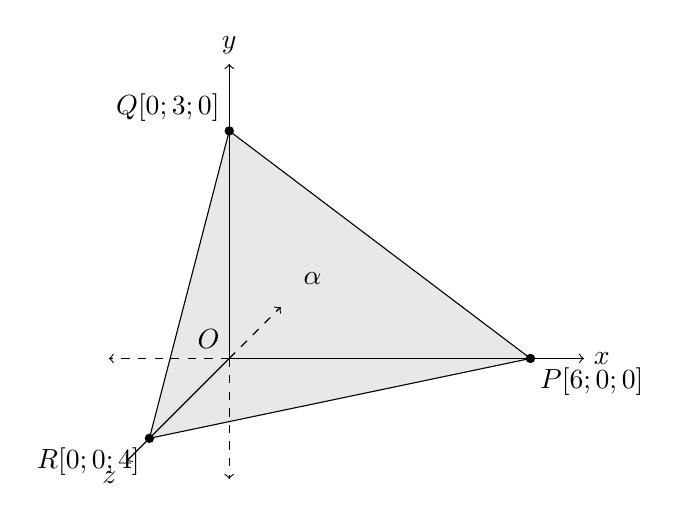
\begin{tikzpicture}[scale=0.85]

        % Průsečíky s osami
        \coordinate (P) at (4.5,0,0);
        \coordinate (Q) at (0,3.4,0);
        \coordinate (R) at (0,0,3.1);

        % Část roviny určená průsečíky
        \fill[gray!18] (P) -- (Q) -- (R) -- cycle;
        \draw[thin] (P) -- (Q) -- (R) -- cycle;

        % Osy - kladná část
        \draw[->] (0,0,0) -- (5.3,0,0) node[right] {$x$};
        \draw[->] (0,0,0) -- (0,4.4,0) node[above] {$y$};
        \draw[->] (0,0,0) -- (0,0,4.0) node[below left] {$z$};

        % Osy - záporná část
        \draw[->, dashed] (0,0,0) -- (-1.8,0,0);
        \draw[->, dashed] (0,0,0) -- (0,-1.8,0);
        \draw[->, dashed] (0,0,0) -- (0,0,-2.0);

        \node[above left] at (0,0,0) {$O$};

        % Body
        \fill (P) circle (2pt) node[below right] {$P[6;0;0]$};
        \fill (Q) circle (2pt) node[above left] {$Q[0;3;0]$};
        \fill (R) circle (2pt) node[below left] {$R[0;0;4]$};

        \node at (1.9,1.85,1.7) {$\alpha$};

    \end{tikzpicture}
    \caption{Rovina určená svými průsečíky se souřadnicovými osami.}
    \label{fig:Plane_intercept_form}
\end{figure}

Úsekový tvar nelze použít v každé situaci. Jestliže je některý
z koeficientů $a$, $b$, $c$ nulový, je rovina rovnoběžná s příslušnou
osou a nemá s ní jediný průsečík. Jestliže rovina prochází počátkem,
je některý z úseků nulový a ve jmenovateli úsekového tvaru by vznikla
nula.

\subsubsection{Shrnutí}
\label{subsubsec:General_plane_summary}

Obecná rovnice roviny má tvar
\[
    ax+by+cz+d=0,
\]
kde alespoň jeden z koeficientů $a$, $b$, $c$ je nenulový.

Z této rovnice můžeme vyčíst normálový vektor
\[
    \vec{n}=(a;b;c).
\]

Bod $P[x_P;y_P;z_P]$ leží v rovině právě tehdy, když po dosazení jeho
souřadnic platí
\[
    ax_P+by_P+cz_P+d=0.
\]

Obecnou rovnici můžeme sestavit zejména tehdy, když známe:

\begin{itemize}
    \item bod roviny a její normálový vektor;
    \item tři nekolineární body roviny;
    \item parametrické vyjádření roviny;
    \item rovinu, se kterou má být hledaná rovina rovnoběžná, a jeden bod;
    \item přímku, ke které má být hledaná rovina kolmá, a jeden bod.
\end{itemize}

Obecná rovnice je vhodná pro ověřování příslušnosti bodů a pro práci
s normálovým směrem roviny. V následujících částech ji využijeme při
zkoumání vzájemné polohy rovin a při určování vztahů mezi přímkami
a rovinami.
